%% Phase 4 research paper -- Springer Nature LaTeX template v3.1 (December 2024), class sn-jnl.
%% Every result is written as \V{key}; the value comes from a committed analysis file through
%% scripts/paper/build_numbers.py, which writes paper/generated/numbers.tex and docs/paper/NUMBERS_MAP.csv.
%% Rebuild: python scripts/paper/build_numbers.py && latexmk -pdf PHASE4_RESEARCH_PAPER.tex (in paper/)
\input{glyphtounicode}\pdfgentounicode=1
\documentclass[pdflatex,iicol,sn-mathphys-num]{sn-jnl}

\usepackage{graphicx}%
\usepackage{multirow}%
\usepackage{amsmath,amssymb,amsfonts}%
\usepackage{amsthm}%
\usepackage{mathrsfs}%
\usepackage[title]{appendix}%
\usepackage{xcolor}%
\usepackage{textcomp}%
\usepackage{manyfoot}%
\usepackage{booktabs}%
\usepackage{algorithm}%
\usepackage{algorithmicx}%
\usepackage{algpseudocode}%
\usepackage{listings}%
\usepackage{tabularx}%
\usepackage{array}%
\newcolumntype{Y}{>{\raggedright\arraybackslash}X}

% generated by scripts/paper/build_numbers.py -- do not edit; every value is in docs/paper/NUMBERS_MAP.csv
\makeatletter
\expandafter\def\csname V@abl:A1|S1-DEB|S1:ci95\endcsname{[\textminus{}0.074, 0.105]}
\expandafter\def\csname V@abl:A1|S1-DEB|S1:delta\endcsname{+0.016}
\expandafter\def\csname V@abl:A1|S1-DEB|S1:p\endcsname{0.731}
\expandafter\def\csname V@abl:A2|S1-DEB|S1:ci95\endcsname{[\textminus{}0.039, 0.141]}
\expandafter\def\csname V@abl:A2|S1-DEB|S1:delta\endcsname{+0.051}
\expandafter\def\csname V@abl:A2|S1-DEB|S1:p\endcsname{0.266}
\expandafter\def\csname V@abl:DEB|S1|impl-DEB|S1:ci95\endcsname{[\textminus{}0.214, 0.045]}
\expandafter\def\csname V@abl:DEB|S1|impl-DEB|S1:delta\endcsname{\textminus{}0.086}
\expandafter\def\csname V@abl:DEB|S1|impl-DEB|S1:p\endcsname{0.193}
\expandafter\def\csname V@abl:DEB|S1|noF-DEB|S1:ci95\endcsname{[\textminus{}0.282, 0.034]}
\expandafter\def\csname V@abl:DEB|S1|noF-DEB|S1:delta\endcsname{\textminus{}0.122}
\expandafter\def\csname V@abl:DEB|S1|noF-DEB|S1:delta@abs\endcsname{0.122}
\expandafter\def\csname V@abl:DEB|S1|noF-DEB|S1:p\endcsname{0.136}
\expandafter\def\csname V@abl:J1|S1|impl-J1|S1:ci95\endcsname{[\textminus{}0.053, 0.122]}
\expandafter\def\csname V@abl:J1|S1|impl-J1|S1:delta\endcsname{+0.036}
\expandafter\def\csname V@abl:J1|S1|impl-J1|S1:p\endcsname{0.406}
\expandafter\def\csname V@abl:J1|S1|noF-J1|S1:ci95\endcsname{[\textminus{}0.314, \textminus{}0.006]}
\expandafter\def\csname V@abl:J1|S1|noF-J1|S1:delta\endcsname{\textminus{}0.163}
\expandafter\def\csname V@abl:J1|S1|noF-J1|S1:p\endcsname{0.042}
\expandafter\def\csname V@abl:J1|S2|specprime-J1|S2:ci95\endcsname{[\textminus{}0.040, 0.132]}
\expandafter\def\csname V@abl:J1|S2|specprime-J1|S2:delta\endcsname{+0.042}
\expandafter\def\csname V@abl:J1|S2|specprime-J1|S2:p\endcsname{0.330}
\expandafter\def\csname V@abl:SC|S1|noF-SC|S1:ci95\endcsname{[\textminus{}0.490, \textminus{}0.083]}
\expandafter\def\csname V@abl:SC|S1|noF-SC|S1:delta\endcsname{\textminus{}0.282}
\expandafter\def\csname V@abl:SC|S1|noF-SC|S1:delta@abs\endcsname{0.282}
\expandafter\def\csname V@abl:SC|S1|noF-SC|S1:p\endcsname{0.003}
\expandafter\def\csname V@aud2:consensus_vs_execution:agreement@pct1\endcsname{97.2\%}
\expandafter\def\csname V@aud2:consensus_vs_execution:kappa_pf_tf\endcsname{0.934}
\expandafter\def\csname V@aud2:llm_rater_secondary_D84:consensus_vs_C:kappa\endcsname{0.903}
\expandafter\def\csname V@aud2:raters:kappa\endcsname{0.936}
\expandafter\def\csname V@aud2:raters:kappa_ci95_bug_bootstrap\endcsname{[0.638, 1.000]}
\expandafter\def\csname V@aud:dev_split_labels:TF\endcsname{89}
\expandafter\def\csname V@aud:labels:PF\endcsname{21}
\expandafter\def\csname V@aud:labels:TF\endcsname{50}
\expandafter\def\csname V@aud:n_items\endcsname{71}
\expandafter\def\csname V@cas1:escalation:share_escalated@pct0\endcsname{61\%}
\expandafter\def\csname V@cas1:summary:CAS|S1:f1\endcsname{0.741}
\expandafter\def\csname V@cas1:summary:CAS|S1:mcc\endcsname{0.595}
\expandafter\def\csname V@cas1:summary:CAS|S1:pf_lost@1\endcsname{10.3}
\expandafter\def\csname V@cas1:summary:DEB|S1|SON:f1\endcsname{0.823}
\expandafter\def\csname V@cas2:escalation:escalated@0\endcsname{134}
\expandafter\def\csname V@cas2:escalation:frontier_calls_all_per_replicate@0\endcsname{1,350}
\expandafter\def\csname V@cas2:escalation:frontier_calls_cascade_per_replicate@0\endcsname{670}
\expandafter\def\csname V@cas2:escalation:share_escalated@pct0\endcsname{50\%}
\expandafter\def\csname V@cas2:escalation:share_escalated@pct1\endcsname{49.6\%}
\expandafter\def\csname V@cas2:escalation:tier1_discard@0\endcsname{35}
\expandafter\def\csname V@cas2:escalation:tier1_keep@0\endcsname{101}
\expandafter\def\csname V@cas2:hypotheses:H12-1:ci95\endcsname{[0.202, 0.460]}
\expandafter\def\csname V@cas2:hypotheses:H12-1:delta\endcsname{+0.311}
\expandafter\def\csname V@cas2:hypotheses:H12-1:p_holm\endcsname{\textless{}0.001}
\expandafter\def\csname V@cas2:hypotheses:H12-2:ci90\endcsname{[\textminus{}0.075, \textminus{}0.022]}
\expandafter\def\csname V@cas2:hypotheses:H12-2:ci95\endcsname{[\textminus{}0.081, \textminus{}0.018]}
\expandafter\def\csname V@cas2:hypotheses:H12-2:delta\endcsname{\textminus{}0.046}
\expandafter\def\csname V@cas2:hypotheses:H12-2:p_holm\endcsname{0.397}
\expandafter\def\csname V@cas2:n_bugs\endcsname{64}
\expandafter\def\csname V@cas2:n_instances\endcsname{270}
\expandafter\def\csname V@cas2:summary:CASJ1|S1:f1\endcsname{0.833}
\expandafter\def\csname V@cas2:summary:CASJ1|S1:mcc\endcsname{0.606}
\expandafter\def\csname V@cas2:summary:CASJ1|S1:pf_lost@0\endcsname{24}
\expandafter\def\csname V@cas2:summary:CASJ1|S1:precision\endcsname{0.823}
\expandafter\def\csname V@cas2:summary:CASJ1|S1:recall\endcsname{0.844}
\expandafter\def\csname V@cas2:summary:CAS|S1:f1\endcsname{0.863}
\expandafter\def\csname V@cas2:summary:CAS|S1:mcc\endcsname{0.666}
\expandafter\def\csname V@cas2:summary:CAS|S1:pf_lost@0\endcsname{15}
\expandafter\def\csname V@cas2:summary:CAS|S1:precision\endcsname{0.827}
\expandafter\def\csname V@cas2:summary:CAS|S1:recall\endcsname{0.903}
\expandafter\def\csname V@cas2:summary:DEB|S1:f1\endcsname{0.700}
\expandafter\def\csname V@cas2:summary:DEB|S1:mcc\endcsname{0.392}
\expandafter\def\csname V@cas2:summary:DEB|S1:pf_lost@0\endcsname{56}
\expandafter\def\csname V@cas2:summary:DEB|S1:precision\endcsname{0.778}
\expandafter\def\csname V@cas2:summary:DEB|S1:recall\endcsname{0.636}
\expandafter\def\csname V@cas2:summary:DEB|S1|SON:f1\endcsname{0.910}
\expandafter\def\csname V@cas2:summary:DEB|S1|SON:mcc\endcsname{0.788}
\expandafter\def\csname V@cas2:summary:DEB|S1|SON:pf_lost@0\endcsname{13}
\expandafter\def\csname V@cas2:summary:DEB|S1|SON:precision\endcsname{0.904}
\expandafter\def\csname V@cas2:summary:DEB|S1|SON:recall\endcsname{0.916}
\expandafter\def\csname V@cas2:summary:J1|S1|SON:f1\endcsname{0.845}
\expandafter\def\csname V@cas2:summary:J1|S1|SON:mcc\endcsname{0.687}
\expandafter\def\csname V@cas2:summary:J1|S1|SON:pf_lost@0\endcsname{34}
\expandafter\def\csname V@cas2:summary:J1|S1|SON:precision\endcsname{0.923}
\expandafter\def\csname V@cas2:summary:J1|S1|SON:recall\endcsname{0.779}
\expandafter\def\csname V@cas2:summary:KUU|S1:f1\endcsname{0.771}
\expandafter\def\csname V@cas2:summary:KUU|S1:mcc\endcsname{0.356}
\expandafter\def\csname V@cas2:summary:KUU|S1:pf_lost@0\endcsname{4}
\expandafter\def\csname V@cas2:summary:KUU|S1:precision\endcsname{0.638}
\expandafter\def\csname V@cas2:summary:KUU|S1:recall\endcsname{0.974}
\expandafter\def\csname V@cfgt0:temperature@1\endcsname{0.0}
\expandafter\def\csname V@cfgth:max_tokens@int\endcsname{8,192}
\expandafter\def\csname V@cfgth:spec_patch:num_ctx@int\endcsname{16,384}
\expandafter\def\csname V@cit:candor hi\endcsname{0.930}
\expandafter\def\csname V@cit:candor lo\endcsname{0.894}
\expandafter\def\csname V@cit:chatassert\endcsname{15}
\expandafter\def\csname V@cit:javaoracle precision\endcsname{0.889}
\expandafter\def\csname V@cit:javaoracle tp after\endcsname{5.33}
\expandafter\def\csname V@cit:javaoracle tp before\endcsname{14.33}
\expandafter\def\csname V@cit:jstestcraft audit n\endcsname{296}
\expandafter\def\csname V@cit:jstestcraft branch\endcsname{47.3}
\expandafter\def\csname V@cit:jstestcraft pass\endcsname{60.9}
\expandafter\def\csname V@cit:jstestcraft recall\endcsname{68.75}
\expandafter\def\csname V@cit:jstestcraft repos\endcsname{20}
\expandafter\def\csname V@cit:maco branch\endcsname{79.2}
\expandafter\def\csname V@cit:maco line\endcsname{84.4}
\expandafter\def\csname V@cit:maco methods\endcsname{41}
\expandafter\def\csname V@cit:maddila solve\endcsname{42.3}
\expandafter\def\csname V@cit:mitgen base\endcsname{0.31}
\expandafter\def\csname V@cit:mitgen ours\endcsname{0.66}
\expandafter\def\csname V@cit:target em\endcsname{66.1}
\expandafter\def\csname V@cit:testart pass\endcsname{78.55}
\expandafter\def\csname V@cit:valtest\endcsname{29}
\expandafter\def\csname V@cit:walczak docstring\endcsname{19.67}
\expandafter\def\csname V@cit:walczak methods\endcsname{12}
\expandafter\def\csname V@cit:zhao hi\endcsname{4.54}
\expandafter\def\csname V@cit:zhao lo\endcsname{2.09}
\expandafter\def\csname V@conf:f1:H1:ci90\endcsname{[0.026, 0.345]}
\expandafter\def\csname V@conf:f1:H1:ci95\endcsname{[\textminus{}0.006, 0.370]}
\expandafter\def\csname V@conf:f1:H1:delta\endcsname{+0.195}
\expandafter\def\csname V@conf:f1:H1:p\endcsname{0.058}
\expandafter\def\csname V@conf:f1:H1:p_holm\endcsname{0.233}
\expandafter\def\csname V@conf:f1:H2a:ci95\endcsname{[\textminus{}0.091, \textminus{}0.006]}
\expandafter\def\csname V@conf:f1:H2a:delta\endcsname{\textminus{}0.050}
\expandafter\def\csname V@conf:f1:H2a:p\endcsname{0.023}
\expandafter\def\csname V@conf:f1:H2a:p_holm\endcsname{0.116}
\expandafter\def\csname V@conf:f1:H2b:ci95\endcsname{[\textminus{}0.024, 0.064]}
\expandafter\def\csname V@conf:f1:H2b:delta\endcsname{+0.019}
\expandafter\def\csname V@conf:f1:H2b:p\endcsname{0.399}
\expandafter\def\csname V@conf:f1:H2b:p_holm\endcsname{0.798}
\expandafter\def\csname V@conf:f1:H3a:ci95\endcsname{[\textminus{}0.031, 0.201]}
\expandafter\def\csname V@conf:f1:H3a:delta\endcsname{+0.074}
\expandafter\def\csname V@conf:f1:H3a:p\endcsname{0.177}
\expandafter\def\csname V@conf:f1:H3a:p_holm\endcsname{0.532}
\expandafter\def\csname V@conf:f1:H3b:ci95\endcsname{[\textminus{}0.104, 0.055]}
\expandafter\def\csname V@conf:f1:H3b:delta\endcsname{\textminus{}0.024}
\expandafter\def\csname V@conf:f1:H3b:p\endcsname{0.524}
\expandafter\def\csname V@conf:f1:H3b:p_holm\endcsname{0.798}
\expandafter\def\csname V@conf:secondary:H1~precision:delta\endcsname{+0.167}
\expandafter\def\csname V@conf:secondary:H1~precision:p_holm\endcsname{0.715}
\expandafter\def\csname V@conf:secondary:H1~recall:delta\endcsname{+0.222}
\expandafter\def\csname V@conf:secondary:H1~recall:p_holm\endcsname{0.437}
\expandafter\def\csname V@conf:secondary:H2a~precision:delta\endcsname{\textminus{}0.041}
\expandafter\def\csname V@conf:secondary:H2a~precision:p_holm\endcsname{0.638}
\expandafter\def\csname V@conf:secondary:H2a~recall:delta\endcsname{\textminus{}0.061}
\expandafter\def\csname V@conf:secondary:H2a~recall:p_holm\endcsname{0.220}
\expandafter\def\csname V@conf:secondary:H2b~precision:ci90\endcsname{[\textminus{}0.041, 0.040]}
\expandafter\def\csname V@conf:secondary:H2b~precision:delta\endcsname{\textminus{}0.002}
\expandafter\def\csname V@conf:secondary:H2b~precision:p_holm\endcsname{1.000}
\expandafter\def\csname V@conf:secondary:H2b~recall:delta\endcsname{+0.037}
\expandafter\def\csname V@conf:secondary:H2b~recall:p_holm\endcsname{0.715}
\expandafter\def\csname V@conf:secondary:H3a~precision:delta\endcsname{+0.043}
\expandafter\def\csname V@conf:secondary:H3a~precision:p_holm\endcsname{1.000}
\expandafter\def\csname V@conf:secondary:H3a~recall:delta\endcsname{+0.100}
\expandafter\def\csname V@conf:secondary:H3a~recall:p_holm\endcsname{0.715}
\expandafter\def\csname V@conf:secondary:H3b~precision:delta\endcsname{+0.030}
\expandafter\def\csname V@conf:secondary:H3b~precision:p_holm\endcsname{1.000}
\expandafter\def\csname V@conf:secondary:H3b~recall:delta\endcsname{\textminus{}0.072}
\expandafter\def\csname V@conf:secondary:H3b~recall:p_holm\endcsname{0.715}
\expandafter\def\csname V@cost:arms:DEB:calls_per_instance@0\endcsname{5}
\expandafter\def\csname V@cost:arms:DEB:input_tokens_per_instance@0\endcsname{8,459}
\expandafter\def\csname V@cost:arms:DEB:output_tokens_per_instance@0\endcsname{729}
\expandafter\def\csname V@cost:arms:DEB:replicates\endcsname{3}
\expandafter\def\csname V@cost:arms:DEB:wall_s_median@1\endcsname{12.9}
\expandafter\def\csname V@cost:arms:DEB:wall_s_median@2\endcsname{12.94}
\expandafter\def\csname V@cost:arms:DEB:wall_s_p90@2\endcsname{15.77}
\expandafter\def\csname V@cost:arms:J1:calls_per_instance@0\endcsname{1}
\expandafter\def\csname V@cost:arms:J1:input_tokens_per_instance@0\endcsname{1,811}
\expandafter\def\csname V@cost:arms:J1:output_tokens_per_instance@0\endcsname{103}
\expandafter\def\csname V@cost:arms:J1:wall_s_median@1\endcsname{1.7}
\expandafter\def\csname V@cost:arms:J1:wall_s_median@2\endcsname{1.71}
\expandafter\def\csname V@cost:arms:J1:wall_s_p90@2\endcsname{2.19}
\expandafter\def\csname V@cost:arms:SC-T:calls_per_instance@0\endcsname{5}
\expandafter\def\csname V@cost:arms:SC-T:input_tokens_per_instance@0\endcsname{9,054}
\expandafter\def\csname V@cost:arms:SC-T:output_tokens_per_instance@0\endcsname{496}
\expandafter\def\csname V@cost:arms:SC-T:wall_s_median@2\endcsname{7.71}
\expandafter\def\csname V@cost:arms:SC-T:wall_s_p90@2\endcsname{9.51}
\expandafter\def\csname V@cost:arms:SC:calls_per_instance@0\endcsname{5}
\expandafter\def\csname V@cost:arms:SC:input_tokens_per_instance@0\endcsname{9,054}
\expandafter\def\csname V@cost:arms:SC:output_tokens_per_instance@0\endcsname{497}
\expandafter\def\csname V@cost:arms:SC:wall_s_median@2\endcsname{7.59}
\expandafter\def\csname V@cost:arms:SC:wall_s_p90@2\endcsname{9.67}
\expandafter\def\csname V@cost:deb_over_j1:median_wall@1\endcsname{7.6}
\expandafter\def\csname V@cost:deb_over_j1:tokens@1\endcsname{4.8}
\expandafter\def\csname V@cost:scored_instances\endcsname{177}
\expandafter\def\csname V@d1:A1|S1:f1\endcsname{0.526}
\expandafter\def\csname V@d1:A1|S1:mcc\endcsname{0.249}
\expandafter\def\csname V@d1:A2|S1:f1\endcsname{0.561}
\expandafter\def\csname V@d1:A2|S1:mcc\endcsname{0.293}
\expandafter\def\csname V@d1:DA:f1\endcsname{0}
\expandafter\def\csname V@d1:DA:mcc\endcsname{0}
\expandafter\def\csname V@d1:DA:pf_lost\endcsname{60}
\expandafter\def\csname V@d1:DA:pf_lost@0\endcsname{60}
\expandafter\def\csname V@d1:DA:recall\endcsname{0}
\expandafter\def\csname V@d1:DEB|S0:f1\endcsname{0.550}
\expandafter\def\csname V@d1:DEB|S0:mcc\endcsname{0.311}
\expandafter\def\csname V@d1:DEB|S1:TN@1\endcsname{89.3}
\expandafter\def\csname V@d1:DEB|S1:calls_per_instance\endcsname{5}
\expandafter\def\csname V@d1:DEB|S1:consumed_tokens_per_instance@0\endcsname{9,188}
\expandafter\def\csname V@d1:DEB|S1:delta_f1_vs_J1_per_1k_tokens@4\endcsname{0.0069}
\expandafter\def\csname V@d1:DEB|S1:f1\endcsname{0.511}
\expandafter\def\csname V@d1:DEB|S1:f1_ci95\endcsname{[0.378, 0.613]}
\expandafter\def\csname V@d1:DEB|S1:invalid_rate@pct\endcsname{0.0\%}
\expandafter\def\csname V@d1:DEB|S1:latency_s_per_instance@1\endcsname{13.3}
\expandafter\def\csname V@d1:DEB|S1:mcc\endcsname{0.267}
\expandafter\def\csname V@d1:DEB|S1:mcc_ci95\endcsname{[0.126, 0.405]}
\expandafter\def\csname V@d1:DEB|S1:no_evidence_rate@pct\endcsname{0.0\%}
\expandafter\def\csname V@d1:DEB|S1:pf_lost@0\endcsname{30}
\expandafter\def\csname V@d1:DEB|S1:pf_lost@1\endcsname{30.0}
\expandafter\def\csname V@d1:DEB|S1:position_bias_rate@pct\endcsname{52.6\%}
\expandafter\def\csname V@d1:DEB|S1:precision\endcsname{0.523}
\expandafter\def\csname V@d1:DEB|S1:precision_prev_adj\endcsname{0.315}
\expandafter\def\csname V@d1:DEB|S1:recall\endcsname{0.500}
\expandafter\def\csname V@d1:DEB|S1|impl:f1\endcsname{0.425}
\expandafter\def\csname V@d1:DEB|S1|impl:mcc\endcsname{0.164}
\expandafter\def\csname V@d1:DEB|S1|noF:f1\endcsname{0.389}
\expandafter\def\csname V@d1:DEB|S1|noF:mcc\endcsname{0.127}
\expandafter\def\csname V@d1:DEB|S2:f1\endcsname{0.493}
\expandafter\def\csname V@d1:DEB|S2:mcc\endcsname{0.228}
\expandafter\def\csname V@d1:J1|S0:f1\endcsname{0.494}
\expandafter\def\csname V@d1:J1|S0:mcc\endcsname{0.220}
\expandafter\def\csname V@d1:J1|S1:calls_per_instance\endcsname{1}
\expandafter\def\csname V@d1:J1|S1:consumed_tokens_per_instance@0\endcsname{1,913}
\expandafter\def\csname V@d1:J1|S1:f1\endcsname{0.460}
\expandafter\def\csname V@d1:J1|S1:f1_ci95\endcsname{[0.329, 0.556]}
\expandafter\def\csname V@d1:J1|S1:invalid_rate@pct\endcsname{1.7\%}
\expandafter\def\csname V@d1:J1|S1:latency_s_per_instance@1\endcsname{1.9}
\expandafter\def\csname V@d1:J1|S1:mcc\endcsname{0.174}
\expandafter\def\csname V@d1:J1|S1:mcc_ci95\endcsname{[0.032, 0.300]}
\expandafter\def\csname V@d1:J1|S1:pf_lost@1\endcsname{31.7}
\expandafter\def\csname V@d1:J1|S1:precision\endcsname{0.450}
\expandafter\def\csname V@d1:J1|S1:precision_prev_adj\endcsname{0.250}
\expandafter\def\csname V@d1:J1|S1:recall\endcsname{0.472}
\expandafter\def\csname V@d1:J1|S1|impl:f1\endcsname{0.488}
\expandafter\def\csname V@d1:J1|S1|impl:mcc\endcsname{0.222}
\expandafter\def\csname V@d1:J1|S1|noF:f1\endcsname{0.297}
\expandafter\def\csname V@d1:J1|S1|noF:mcc\endcsname{0.031}
\expandafter\def\csname V@d1:J1|S2:f1\endcsname{0.477}
\expandafter\def\csname V@d1:J1|S2:mcc\endcsname{0.202}
\expandafter\def\csname V@d1:J1|S2|specprime:f1\endcsname{0.518}
\expandafter\def\csname V@d1:J1|S2|specprime:mcc\endcsname{0.231}
\expandafter\def\csname V@d1:KA:f1\endcsname{0.506}
\expandafter\def\csname V@d1:KA:f1_ci95\endcsname{[0.355, 0.633]}
\expandafter\def\csname V@d1:KA:mcc\endcsname{0}
\expandafter\def\csname V@d1:KA:pf_lost\endcsname{0}
\expandafter\def\csname V@d1:KA:precision\endcsname{0.339}
\expandafter\def\csname V@d1:KA:precision_prev_adj\endcsname{0.172}
\expandafter\def\csname V@d1:KA:recall\endcsname{1}
\expandafter\def\csname V@d1:R0:f1\endcsname{0.266}
\expandafter\def\csname V@d1:R0:f1_ci95\endcsname{[0.110, 0.429]}
\expandafter\def\csname V@d1:R0:mcc\endcsname{\textminus{}0.077}
\expandafter\def\csname V@d1:R0:mcc_ci95\endcsname{[\textminus{}0.284, 0.158]}
\expandafter\def\csname V@d1:R0:pf_lost\endcsname{45}
\expandafter\def\csname V@d1:R0:pf_lost@0\endcsname{45}
\expandafter\def\csname V@d1:R0:precision\endcsname{0.283}
\expandafter\def\csname V@d1:R0:precision_prev_adj\endcsname{0.139}
\expandafter\def\csname V@d1:R0:recall\endcsname{0.250}
\expandafter\def\csname V@d1:SC-T|S1:calls_per_instance\endcsname{5}
\expandafter\def\csname V@d1:SC-T|S1:consumed_tokens_per_instance@0\endcsname{9,550}
\expandafter\def\csname V@d1:SC-T|S1:delta_f1_vs_J1_per_1k_tokens@4\endcsname{0.0005}
\expandafter\def\csname V@d1:SC-T|S1:f1\endcsname{0.464}
\expandafter\def\csname V@d1:SC-T|S1:f1_ci95\endcsname{[0.289, 0.593]}
\expandafter\def\csname V@d1:SC-T|S1:invalid_rate@pct\endcsname{0.0\%}
\expandafter\def\csname V@d1:SC-T|S1:latency_s_per_instance@1\endcsname{8.1}
\expandafter\def\csname V@d1:SC-T|S1:mcc\endcsname{0.238}
\expandafter\def\csname V@d1:SC-T|S1:mcc_ci95\endcsname{[0.040, 0.408]}
\expandafter\def\csname V@d1:SC-T|S1:pf_lost@1\endcsname{35.0}
\expandafter\def\csname V@d1:SC-T|S1:precision\endcsname{0.524}
\expandafter\def\csname V@d1:SC-T|S1:precision_prev_adj\endcsname{0.311}
\expandafter\def\csname V@d1:SC-T|S1:recall\endcsname{0.417}
\expandafter\def\csname V@d1:SC|S0:f1\endcsname{0.502}
\expandafter\def\csname V@d1:SC|S0:mcc\endcsname{0.290}
\expandafter\def\csname V@d1:SC|S1:calls_per_instance\endcsname{5}
\expandafter\def\csname V@d1:SC|S1:consumed_tokens_per_instance@0\endcsname{9,551}
\expandafter\def\csname V@d1:SC|S1:delta_f1_vs_J1_per_1k_tokens@4\endcsname{\textminus{}0.0031}
\expandafter\def\csname V@d1:SC|S1:f1\endcsname{0.436}
\expandafter\def\csname V@d1:SC|S1:f1_ci95\endcsname{[0.263, 0.573]}
\expandafter\def\csname V@d1:SC|S1:invalid_rate@pct\endcsname{0.0\%}
\expandafter\def\csname V@d1:SC|S1:latency_s_per_instance@1\endcsname{8.1}
\expandafter\def\csname V@d1:SC|S1:mcc\endcsname{0.187}
\expandafter\def\csname V@d1:SC|S1:mcc_ci95\endcsname{[\textminus{}0.012, 0.366]}
\expandafter\def\csname V@d1:SC|S1:pf_lost@0\endcsname{36}
\expandafter\def\csname V@d1:SC|S1:pf_lost@1\endcsname{36.0}
\expandafter\def\csname V@d1:SC|S1:precision\endcsname{0.480}
\expandafter\def\csname V@d1:SC|S1:precision_prev_adj\endcsname{0.272}
\expandafter\def\csname V@d1:SC|S1:recall\endcsname{0.400}
\expandafter\def\csname V@d1:SC|S1|noF:f1\endcsname{0.154}
\expandafter\def\csname V@d1:SC|S1|noF:mcc\endcsname{\textminus{}0.004}
\expandafter\def\csname V@d1:SC|S2:f1\endcsname{0.493}
\expandafter\def\csname V@d1:SC|S2:mcc\endcsname{0.232}
\expandafter\def\csname V@d1m2:DEB|S1:f1\endcsname{0.727}
\expandafter\def\csname V@d1m2:DEB|S1:mcc\endcsname{0.571}
\expandafter\def\csname V@d1m2:J1|S1:f1\endcsname{0.599}
\expandafter\def\csname V@d1m2:J1|S1:mcc\endcsname{0.358}
\expandafter\def\csname V@d1m2:SC|S1:f1\endcsname{0.599}
\expandafter\def\csname V@d1m2:SC|S1:mcc\endcsname{0.358}
\expandafter\def\csname V@d2:DEB|S1:f1\endcsname{0.700}
\expandafter\def\csname V@d2:DEB|S1:mcc\endcsname{0.392}
\expandafter\def\csname V@d2:DEB|S1:n_instances\endcsname{270}
\expandafter\def\csname V@d2:DEB|S2:f1\endcsname{0.758}
\expandafter\def\csname V@d2:DEB|S2:mcc\endcsname{0.463}
\expandafter\def\csname V@d2:J1|S1:f1\endcsname{0.647}
\expandafter\def\csname V@d2:J1|S1:mcc\endcsname{0.301}
\expandafter\def\csname V@d2:KA:f1\endcsname{0.726}
\expandafter\def\csname V@d2:KA:mcc\endcsname{0}
\expandafter\def\csname V@d2:R0:f1\endcsname{0.528}
\expandafter\def\csname V@d2:R0:mcc\endcsname{0.082}
\expandafter\def\csname V@d2:SC|S1:f1\endcsname{0.708}
\expandafter\def\csname V@d2:SC|S1:mcc\endcsname{0.383}
\expandafter\def\csname V@d2m2:DEB|S1:f1\endcsname{0.855}
\expandafter\def\csname V@d2m2:DEB|S1:mcc\endcsname{0.644}
\expandafter\def\csname V@d2m2:J1|S1:f1\endcsname{0.787}
\expandafter\def\csname V@d2m2:J1|S1:mcc\endcsname{0.420}
\expandafter\def\csname V@d2m2:SC|S1:f1\endcsname{0.784}
\expandafter\def\csname V@d2m2:SC|S1:mcc\endcsname{0.410}
\expandafter\def\csname V@d2rep:before_cap:d2_units_total\endcsname{284}
\expandafter\def\csname V@d2rep:before_cap:labelled_instances:AMB\endcsname{65}
\expandafter\def\csname V@d2rep:before_cap:labelled_instances:PF\endcsname{468}
\expandafter\def\csname V@d2rep:before_cap:labelled_instances:TF\endcsname{349}
\expandafter\def\csname V@d2rep:judged_sample:cap\endcsname{300}
\expandafter\def\csname V@der:d1 DEB S1-S0 f1\endcsname{\textminus{}0.040}
\expandafter\def\csname V@der:d1 DEB-J1 f1\endcsname{+0.050}
\expandafter\def\csname V@der:d1 DEB-J1 f1 rel@spct\endcsname{+10.9\%}
\expandafter\def\csname V@der:d1 DEB-KA f1\endcsname{+0.004}
\expandafter\def\csname V@der:d1 DEB-KA f1 rel@spct\endcsname{+0.8\%}
\expandafter\def\csname V@der:d1 DEB-R0 f1\endcsname{+0.245}
\expandafter\def\csname V@der:d1 DEB-R0 f1 rel@spct\endcsname{+92.3\%}
\expandafter\def\csname V@der:d1 DEB-R0 mcc\endcsname{+0.344}
\expandafter\def\csname V@der:d1 DEB-SC f1 rel@spct\endcsname{+17.1\%}
\expandafter\def\csname V@der:d1 J1 S1-S0 f1\endcsname{\textminus{}0.034}
\expandafter\def\csname V@der:d1 SC S1-S0 f1\endcsname{\textminus{}0.066}
\expandafter\def\csname V@der:d1 best S1 LLM - KA f1@abs\endcsname{0.004}
\expandafter\def\csname V@der:d1 best S1 LLM is DEB\endcsname{DEB}
\expandafter\def\csname V@der:d1 test AMB labelled\endcsname{13}
\expandafter\def\csname V@der:d1 test PF labelled\endcsname{60}
\expandafter\def\csname V@der:d1 test TF labelled\endcsname{296}
\expandafter\def\csname V@der:d2 SC-DEB f1\endcsname{+0.008}
\expandafter\def\csname V@der:d2 aborted instances\endcsname{8}
\expandafter\def\csname V@der:d2 aborts mutated line\endcsname{5}
\expandafter\def\csname V@der:dev methods\endcsname{39}
\expandafter\def\csname V@der:gate M1 G_a\endcsname{pass}
\expandafter\def\csname V@der:gate M1 G_b\endcsname{pass}
\expandafter\def\csname V@der:gate M1 G_c\endcsname{pass}
\expandafter\def\csname V@der:gate M1 G_d\endcsname{fail}
\expandafter\def\csname V@der:gate M2 G_a\endcsname{pass}
\expandafter\def\csname V@der:gate M2 G_b\endcsname{pass}
\expandafter\def\csname V@der:gate M2 G_c\endcsname{pass}
\expandafter\def\csname V@der:gate M2 G_d\endcsname{fail}
\expandafter\def\csname V@der:gate M3 G_a\endcsname{pass}
\expandafter\def\csname V@der:gate M3 G_b\endcsname{pass}
\expandafter\def\csname V@der:gate M3 G_c\endcsname{pass}
\expandafter\def\csname V@der:gate M3 G_d\endcsname{fail}
\expandafter\def\csname V@der:gate NG G_a\endcsname{pass}
\expandafter\def\csname V@der:gate NG G_b\endcsname{pass}
\expandafter\def\csname V@der:gate NG G_c\endcsname{pass}
\expandafter\def\csname V@der:gate NG G_d\endcsname{fail}
\expandafter\def\csname V@der:holm all match\endcsname{all}
\expandafter\def\csname V@der:holm families\endcsname{10}
\expandafter\def\csname V@der:inv keep max dBA@3\endcsname{0.008}
\expandafter\def\csname V@der:local judges failing G-d@int\endcsname{4}
\expandafter\def\csname V@der:local judges gated\endcsname{4}
\expandafter\def\csname V@der:n test projects\endcsname{14}
\expandafter\def\csname V@der:test methods\endcsname{195}
\expandafter\def\csname V@der:tf176 n\endcsname{176}
\expandafter\def\csname V@devgate:G_d_detail:J1_f1\endcsname{0.350}
\expandafter\def\csname V@devgate:G_d_detail:J1_mcc\endcsname{\textminus{}0.032}
\expandafter\def\csname V@devgate:G_d_detail:R0_f1\endcsname{0.642}
\expandafter\def\csname V@devgate:G_d_detail:R0_mcc\endcsname{0.363}
\expandafter\def\csname V@devgate:G_d_detail:delta_ci95_bug_bootstrap\endcsname{[\textminus{}0.507, 0.596]}
\expandafter\def\csname V@devgate:n_bugs\endcsname{12}
\expandafter\def\csname V@devgate:n_instances\endcsname{55}
\expandafter\def\csname V@ds1:exclusions:MISGUIDED\endcsname{102}
\expandafter\def\csname V@ds1:exclusions:NC\endcsname{518}
\expandafter\def\csname V@ds1:exclusions:PASS\endcsname{2,284}
\expandafter\def\csname V@ds1:exclusions:TIMEOUT\endcsname{6}
\expandafter\def\csname V@ds1:executed_methods\endcsname{2,909}
\expandafter\def\csname V@e6a:35b_minus:DEB 35B-M1:f1:ci95\endcsname{[0.018, 0.247]}
\expandafter\def\csname V@e6a:35b_minus:DEB 35B-M1:f1:delta\endcsname{+0.133}
\expandafter\def\csname V@e6a:n_instances\endcsname{177}
\expandafter\def\csname V@e6a:summary:35B:DEB:f1\endcsname{0.644}
\expandafter\def\csname V@e6a:summary:35B:DEB:mcc\endcsname{0.426}
\expandafter\def\csname V@e6a:summary:35B:J1:f1\endcsname{0.576}
\expandafter\def\csname V@e6a:summary:35B:J1:mcc\endcsname{0.317}
\expandafter\def\csname V@e6a:summary:M1:DEB:f1\endcsname{0.511}
\expandafter\def\csname V@e6b:family_check:e6b_minus:DEB E6B-M1:f1:ci95\endcsname{[\textminus{}0.035, 0.193]}
\expandafter\def\csname V@e6b:family_check:e6b_minus:DEB E6B-M1:f1:delta\endcsname{+0.081}
\expandafter\def\csname V@e6b:family_check:e6b_minus:DEB E6B-M2:f1:ci95\endcsname{[\textminus{}0.223, \textminus{}0.039]}
\expandafter\def\csname V@e6b:family_check:e6b_minus:DEB E6B-M2:f1:delta\endcsname{\textminus{}0.135}
\expandafter\def\csname V@e6b:hypotheses:H6-1:ci95\endcsname{[\textminus{}0.033, 0.080]}
\expandafter\def\csname V@e6b:hypotheses:H6-1:delta\endcsname{+0.022}
\expandafter\def\csname V@e6b:hypotheses:H6-1:p_holm\endcsname{0.419}
\expandafter\def\csname V@e6b:hypotheses:H6-2:ci95\endcsname{[0.226, 0.435]}
\expandafter\def\csname V@e6b:hypotheses:H6-2:mcc\endcsname{0.337}
\expandafter\def\csname V@e6b:hypotheses:H6-2:p_holm\endcsname{\textless{}0.001}
\expandafter\def\csname V@e6b:hypotheses:H6-3:ci95\endcsname{[\textminus{}0.021, 0.035]}
\expandafter\def\csname V@e6b:hypotheses:H6-3:delta\endcsname{+0.004}
\expandafter\def\csname V@e6b:hypotheses:H6-3:tau\endcsname{80}
\expandafter\def\csname V@e6b:n_bugs\endcsname{60}
\expandafter\def\csname V@e6b:n_instances\endcsname{177}
\expandafter\def\csname V@e6b:pf_prevalence:PF\endcsname{60}
\expandafter\def\csname V@e6b:summary:DEB:f1\endcsname{0.592}
\expandafter\def\csname V@e6b:summary:DEB:mcc\endcsname{0.337}
\expandafter\def\csname V@e6b:summary:J1:f1\endcsname{0.555}
\expandafter\def\csname V@e6b:summary:J1:mcc\endcsname{0.234}
\expandafter\def\csname V@e6b:summary:SC:f1\endcsname{0.570}
\expandafter\def\csname V@e6b:summary:SC:mcc\endcsname{0.274}
\expandafter\def\csname V@e7a:tried:0:C1\endcsname{0.378}
\expandafter\def\csname V@e7a:tried:0:C1@2\endcsname{0.38}
\expandafter\def\csname V@e7a:tried:0:C1_ci95\endcsname{[0.270, 0.490]}
\expandafter\def\csname V@e7a:tried:0:C2\endcsname{0.555}
\expandafter\def\csname V@e7a:tried:0:P1\endcsname{0.136}
\expandafter\def\csname V@e7a:tried:1:C1\endcsname{0.166}
\expandafter\def\csname V@e7a:tried:1:C1@2\endcsname{0.17}
\expandafter\def\csname V@e7a:tried:1:C1_ci95\endcsname{[0.099, 0.241]}
\expandafter\def\csname V@e7a:tried:1:C2\endcsname{0.359}
\expandafter\def\csname V@e7a:tried:1:C2_ci95\endcsname{[0.210, 0.519]}
\expandafter\def\csname V@e7a:tried:1:unparseable_classes\endcsname{2}
\expandafter\def\csname V@e8:fresh_j1:M2:f1\endcsname{0.606}
\expandafter\def\csname V@e8:hypotheses:H8-1:ci95\endcsname{[0.024, 0.279]}
\expandafter\def\csname V@e8:hypotheses:H8-1:delta\endcsname{+0.150}
\expandafter\def\csname V@e8:hypotheses:H8-1:p\endcsname{0.021}
\expandafter\def\csname V@e8:hypotheses:H8-1:p_holm\endcsname{0.063}
\expandafter\def\csname V@e8:hypotheses:H8-2:ci95\endcsname{[\textminus{}0.004, 0.289]}
\expandafter\def\csname V@e8:hypotheses:H8-2:delta\endcsname{+0.138}
\expandafter\def\csname V@e8:hypotheses:H8-2:p_holm\endcsname{0.113}
\expandafter\def\csname V@e8:hypotheses:H8-3:ci95\endcsname{[\textminus{}0.055, 0.182]}
\expandafter\def\csname V@e8:hypotheses:H8-3:delta\endcsname{+0.064}
\expandafter\def\csname V@e8:hypotheses:H8-3:p_holm\endcsname{0.285}
\expandafter\def\csname V@e8:summary:DEB|S1:f1\endcsname{0.511}
\expandafter\def\csname V@e8:summary:DEB|S1:pf_lost@0\endcsname{30}
\expandafter\def\csname V@e8:summary:SC3|S1:f1\endcsname{0.463}
\expandafter\def\csname V@e8:summary:SC|S1:f1\endcsname{0.436}
\expandafter\def\csname V@e8:summary:SC|S1:pf_lost@0\endcsname{36}
\expandafter\def\csname V@e8:summary:VOTE3|S1:f1\endcsname{0.614}
\expandafter\def\csname V@e8:summary:VOTE3|S1:mcc\endcsname{0.369}
\expandafter\def\csname V@e8:summary:VOTE3|S1:pf_lost@0\endcsname{6}
\expandafter\def\csname V@e8:summary:VOTE3|S1:precision\endcsname{0.466}
\expandafter\def\csname V@e8:summary:VOTE3|S1:recall\endcsname{0.900}
\expandafter\def\csname V@e8:summary:VOTE3|S1:recall@pct0\endcsname{90\%}
\expandafter\def\csname V@e8:summary:VOTE5|S1:f1\endcsname{0.575}
\expandafter\def\csname V@e8:summary:VOTE5|S1:mcc\endcsname{0.282}
\expandafter\def\csname V@e8:summary:VOTE5|S1:pf_lost@0\endcsname{8}
\expandafter\def\csname V@e9:deb_run_to_run_spread:m1:f1:per_replicate:0\endcsname{0.525}
\expandafter\def\csname V@e9:deb_run_to_run_spread:m1:f1:per_replicate:1\endcsname{0.614}
\expandafter\def\csname V@e9:deb_run_to_run_spread:m1:f1:per_replicate:2\endcsname{0.393}
\expandafter\def\csname V@e9:deb_run_to_run_spread:m1:f1:range\endcsname{0.221}
\expandafter\def\csname V@e9:deb_run_to_run_spread:sonnet:f1:per_replicate:0\endcsname{0.814}
\expandafter\def\csname V@e9:deb_run_to_run_spread:sonnet:f1:per_replicate:1\endcsname{0.838}
\expandafter\def\csname V@e9:deb_run_to_run_spread:sonnet:f1:per_replicate:2\endcsname{0.817}
\expandafter\def\csname V@e9:deb_run_to_run_spread:sonnet:f1:range\endcsname{0.024}
\expandafter\def\csname V@e9:hypotheses:H9-1:ci95\endcsname{[0.003, 0.176]}
\expandafter\def\csname V@e9:hypotheses:H9-1:delta\endcsname{+0.077}
\expandafter\def\csname V@e9:hypotheses:H9-1:p_holm\endcsname{0.040}
\expandafter\def\csname V@e9:hypotheses:H9-2:ci95\endcsname{[0.549, 0.867]}
\expandafter\def\csname V@e9:hypotheses:H9-2:mcc\endcsname{0.734}
\expandafter\def\csname V@e9:hypotheses:H9-2:p_holm\endcsname{\textless{}0.001}
\expandafter\def\csname V@e9:n_instances\endcsname{177}
\expandafter\def\csname V@e9:sonnet_minus_m1:DEB:f1:ci95\endcsname{[0.176, 0.441]}
\expandafter\def\csname V@e9:sonnet_minus_m1:DEB:f1:delta\endcsname{+0.312}
\expandafter\def\csname V@e9:sonnet_minus_m1:J1:f1:ci95\endcsname{[0.161, 0.400]}
\expandafter\def\csname V@e9:sonnet_minus_m1:J1:f1:delta\endcsname{+0.285}
\expandafter\def\csname V@e9:spend_usd@2\endcsname{13.11}
\expandafter\def\csname V@e9:summary:DEB|S1:pf_lost@0\endcsname{30}
\expandafter\def\csname V@e9:summary:DEB|S1|SON:f1\endcsname{0.823}
\expandafter\def\csname V@e9:summary:DEB|S1|SON:mcc\endcsname{0.734}
\expandafter\def\csname V@e9:summary:DEB|S1|SON:pf_lost@1\endcsname{11.3}
\expandafter\def\csname V@e9:summary:J1|S1|SON:f1\endcsname{0.745}
\expandafter\def\csname V@e9:summary:J1|S1|SON:mcc\endcsname{0.638}
\expandafter\def\csname V@e9:summary:J1|S1|SON:pf_lost@0\endcsname{19}
\expandafter\def\csname V@e9b:hypotheses:H11-1:ci95\endcsname{[0.670, 0.889]}
\expandafter\def\csname V@e9b:hypotheses:H11-1:p_holm\endcsname{\textless{}0.001}
\expandafter\def\csname V@e9b:hypotheses:H11-2:ci95\endcsname{[0.263, 0.535]}
\expandafter\def\csname V@e9b:hypotheses:H11-2:delta\endcsname{+0.396}
\expandafter\def\csname V@e9b:hypotheses:H11-2:p_holm\endcsname{\textless{}0.001}
\expandafter\def\csname V@e9b:n_instances\endcsname{270}
\expandafter\def\csname V@e9b:sonnet_d1_minus_d2_mcc:DEB:mcc_d1\endcsname{0.734}
\expandafter\def\csname V@e9b:sonnet_d1_minus_d2_mcc:DEB:mcc_d2\endcsname{0.788}
\expandafter\def\csname V@e9b:spend_usd@2\endcsname{7.65}
\expandafter\def\csname V@e9b:summary:DEB|S1|SON:f1\endcsname{0.910}
\expandafter\def\csname V@e9b:summary:DEB|S1|SON:mcc\endcsname{0.788}
\expandafter\def\csname V@ed:D1:comparison:difference@2\endcsname{\textminus{}17.08}
\expandafter\def\csname V@ed:D1:comparison:difference_ci95@ci2\endcsname{[\textminus{}24.60, \textminus{}2.29]}
\expandafter\def\csname V@ed:D1:comparison:mean_cross_family_lift@2\endcsname{3.98}
\expandafter\def\csname V@ed:D1:comparison:mean_within_family_lift@2\endcsname{21.07}
\expandafter\def\csname V@ed:D1:kuu_loss:independence_prediction@2\endcsname{0.06}
\expandafter\def\csname V@ed:D1:kuu_loss:observed@0\endcsname{1}
\expandafter\def\csname V@ed:D1:miss_rate:E6B:est\endcsname{0.117}
\expandafter\def\csname V@ed:D1:miss_rate:M1:est\endcsname{0.550}
\expandafter\def\csname V@ed:D1:miss_rate:M2:est\endcsname{0.017}
\expandafter\def\csname V@ed:D1:within_family:M1:unanimous_loss@0\endcsname{15}
\expandafter\def\csname V@ed:D1:within_family:M2:unanimous_loss@0\endcsname{1}
\expandafter\def\csname V@ed:D2:comparison:difference@2\endcsname{\textminus{}5.58}
\expandafter\def\csname V@ed:D2:comparison:difference_ci95@ci2\endcsname{[\textminus{}19.19, \textminus{}2.55]}
\expandafter\def\csname V@ed:D2:comparison:mean_cross_family_lift@1\endcsname{2.1}
\expandafter\def\csname V@ed:D2:comparison:mean_cross_family_lift@2\endcsname{2.11}
\expandafter\def\csname V@ed:D2:comparison:mean_within_family_lift@1\endcsname{7.7}
\expandafter\def\csname V@ed:D2:comparison:mean_within_family_lift@2\endcsname{7.69}
\expandafter\def\csname V@ed:D2:kuu_loss:independence_prediction@2\endcsname{0.62}
\expandafter\def\csname V@ed:D2:kuu_loss:observed@0\endcsname{4}
\expandafter\def\csname V@ed:D2:miss_rate:E6B:est\endcsname{0.162}
\expandafter\def\csname V@ed:D2:miss_rate:M1:est\endcsname{0.383}
\expandafter\def\csname V@ed:D2:miss_rate:M2:est\endcsname{0.065}
\expandafter\def\csname V@ed:D2:within_family:M1:unanimous_loss@0\endcsname{18}
\expandafter\def\csname V@ed:D2:within_family:M2:unanimous_loss@0\endcsname{11}
\expandafter\def\csname V@fcost:models:claude-fable-5-1:price_input@2\endcsname{10.00}
\expandafter\def\csname V@fcost:models:claude-fable-5-1:price_output@2\endcsname{50.00}
\expandafter\def\csname V@fcost:models:claude-fable-5-1:usd_one_replicate@2\endcsname{25.54}
\expandafter\def\csname V@fcost:models:claude-fable-5-1:usd_one_replicate_batch@2\endcsname{12.77}
\expandafter\def\csname V@fcost:models:claude-fable-5-1:usd_three_replicates@2\endcsname{76.62}
\expandafter\def\csname V@fcost:models:claude-opus-5-5:price_input@2\endcsname{4.00}
\expandafter\def\csname V@fcost:models:claude-opus-5-5:price_output@2\endcsname{20.00}
\expandafter\def\csname V@fcost:models:claude-opus-5-5:usd_one_replicate@2\endcsname{10.22}
\expandafter\def\csname V@fcost:models:claude-opus-5-5:usd_one_replicate_batch@2\endcsname{5.11}
\expandafter\def\csname V@fcost:models:claude-opus-5-5:usd_three_replicates@2\endcsname{30.65}
\expandafter\def\csname V@fcost:models:claude-sonnet-5-5:price_batch_input@2\endcsname{1.00}
\expandafter\def\csname V@fcost:models:claude-sonnet-5-5:price_batch_output@2\endcsname{5.00}
\expandafter\def\csname V@fcost:models:claude-sonnet-5-5:price_input@2\endcsname{2.00}
\expandafter\def\csname V@fcost:models:claude-sonnet-5-5:price_output@2\endcsname{10.00}
\expandafter\def\csname V@fcost:models:claude-sonnet-5-5:usd_one_replicate@2\endcsname{5.11}
\expandafter\def\csname V@fcost:models:claude-sonnet-5-5:usd_one_replicate_batch@2\endcsname{2.55}
\expandafter\def\csname V@fcost:models:claude-sonnet-5-5:usd_three_replicates@2\endcsname{15.32}
\expandafter\def\csname V@fcost:price_source:accessed\endcsname{2026-11-03}
\expandafter\def\csname V@fcost:price_source:url\endcsname{https://platform.claude.com/docs/en/about-claude/pricing}
\expandafter\def\csname V@fcost:scored_instances\endcsname{177}
\expandafter\def\csname V@fcost:tokens_per_instance_measured_M1:DEB:input@0\endcsname{8,459}
\expandafter\def\csname V@fcost:tokens_per_instance_measured_M1:DEB:output@0\endcsname{729}
\expandafter\def\csname V@fcost:tokens_per_instance_measured_M1:J1:input@0\endcsname{1,811}
\expandafter\def\csname V@fcost:tokens_per_instance_measured_M1:J1:output@0\endcsname{103}
\expandafter\def\csname V@frozen:decoding:k_T\endcsname{5}
\expandafter\def\csname V@frozen:decoding:replicates\endcsname{3}
\expandafter\def\csname V@frozen:frozen_models:M1:num_ctx@int\endcsname{8,192}
\expandafter\def\csname V@frozen:frozen_models:M1:num_predict:judge_roles\endcsname{512}
\expandafter\def\csname V@frozen:frozen_models:M1:temperature:judges@1\endcsname{0.7}
\expandafter\def\csname V@frozen:frozen_models:M1:temperature:spec_inferencer@0\endcsname{0}
\expandafter\def\csname V@frozen:frozen_models:M1:top_p@1\endcsname{1.0}
\expandafter\def\csname V@frozen:hardware:mem_total_mib@0\endcsname{12,227}
\expandafter\def\csname V@frozen:hardware:name\endcsname{NVIDIA GeForce RTX 5070 Ti Laptop GPU}
\expandafter\def\csname V@frozen:hardware:ram_total_gib@0\endcsname{31}
\expandafter\def\csname V@frozen:roles:G\endcsname{gemma4:26b}
\expandafter\def\csname V@frozen:roles:M1\endcsname{qwen3.5:9b}
\expandafter\def\csname V@frozen:roles:M2\endcsname{gemma4:12b}
\expandafter\def\csname V@frozen:runtime:version\endcsname{0.40.13}
\expandafter\def\csname V@glmmb:B\endcsname{200}
\expandafter\def\csname V@glmmb:models:PF_recall:terms:1:odds_ratio\endcsname{1.315}
\expandafter\def\csname V@glmmb:models:PF_recall:terms:1:or_ci95_bootstrap\endcsname{[0.904, 1.969]}
\expandafter\def\csname V@glmmb:models:PF_recall:terms:2:odds_ratio\endcsname{1.600}
\expandafter\def\csname V@glmmb:models:PF_recall:terms:2:or_ci95_bootstrap\endcsname{[0.908, 2.729]}
\expandafter\def\csname V@glmmb:models:TF_specificity:terms:1:odds_ratio\endcsname{1.352}
\expandafter\def\csname V@glmmb:models:TF_specificity:terms:1:or_ci95_bootstrap\endcsname{[0.997, 1.931]}
\expandafter\def\csname V@gsel:C1\endcsname{0.595}
\expandafter\def\csname V@gsel:C1_ci95\endcsname{[0.445, 0.733]}
\expandafter\def\csname V@gsel:C2\endcsname{0.725}
\expandafter\def\csname V@gsel:P1@pct\endcsname{5.0\%}
\expandafter\def\csname V@gsel:thresholds:P1@pct0\endcsname{3\%}
\expandafter\def\csname V@gtr:generations\endcsname{702}
\expandafter\def\csname V@gtr:signals:union\endcsname{5}
\expandafter\def\csname V@gtr:union_share@pct\endcsname{0.7\%}
\expandafter\def\csname V@kuu1:summary:KUU|S1:f1\endcsname{0.557}
\expandafter\def\csname V@kuu1:summary:KUU|S1:pf_lost@0\endcsname{1}
\expandafter\def\csname V@kuu2:hypotheses:H10-1:ci95\endcsname{[0.005, 0.096]}
\expandafter\def\csname V@kuu2:hypotheses:H10-1:delta\endcsname{+0.045}
\expandafter\def\csname V@kuu2:hypotheses:H10-1:p_holm\endcsname{0.019}
\expandafter\def\csname V@kuu2:hypotheses:H10-2:p_holm\endcsname{\textless{}0.001}
\expandafter\def\csname V@kuu2:n_bugs\endcsname{64}
\expandafter\def\csname V@kuu2:n_instances\endcsname{270}
\expandafter\def\csname V@kuu2:pf_prevalence:PF\endcsname{154}
\expandafter\def\csname V@kuu2:share_discarded@pct0\endcsname{13\%}
\expandafter\def\csname V@kuu2:summary:DEB|S1:mcc\endcsname{0.392}
\expandafter\def\csname V@kuu2:summary:DEB|S1:pf_lost@0\endcsname{56}
\expandafter\def\csname V@kuu2:summary:KA:f1\endcsname{0.726}
\expandafter\def\csname V@kuu2:summary:KUU|S1:f1\endcsname{0.771}
\expandafter\def\csname V@kuu2:summary:KUU|S1:f1_ci95\endcsname{[0.686, 0.837]}
\expandafter\def\csname V@kuu2:summary:KUU|S1:mcc\endcsname{0.356}
\expandafter\def\csname V@kuu2:summary:KUU|S1:pf_lost@0\endcsname{4}
\expandafter\def\csname V@kuung:D1:hypotheses:H13-1:ci95\endcsname{[0.008, 0.074]}
\expandafter\def\csname V@kuung:D1:hypotheses:H13-1:delta\endcsname{+0.040}
\expandafter\def\csname V@kuung:D1:hypotheses:H13-1:p_holm\endcsname{0.011}
\expandafter\def\csname V@kuung:D1:hypotheses:H13-2:ci95@ci0\endcsname{[\textminus{}11, \textminus{}3]}
\expandafter\def\csname V@kuung:D1:hypotheses:H13-2:delta@0\endcsname{\textminus{}7}
\expandafter\def\csname V@kuung:D1:hypotheses:H13-2:p_holm\endcsname{\textless{}0.001}
\expandafter\def\csname V@kuung:D1:kuung_minus_kuu_mcc:ci95\endcsname{[\textminus{}0.175, 0.093]}
\expandafter\def\csname V@kuung:D1:kuung_minus_kuu_mcc:delta\endcsname{\textminus{}0.030}
\expandafter\def\csname V@kuung:D1:n_instances\endcsname{177}
\expandafter\def\csname V@kuung:D1:summary:DEB|S1:bugs_lost@0\endcsname{7}
\expandafter\def\csname V@kuung:D1:summary:DEB|S1:f1\endcsname{0.511}
\expandafter\def\csname V@kuung:D1:summary:DEB|S1:mcc\endcsname{0.267}
\expandafter\def\csname V@kuung:D1:summary:DEB|S1:pf_lost@0\endcsname{30}
\expandafter\def\csname V@kuung:D1:summary:KA:f1\endcsname{0.506}
\expandafter\def\csname V@kuung:D1:summary:KA:mcc\endcsname{0}
\expandafter\def\csname V@kuung:D1:summary:KA:pf_lost@0\endcsname{0}
\expandafter\def\csname V@kuung:D1:summary:KUUNG|S1:bugs_lost@0\endcsname{0}
\expandafter\def\csname V@kuung:D1:summary:KUUNG|S1:f1\endcsname{0.546}
\expandafter\def\csname V@kuung:D1:summary:KUUNG|S1:mcc\endcsname{0.226}
\expandafter\def\csname V@kuung:D1:summary:KUUNG|S1:pf_lost@0\endcsname{1}
\expandafter\def\csname V@kuung:D1:summary:KUU|S1:bugs_lost@0\endcsname{1}
\expandafter\def\csname V@kuung:D1:summary:KUU|S1:f1\endcsname{0.557}
\expandafter\def\csname V@kuung:D1:summary:KUU|S1:mcc\endcsname{0.256}
\expandafter\def\csname V@kuung:D1:summary:KUU|S1:pf_lost@0\endcsname{1}
\expandafter\def\csname V@kuung:D1:summary:PAIR_M1_E6B|S1:bugs_lost@0\endcsname{2}
\expandafter\def\csname V@kuung:D1:summary:PAIR_M1_E6B|S1:f1\endcsname{0.562}
\expandafter\def\csname V@kuung:D1:summary:PAIR_M1_E6B|S1:mcc\endcsname{0.254}
\expandafter\def\csname V@kuung:D1:summary:PAIR_M1_E6B|S1:pf_lost@0\endcsname{6}
\expandafter\def\csname V@kuung:D2:hypotheses:H13-1:ci95\endcsname{[0.007, 0.058]}
\expandafter\def\csname V@kuung:D2:hypotheses:H13-1:delta\endcsname{+0.029}
\expandafter\def\csname V@kuung:D2:hypotheses:H13-1:p_holm\endcsname{0.003}
\expandafter\def\csname V@kuung:D2:hypotheses:H13-2:ci95@ci0\endcsname{[\textminus{}16, \textminus{}5]}
\expandafter\def\csname V@kuung:D2:hypotheses:H13-2:delta@0\endcsname{\textminus{}10}
\expandafter\def\csname V@kuung:D2:hypotheses:H13-2:p_holm\endcsname{\textless{}0.001}
\expandafter\def\csname V@kuung:D2:kuung_minus_kuu_mcc:ci95\endcsname{[\textminus{}0.214, 0.101]}
\expandafter\def\csname V@kuung:D2:kuung_minus_kuu_mcc:delta\endcsname{\textminus{}0.068}
\expandafter\def\csname V@kuung:D2:n_instances\endcsname{270}
\expandafter\def\csname V@kuung:D2:summary:DEB|S1:bugs_lost@0\endcsname{10}
\expandafter\def\csname V@kuung:D2:summary:DEB|S1:f1\endcsname{0.700}
\expandafter\def\csname V@kuung:D2:summary:DEB|S1:mcc\endcsname{0.392}
\expandafter\def\csname V@kuung:D2:summary:DEB|S1:pf_lost@0\endcsname{56}
\expandafter\def\csname V@kuung:D2:summary:KA:f1\endcsname{0.726}
\expandafter\def\csname V@kuung:D2:summary:KA:mcc\endcsname{0}
\expandafter\def\csname V@kuung:D2:summary:KA:pf_lost@0\endcsname{0}
\expandafter\def\csname V@kuung:D2:summary:KUUNG|S1:bugs_lost@0\endcsname{0}
\expandafter\def\csname V@kuung:D2:summary:KUUNG|S1:f1\endcsname{0.756}
\expandafter\def\csname V@kuung:D2:summary:KUUNG|S1:mcc\endcsname{0.288}
\expandafter\def\csname V@kuung:D2:summary:KUUNG|S1:pf_lost@0\endcsname{1}
\expandafter\def\csname V@kuung:D2:summary:KUUNG|S1:share_discarded@pct0\endcsname{7\%}
\expandafter\def\csname V@kuung:D2:summary:KUU|S1:bugs_lost@0\endcsname{0}
\expandafter\def\csname V@kuung:D2:summary:KUU|S1:f1\endcsname{0.771}
\expandafter\def\csname V@kuung:D2:summary:KUU|S1:mcc\endcsname{0.356}
\expandafter\def\csname V@kuung:D2:summary:KUU|S1:pf_lost@0\endcsname{4}
\expandafter\def\csname V@kuung:D2:summary:KUU|S1:share_discarded@pct0\endcsname{13\%}
\expandafter\def\csname V@kuung:D2:summary:PAIR_M1_E6B|S1:bugs_lost@0\endcsname{2}
\expandafter\def\csname V@kuung:D2:summary:PAIR_M1_E6B|S1:f1\endcsname{0.752}
\expandafter\def\csname V@kuung:D2:summary:PAIR_M1_E6B|S1:mcc\endcsname{0.303}
\expandafter\def\csname V@kuung:D2:summary:PAIR_M1_E6B|S1:pf_lost@0\endcsname{16}
\expandafter\def\csname V@kuungm:D2:kuu:M2:miss_rate_on_pf\endcsname{0.065}
\expandafter\def\csname V@kuungm:D2:kuung:E6B:miss_rate_on_pf\endcsname{0.117}
\expandafter\def\csname V@kuungm:D2:kuung:M1:miss_rate_on_pf\endcsname{0.312}
\expandafter\def\csname V@kuungm:D2:kuung:NG:miss_rate_on_pf\endcsname{0.318}
\expandafter\def\csname V@kuungsel:selected\endcsname{llama3.1:8b-instruct-q4\_K\_M}
\expandafter\def\csname V@lc:D1:comparators:KUU:ba\endcsname{0.594}
\expandafter\def\csname V@lc:D1:comparators:KUU:bugs_lost@0\endcsname{1}
\expandafter\def\csname V@lc:D1:comparators:KUU:f1\endcsname{0.557}
\expandafter\def\csname V@lc:D1:comparators:KUU:mcc\endcsname{0.256}
\expandafter\def\csname V@lc:D1:comparators:KUU:pf_lost@0\endcsname{1}
\expandafter\def\csname V@lc:D1:comparators:KUU:share_discarded@pct0\endcsname{14\%}
\expandafter\def\csname V@lc:D1:comparators:KUU:tnr\endcsname{0.205}
\expandafter\def\csname V@lc:D1:comparators:KUU:tpr\endcsname{0.983}
\expandafter\def\csname V@lc:D1:comparators:SonnetDEB:ba\endcsname{0.864}
\expandafter\def\csname V@lc:D1:comparators:SonnetDEB:bugs_lost@1\endcsname{4.0}
\expandafter\def\csname V@lc:D1:comparators:SonnetDEB:f1\endcsname{0.823}
\expandafter\def\csname V@lc:D1:comparators:SonnetDEB:mcc\endcsname{0.734}
\expandafter\def\csname V@lc:D1:comparators:SonnetDEB:pf_lost@1\endcsname{11.3}
\expandafter\def\csname V@lc:D1:comparators:SonnetDEB:share_discarded@pct0\endcsname{67\%}
\expandafter\def\csname V@lc:D1:comparators:SonnetDEB:tnr\endcsname{0.917}
\expandafter\def\csname V@lc:D1:comparators:SonnetDEB:tpr\endcsname{0.811}
\expandafter\def\csname V@lc:D1:comparators:Sonnetcascade:ba\endcsname{0.810}
\expandafter\def\csname V@lc:D1:comparators:Sonnetcascade:bugs_lost@1\endcsname{3.0}
\expandafter\def\csname V@lc:D1:comparators:Sonnetcascade:f1\endcsname{0.741}
\expandafter\def\csname V@lc:D1:comparators:Sonnetcascade:mcc\endcsname{0.595}
\expandafter\def\csname V@lc:D1:comparators:Sonnetcascade:pf_lost@1\endcsname{10.3}
\expandafter\def\csname V@lc:D1:comparators:Sonnetcascade:share_discarded@pct0\endcsname{58\%}
\expandafter\def\csname V@lc:D1:comparators:Sonnetcascade:tnr\endcsname{0.792}
\expandafter\def\csname V@lc:D1:comparators:Sonnetcascade:tpr\endcsname{0.828}
\expandafter\def\csname V@lc:D1:n_instances@int\endcsname{177}
\expandafter\def\csname V@lc:D1:range:local_cascade:ba:max\endcsname{0.770}
\expandafter\def\csname V@lc:D1:range:local_cascade:ba:min\endcsname{0.740}
\expandafter\def\csname V@lc:D1:runs:60:local_cascade:ba\endcsname{0.769}
\expandafter\def\csname V@lc:D1:runs:60:local_cascade:bugs_lost@0\endcsname{1}
\expandafter\def\csname V@lc:D1:runs:60:local_cascade:f1\endcsname{0.690}
\expandafter\def\csname V@lc:D1:runs:60:local_cascade:mcc\endcsname{0.528}
\expandafter\def\csname V@lc:D1:runs:60:local_cascade:pf_lost@0\endcsname{1}
\expandafter\def\csname V@lc:D1:runs:60:local_cascade:share_discarded@pct0\endcsname{37\%}
\expandafter\def\csname V@lc:D1:runs:60:local_cascade:tnr\endcsname{0.556}
\expandafter\def\csname V@lc:D1:runs:60:local_cascade:tpr\endcsname{0.983}
\expandafter\def\csname V@lc:D1:runs:63:local_cascade:ba\endcsname{0.740}
\expandafter\def\csname V@lc:D1:runs:63:local_cascade:bugs_lost@0\endcsname{1}
\expandafter\def\csname V@lc:D1:runs:63:local_cascade:f1\endcsname{0.663}
\expandafter\def\csname V@lc:D1:runs:63:local_cascade:mcc\endcsname{0.471}
\expandafter\def\csname V@lc:D1:runs:63:local_cascade:pf_lost@0\endcsname{3}
\expandafter\def\csname V@lc:D1:runs:63:local_cascade:share_discarded@pct0\endcsname{37\%}
\expandafter\def\csname V@lc:D1:runs:63:local_cascade:tnr\endcsname{0.530}
\expandafter\def\csname V@lc:D1:runs:63:local_cascade:tpr\endcsname{0.950}
\expandafter\def\csname V@lc:D1:runs:64:local_cascade:ba\endcsname{0.770}
\expandafter\def\csname V@lc:D1:runs:64:local_cascade:bugs_lost@0\endcsname{1}
\expandafter\def\csname V@lc:D1:runs:64:local_cascade:f1\endcsname{0.690}
\expandafter\def\csname V@lc:D1:runs:64:local_cascade:mcc\endcsname{0.523}
\expandafter\def\csname V@lc:D1:runs:64:local_cascade:pf_lost@0\endcsname{2}
\expandafter\def\csname V@lc:D1:runs:64:local_cascade:share_discarded@pct0\endcsname{39\%}
\expandafter\def\csname V@lc:D1:runs:64:local_cascade:tnr\endcsname{0.573}
\expandafter\def\csname V@lc:D1:runs:64:local_cascade:tpr\endcsname{0.967}
\expandafter\def\csname V@lc:D1:share_escalated@pct0\endcsname{61\%}
\expandafter\def\csname V@lc:D2:comparators:KUU:ba\endcsname{0.621}
\expandafter\def\csname V@lc:D2:comparators:KUU:bugs_lost@0\endcsname{0}
\expandafter\def\csname V@lc:D2:comparators:KUU:f1\endcsname{0.771}
\expandafter\def\csname V@lc:D2:comparators:KUU:mcc\endcsname{0.356}
\expandafter\def\csname V@lc:D2:comparators:KUU:pf_lost@0\endcsname{4}
\expandafter\def\csname V@lc:D2:comparators:KUU:share_discarded@pct0\endcsname{13\%}
\expandafter\def\csname V@lc:D2:comparators:KUU:tnr\endcsname{0.267}
\expandafter\def\csname V@lc:D2:comparators:KUU:tpr\endcsname{0.974}
\expandafter\def\csname V@lc:D2:comparators:SonnetDEB:ba\endcsname{0.893}
\expandafter\def\csname V@lc:D2:comparators:SonnetDEB:bugs_lost@0\endcsname{1}
\expandafter\def\csname V@lc:D2:comparators:SonnetDEB:f1\endcsname{0.910}
\expandafter\def\csname V@lc:D2:comparators:SonnetDEB:mcc\endcsname{0.788}
\expandafter\def\csname V@lc:D2:comparators:SonnetDEB:pf_lost@0\endcsname{13}
\expandafter\def\csname V@lc:D2:comparators:SonnetDEB:share_discarded@pct0\endcsname{42\%}
\expandafter\def\csname V@lc:D2:comparators:SonnetDEB:tnr\endcsname{0.871}
\expandafter\def\csname V@lc:D2:comparators:SonnetDEB:tpr\endcsname{0.916}
\expandafter\def\csname V@lc:D2:comparators:Sonnetcascade:ba\endcsname{0.826}
\expandafter\def\csname V@lc:D2:comparators:Sonnetcascade:bugs_lost@0\endcsname{2}
\expandafter\def\csname V@lc:D2:comparators:Sonnetcascade:f1\endcsname{0.863}
\expandafter\def\csname V@lc:D2:comparators:Sonnetcascade:mcc\endcsname{0.666}
\expandafter\def\csname V@lc:D2:comparators:Sonnetcascade:pf_lost@0\endcsname{15}
\expandafter\def\csname V@lc:D2:comparators:Sonnetcascade:share_discarded@pct0\endcsname{38\%}
\expandafter\def\csname V@lc:D2:comparators:Sonnetcascade:tnr\endcsname{0.750}
\expandafter\def\csname V@lc:D2:comparators:Sonnetcascade:tpr\endcsname{0.903}
\expandafter\def\csname V@lc:D2:n_bugs@int\endcsname{64}
\expandafter\def\csname V@lc:D2:n_instances@int\endcsname{270}
\expandafter\def\csname V@lc:D2:runs:62:local_cascade:ba\endcsname{0.765}
\expandafter\def\csname V@lc:D2:runs:62:local_cascade:bugs_lost@0\endcsname{0}
\expandafter\def\csname V@lc:D2:runs:62:local_cascade:f1\endcsname{0.841}
\expandafter\def\csname V@lc:D2:runs:62:local_cascade:mcc\endcsname{0.593}
\expandafter\def\csname V@lc:D2:runs:62:local_cascade:pf_lost@0\endcsname{6}
\expandafter\def\csname V@lc:D2:runs:62:local_cascade:share_discarded@pct0\endcsname{27\%}
\expandafter\def\csname V@lc:D2:runs:62:local_cascade:tnr\endcsname{0.569}
\expandafter\def\csname V@lc:D2:runs:62:local_cascade:tpr\endcsname{0.961}
\expandafter\def\csname V@lc:D2:runs:62:local_minus_sonnet_cascade:ba:ci95\endcsname{[\textminus{}0.124, \textminus{}0.004]}
\expandafter\def\csname V@lc:D2:runs:62:local_minus_sonnet_cascade:ba:delta\endcsname{\textminus{}0.061}
\expandafter\def\csname V@lc:D2:runs:62:local_minus_sonnet_cascade:mcc:ci95\endcsname{[\textminus{}0.186, 0.034]}
\expandafter\def\csname V@lc:D2:runs:62:local_minus_sonnet_cascade:mcc:delta\endcsname{\textminus{}0.073}
\expandafter\def\csname V@lc:D2:runs:62:thinking_alone:ba\endcsname{0.810}
\expandafter\def\csname V@lc:D2:runs:62:thinking_alone:bugs_lost@0\endcsname{2}
\expandafter\def\csname V@lc:D2:runs:62:thinking_alone:f1\endcsname{0.864}
\expandafter\def\csname V@lc:D2:runs:62:thinking_alone:mcc\endcsname{0.659}
\expandafter\def\csname V@lc:D2:runs:62:thinking_alone:pf_lost@0\endcsname{8}
\expandafter\def\csname V@lc:D2:runs:62:thinking_alone:share_discarded@pct0\endcsname{32\%}
\expandafter\def\csname V@lc:D2:runs:62:thinking_alone:tnr\endcsname{0.672}
\expandafter\def\csname V@lc:D2:runs:62:thinking_alone:tpr\endcsname{0.948}
\expandafter\def\csname V@lc:D2:share_escalated@pct0\endcsname{50\%}
\expandafter\def\csname V@loo:D1:n_instances\endcsname{177}
\expandafter\def\csname V@loo:D1:summary:DEB|S1:pf_lost@0\endcsname{30}
\expandafter\def\csname V@loo:D1:summary:KUU|S1:pf_lost@0\endcsname{1}
\expandafter\def\csname V@loo:D1:summary:M1_E6B|S1:pf_lost@0\endcsname{6}
\expandafter\def\csname V@loo:D1:summary:M1_M2|S1:pf_lost@0\endcsname{1}
\expandafter\def\csname V@loo:D1:summary:M2_E6B|S1:pf_lost@0\endcsname{1}
\expandafter\def\csname V@loo:D2:n_instances\endcsname{270}
\expandafter\def\csname V@loo:D2:summary:DEB|S1:bugs_with_no_pf_kept@0\endcsname{10}
\expandafter\def\csname V@loo:D2:summary:DEB|S1:mcc\endcsname{0.392}
\expandafter\def\csname V@loo:D2:summary:DEB|S1:pf_lost@0\endcsname{56}
\expandafter\def\csname V@loo:D2:summary:KUU|S1:bugs_with_no_pf_kept@0\endcsname{0}
\expandafter\def\csname V@loo:D2:summary:KUU|S1:mcc\endcsname{0.356}
\expandafter\def\csname V@loo:D2:summary:KUU|S1:pf_lost@0\endcsname{4}
\expandafter\def\csname V@loo:D2:summary:KUU|S1:share_discarded@pct0\endcsname{13\%}
\expandafter\def\csname V@loo:D2:summary:M1_E6B|S1:bugs_with_no_pf_kept@0\endcsname{2}
\expandafter\def\csname V@loo:D2:summary:M1_E6B|S1:mcc\endcsname{0.303}
\expandafter\def\csname V@loo:D2:summary:M1_E6B|S1:pf_lost@0\endcsname{16}
\expandafter\def\csname V@loo:D2:summary:M1_E6B|S1:share_discarded@pct0\endcsname{21\%}
\expandafter\def\csname V@loo:D2:summary:M1_M2|S1:bugs_with_no_pf_kept@0\endcsname{0}
\expandafter\def\csname V@loo:D2:summary:M1_M2|S1:mcc\endcsname{0.418}
\expandafter\def\csname V@loo:D2:summary:M1_M2|S1:pf_lost@0\endcsname{6}
\expandafter\def\csname V@loo:D2:summary:M1_M2|S1:share_discarded@pct0\endcsname{18\%}
\expandafter\def\csname V@loo:D2:summary:M2_E6B|S1:bugs_with_no_pf_kept@0\endcsname{0}
\expandafter\def\csname V@loo:D2:summary:M2_E6B|S1:mcc\endcsname{0.367}
\expandafter\def\csname V@loo:D2:summary:M2_E6B|S1:pf_lost@0\endcsname{5}
\expandafter\def\csname V@loo:D2:summary:M2_E6B|S1:share_discarded@pct0\endcsname{14\%}
\expandafter\def\csname V@mde:alpha@2\endcsname{0.05}
\expandafter\def\csname V@mde:alpha_holm_smallest_p@2\endcsname{0.01}
\expandafter\def\csname V@mde:power@1\endcsname{0.8}
\expandafter\def\csname V@mde:power@pct0\endcsname{80\%}
\expandafter\def\csname V@mde:tests:H1:delta\endcsname{+0.195}
\expandafter\def\csname V@mde:tests:H1:mde_alpha_005\endcsname{0.272}
\expandafter\def\csname V@mde:tests:H1:mde_alpha_005@2\endcsname{0.27}
\expandafter\def\csname V@mde:tests:H1:mde_alpha_holm_min\endcsname{0.332}
\expandafter\def\csname V@mde:tests:H1:n_bugs\endcsname{60}
\expandafter\def\csname V@mde:tests:H1:n_instances\endcsname{177}
\expandafter\def\csname V@mde:tests:H1:se_bootstrap\endcsname{0.097}
\expandafter\def\csname V@mde:tests:H2a:delta\endcsname{\textminus{}0.050}
\expandafter\def\csname V@mde:tests:H2a:mde_alpha_005\endcsname{0.061}
\expandafter\def\csname V@mde:tests:H2a:mde_alpha_005@2\endcsname{0.06}
\expandafter\def\csname V@mde:tests:H2a:mde_alpha_holm_min\endcsname{0.075}
\expandafter\def\csname V@mde:tests:H2a:n_bugs\endcsname{55}
\expandafter\def\csname V@mde:tests:H2a:n_instances\endcsname{150}
\expandafter\def\csname V@mde:tests:H2a:se_bootstrap\endcsname{0.022}
\expandafter\def\csname V@mde:tests:H2b:delta\endcsname{+0.019}
\expandafter\def\csname V@mde:tests:H2b:mde_alpha_005\endcsname{0.063}
\expandafter\def\csname V@mde:tests:H2b:mde_alpha_005@2\endcsname{0.06}
\expandafter\def\csname V@mde:tests:H2b:mde_alpha_holm_min\endcsname{0.077}
\expandafter\def\csname V@mde:tests:H2b:n_bugs\endcsname{60}
\expandafter\def\csname V@mde:tests:H2b:n_instances\endcsname{177}
\expandafter\def\csname V@mde:tests:H2b:se_bootstrap\endcsname{0.023}
\expandafter\def\csname V@mde:tests:H3a:delta\endcsname{+0.074}
\expandafter\def\csname V@mde:tests:H3a:mde_alpha_005\endcsname{0.165}
\expandafter\def\csname V@mde:tests:H3a:mde_alpha_005@2\endcsname{0.17}
\expandafter\def\csname V@mde:tests:H3a:mde_alpha_holm_min\endcsname{0.202}
\expandafter\def\csname V@mde:tests:H3a:n_bugs\endcsname{60}
\expandafter\def\csname V@mde:tests:H3a:n_instances\endcsname{177}
\expandafter\def\csname V@mde:tests:H3a:se_bootstrap\endcsname{0.059}
\expandafter\def\csname V@mde:tests:H3b:delta\endcsname{\textminus{}0.024}
\expandafter\def\csname V@mde:tests:H3b:mde_alpha_005\endcsname{0.114}
\expandafter\def\csname V@mde:tests:H3b:mde_alpha_holm_min\endcsname{0.139}
\expandafter\def\csname V@mde:tests:H3b:n_bugs\endcsname{60}
\expandafter\def\csname V@mde:tests:H3b:n_instances\endcsname{177}
\expandafter\def\csname V@mde:tests:H3b:se_bootstrap\endcsname{0.041}
\expandafter\def\csname V@nondet:T0.7:label_flip_rate@pct0\endcsname{0\%}
\expandafter\def\csname V@nondet:n\endcsname{49}
\expandafter\def\csname V@pareto:D2:points:CAS|S1:frontier_usd_per_instance@3\endcsname{0.011}
\expandafter\def\csname V@pareto:D2:points:CAS|S1:local_gpu_s_per_instance@1\endcsname{8.0}
\expandafter\def\csname V@pareto:D2:points:CAS|S1:pf_lost@0\endcsname{15}
\expandafter\def\csname V@pareto:D2:points:CAS|S1:share_discarded@pct0\endcsname{38\%}
\expandafter\def\csname V@pareto:D2:points:CAS|S1:share_leaving_machine@pct0\endcsname{50\%}
\expandafter\def\csname V@pareto:D2:points:DEB|S1:local_gpu_s_per_instance@1\endcsname{13.6}
\expandafter\def\csname V@pareto:D2:points:DEB|S1:pf_lost@0\endcsname{56}
\expandafter\def\csname V@pareto:D2:points:DEB|S1:share_discarded@pct0\endcsname{53\%}
\expandafter\def\csname V@pareto:D2:points:DEB|S1|SON:frontier_usd_per_instance@3\endcsname{0.024}
\expandafter\def\csname V@pareto:D2:points:DEB|S1|SON:pf_lost@0\endcsname{13}
\expandafter\def\csname V@pareto:D2:points:DEB|S1|SON:share_discarded@pct0\endcsname{42\%}
\expandafter\def\csname V@pareto:D2:points:J1|S1|SON:frontier_usd_per_instance@3\endcsname{0.004}
\expandafter\def\csname V@pareto:D2:points:J1|S1|SON:pf_lost@0\endcsname{34}
\expandafter\def\csname V@pareto:D2:points:J1|S1|SON:share_discarded@pct0\endcsname{52\%}
\expandafter\def\csname V@pareto:D2:points:KUUNG|S1:local_gpu_s_per_instance@1\endcsname{6.9}
\expandafter\def\csname V@pareto:D2:points:KUUNG|S1:pf_lost@0\endcsname{1}
\expandafter\def\csname V@pareto:D2:points:KUUNG|S1:share_discarded@pct0\endcsname{7\%}
\expandafter\def\csname V@pareto:D2:points:KUU|S1:local_gpu_s_per_instance@1\endcsname{8.0}
\expandafter\def\csname V@pareto:D2:points:KUU|S1:pf_lost@0\endcsname{4}
\expandafter\def\csname V@pareto:D2:points:KUU|S1:share_discarded@pct0\endcsname{13\%}
\expandafter\def\csname V@pareto:D2:points:TAU|S1:local_gpu_s_per_instance@1\endcsname{13.6}
\expandafter\def\csname V@pareto:D2:points:TAU|S1:pf_lost@0\endcsname{6}
\expandafter\def\csname V@pareto:D2:points:TAU|S1:share_discarded@pct0\endcsname{14\%}
\expandafter\def\csname V@proj:duty_factor@2\endcsname{0.80}
\expandafter\def\csname V@proj:n_judged_d1_test\endcsname{193}
\expandafter\def\csname V@proj:proposals:E6a_35b_complete:calls\endcsname{970}
\expandafter\def\csname V@proj:proposals:E6a_35b_complete:calls_before_slowdown_measured\endcsname{871}
\expandafter\def\csname V@proj:proposals:E6a_35b_complete:fits_one_day_session\endcsname{True}
\expandafter\def\csname V@proj:proposals:E6a_35b_complete:gpu_h_total@1\endcsname{1.8}
\expandafter\def\csname V@proj:proposals:E6a_35b_complete:sec_per_call_measured@1\endcsname{5.5}
\expandafter\def\csname V@proj:proposals:E6a_35b_complete:sessions_needed_at_cap\endcsname{2}
\expandafter\def\csname V@proj:proposals:E6b_second_family_judge:fits_one_day_session\endcsname{True}
\expandafter\def\csname V@proj:proposals:E6b_second_family_judge:gpu_h_total@1\endcsname{2.0}
\expandafter\def\csname V@proj:proposals:E6b_second_family_judge:per_instance_s_assumed_M1@1\endcsname{23.4}
\expandafter\def\csname V@proj:proposals:E7a_second_generator:fits_one_day_session\endcsname{True}
\expandafter\def\csname V@proj:proposals:E7a_second_generator:generations\endcsname{585}
\expandafter\def\csname V@proj:proposals:E7a_second_generator:gpu_h_total@1\endcsname{4.9}
\expandafter\def\csname V@proj:proposals:E7a_second_generator:sec_per_generation_G_measured@1\endcsname{16.6}
\expandafter\def\csname V@proj:proposals:E7b_gitbug_java:fits_one_day_session\endcsname{True}
\expandafter\def\csname V@proj:proposals:E7b_gitbug_java:gpu_h_total@1\endcsname{1.5}
\expandafter\def\csname V@proj:proposals:E8_three_llm_vote:fits_one_day_session\endcsname{True}
\expandafter\def\csname V@proj:proposals:E8_three_llm_vote:gpu_h_total@1\endcsname{1.4}
\expandafter\def\csname V@proj:sessions_h:day@0\endcsname{5}
\expandafter\def\csname V@proj:sessions_h:night:0@0\endcsname{8}
\expandafter\def\csname V@proj:sessions_h:night:1@0\endcsname{10}
\expandafter\def\csname V@q87:calls\endcsname{17}
\expandafter\def\csname V@r3:D1:m2_minus_m1:DEB:f1:ci95\endcsname{[0.109, 0.314]}
\expandafter\def\csname V@r3:D1:m2_minus_m1:DEB:f1:delta\endcsname{+0.217}
\expandafter\def\csname V@r3:D1:m2_minus_m1:DEB:f1:delta@abs\endcsname{0.217}
\expandafter\def\csname V@r3:D1:m2_minus_m1:J1:f1:delta\endcsname{+0.139}
\expandafter\def\csname V@r3:D1:m2_minus_m1:SC:f1:delta\endcsname{+0.163}
\expandafter\def\csname V@r3:D1:n_bugs\endcsname{60}
\expandafter\def\csname V@r3:D2:m2_minus_m1:DEB:f1:delta\endcsname{+0.155}
\expandafter\def\csname V@r3:D2:m2_minus_m1:J1:f1:delta\endcsname{+0.140}
\expandafter\def\csname V@r3:D2:m2_minus_m1:SC:f1:delta\endcsname{+0.075}
\expandafter\def\csname V@rn:cross_model:0:delta\endcsname{+0.139}
\expandafter\def\csname V@rn:cross_model:0:m1_range\endcsname{0.042}
\expandafter\def\csname V@rn:cross_model:10:delta\endcsname{+0.064}
\expandafter\def\csname V@rn:cross_model:10:m1_range\endcsname{0.221}
\expandafter\def\csname V@rn:cross_model:1:delta\endcsname{+0.095}
\expandafter\def\csname V@rn:cross_model:1:m1_range\endcsname{0.042}
\expandafter\def\csname V@rn:cross_model:2:delta\endcsname{+0.163}
\expandafter\def\csname V@rn:cross_model:2:m1_range\endcsname{0.065}
\expandafter\def\csname V@rn:cross_model:3:delta\endcsname{+0.134}
\expandafter\def\csname V@rn:cross_model:3:m1_range\endcsname{0.065}
\expandafter\def\csname V@rn:cross_model:4:delta\endcsname{+0.217}
\expandafter\def\csname V@rn:cross_model:4:m1_range\endcsname{0.221}
\expandafter\def\csname V@rn:cross_model:5:delta\endcsname{+0.081}
\expandafter\def\csname V@rn:cross_model:5:m1_range\endcsname{0.221}
\expandafter\def\csname V@rn:cross_model:6:delta\endcsname{+0.115}
\expandafter\def\csname V@rn:cross_model:6:m1_range\endcsname{0.042}
\expandafter\def\csname V@rn:cross_model:7:delta\endcsname{+0.133}
\expandafter\def\csname V@rn:cross_model:7:m1_range\endcsname{0.221}
\expandafter\def\csname V@rn:cross_model:8:delta\endcsname{+0.150}
\expandafter\def\csname V@rn:cross_model:8:m1_range\endcsname{0.014}
\expandafter\def\csname V@rn:cross_model:9:delta\endcsname{+0.138}
\expandafter\def\csname V@rn:cross_model:9:m1_range\endcsname{0.065}
\expandafter\def\csname V@rn:n_instances\endcsname{177}
\expandafter\def\csname V@rn:noise:DEB:f1:per_replicate:0\endcsname{0.525}
\expandafter\def\csname V@rn:noise:DEB:f1:per_replicate:1\endcsname{0.614}
\expandafter\def\csname V@rn:noise:DEB:f1:per_replicate:2\endcsname{0.393}
\expandafter\def\csname V@rn:noise:DEB:f1:range\endcsname{0.221}
\expandafter\def\csname V@rn:noise:DEB:f1:sd\endcsname{0.111}
\expandafter\def\csname V@rn:noise:DEB:mcc:range\endcsname{0.339}
\expandafter\def\csname V@rn:noise:J1:f1:per_replicate:0\endcsname{0.484}
\expandafter\def\csname V@rn:noise:J1:f1:per_replicate:1\endcsname{0.443}
\expandafter\def\csname V@rn:noise:J1:f1:per_replicate:2\endcsname{0.454}
\expandafter\def\csname V@rn:noise:J1:f1:range\endcsname{0.042}
\expandafter\def\csname V@rn:noise:J1:f1:sd\endcsname{0.022}
\expandafter\def\csname V@rn:noise:J1:mcc:range\endcsname{0.045}
\expandafter\def\csname V@rn:noise:SC-T:f1:per_replicate:0\endcsname{0.434}
\expandafter\def\csname V@rn:noise:SC-T:f1:per_replicate:1\endcsname{0.491}
\expandafter\def\csname V@rn:noise:SC-T:f1:per_replicate:2\endcsname{0.467}
\expandafter\def\csname V@rn:noise:SC-T:f1:range\endcsname{0.057}
\expandafter\def\csname V@rn:noise:SC-T:f1:sd\endcsname{0.029}
\expandafter\def\csname V@rn:noise:SC-T:mcc:range\endcsname{0.065}
\expandafter\def\csname V@rn:noise:SC3:f1:per_replicate:0\endcsname{0.472}
\expandafter\def\csname V@rn:noise:SC3:f1:per_replicate:1\endcsname{0.458}
\expandafter\def\csname V@rn:noise:SC3:f1:per_replicate:2\endcsname{0.460}
\expandafter\def\csname V@rn:noise:SC3:f1:range\endcsname{0.014}
\expandafter\def\csname V@rn:noise:SC3:f1:sd\endcsname{0.007}
\expandafter\def\csname V@rn:noise:SC3:mcc:range\endcsname{0.069}
\expandafter\def\csname V@rn:noise:SC:f1:per_replicate:0\endcsname{0.407}
\expandafter\def\csname V@rn:noise:SC:f1:per_replicate:1\endcsname{0.429}
\expandafter\def\csname V@rn:noise:SC:f1:per_replicate:2\endcsname{0.473}
\expandafter\def\csname V@rn:noise:SC:f1:range\endcsname{0.065}
\expandafter\def\csname V@rn:noise:SC:f1:sd\endcsname{0.033}
\expandafter\def\csname V@rn:noise:SC:mcc:range\endcsname{0.086}
\expandafter\def\csname V@rv110:guard:D2:aborted_at_S1_any_run\endcsname{8}
\expandafter\def\csname V@rv110:guard:D2:aborted_by_label:PF\endcsname{5}
\expandafter\def\csname V@rv110:guard:D2:aborted_matched_kind:themutatedline\endcsname{5}
\expandafter\def\csname V@rv110:guard:D2:judged\endcsname{300}
\expandafter\def\csname V@rv110:guard:D2:judged_with_aborts:pf_prevalence_scored\endcsname{0.572}
\expandafter\def\csname V@rv110:guard:D2:judged_without_aborts:pf_prevalence_scored\endcsname{0.570}
\expandafter\def\csname V@rv110:noise:D1:no_noise:DEB|S1|SON:ba\endcsname{0.864}
\expandafter\def\csname V@rv110:noise:D1:rules:q=0.0400:DEB|S1|SON:ba:median\endcsname{0.844}
\expandafter\def\csname V@rv110:noise:D1:rules:q=0.1000:DEB|S1|SON:ba:median\endcsname{0.821}
\expandafter\def\csname V@rv110:noise:D2:no_noise:KUU|S1:ba\endcsname{0.621}
\expandafter\def\csname V@rv110:noise:D2:rules:q=0.0400:KUU|S1:ba:median\endcsname{0.623}
\expandafter\def\csname V@rv110:noise:D2:rules:q=0.1000:KUU|S1:ba:median\endcsname{0.628}
\expandafter\def\csname V@rv110:noise_model:audit_rate:value@2\endcsname{0.04}
\expandafter\def\csname V@rv11:D1:n_instances\endcsname{177}
\expandafter\def\csname V@rv11:D1:population_pf_prevalence@3\endcsname{0.169}
\expandafter\def\csname V@rv11:D1:rules:CAS|S1:ba\endcsname{0.810}
\expandafter\def\csname V@rv11:D1:rules:CAS|S1:tnr\endcsname{0.792}
\expandafter\def\csname V@rv11:D1:rules:CAS|S1:tpr\endcsname{0.828}
\expandafter\def\csname V@rv11:D1:rules:DEB|S1:ba\endcsname{0.632}
\expandafter\def\csname V@rv11:D1:rules:DEB|S1:tnr\endcsname{0.764}
\expandafter\def\csname V@rv11:D1:rules:DEB|S1:tpr\endcsname{0.500}
\expandafter\def\csname V@rv11:D1:rules:DEB|S1|SON:ba\endcsname{0.864}
\expandafter\def\csname V@rv11:D1:rules:DEB|S1|SON:tnr\endcsname{0.917}
\expandafter\def\csname V@rv11:D1:rules:DEB|S1|SON:tpr\endcsname{0.811}
\expandafter\def\csname V@rv11:D1:rules:J1|S1:ba\endcsname{0.588}
\expandafter\def\csname V@rv11:D1:rules:J1|S1:f1\endcsname{0.460}
\expandafter\def\csname V@rv11:D1:rules:J1|S1:mcc\endcsname{0.174}
\expandafter\def\csname V@rv11:D1:rules:J1|S1:tnr\endcsname{0.704}
\expandafter\def\csname V@rv11:D1:rules:J1|S1:tpr\endcsname{0.472}
\expandafter\def\csname V@rv11:D1:rules:J1|S1|SON:ba\endcsname{0.803}
\expandafter\def\csname V@rv11:D1:rules:J1|S1|SON:tnr\endcsname{0.923}
\expandafter\def\csname V@rv11:D1:rules:J1|S1|SON:tpr\endcsname{0.683}
\expandafter\def\csname V@rv11:D1:rules:KA:at_prevalence:0.1685:false_alarms_per_kept_pf@1\endcsname{4.9}
\expandafter\def\csname V@rv11:D1:rules:KA:ba\endcsname{0.500}
\expandafter\def\csname V@rv11:D1:rules:KA:tnr\endcsname{0}
\expandafter\def\csname V@rv11:D1:rules:KA:tpr\endcsname{1}
\expandafter\def\csname V@rv11:D1:rules:KUUNG|S1:ba\endcsname{0.577}
\expandafter\def\csname V@rv11:D1:rules:KUUNG|S1:tnr\endcsname{0.171}
\expandafter\def\csname V@rv11:D1:rules:KUUNG|S1:tpr\endcsname{0.983}
\expandafter\def\csname V@rv11:D1:rules:KUU|S1:at_prevalence:0.1685:false_alarms_per_kept_pf@1\endcsname{4.0}
\expandafter\def\csname V@rv11:D1:rules:KUU|S1:ba\endcsname{0.594}
\expandafter\def\csname V@rv11:D1:rules:KUU|S1:ba_ci95\endcsname{[0.546, 0.647]}
\expandafter\def\csname V@rv11:D1:rules:KUU|S1:tnr\endcsname{0.205}
\expandafter\def\csname V@rv11:D1:rules:KUU|S1:tpr\endcsname{0.983}
\expandafter\def\csname V@rv11:D1:rules:MAJ3|S1:ba\endcsname{0.685}
\expandafter\def\csname V@rv11:D1:rules:MAJ3|S1:tnr\endcsname{0.470}
\expandafter\def\csname V@rv11:D1:rules:MAJ3|S1:tpr\endcsname{0.900}
\expandafter\def\csname V@rv11:D1:rules:R0:ba\endcsname{0.463}
\expandafter\def\csname V@rv11:D1:rules:R0:tnr\endcsname{0.675}
\expandafter\def\csname V@rv11:D1:rules:R0:tpr\endcsname{0.250}
\expandafter\def\csname V@rv11:D1:rules:SC-T|S1:ba\endcsname{0.611}
\expandafter\def\csname V@rv11:D1:rules:SC|S1:ba\endcsname{0.589}
\expandafter\def\csname V@rv11:D1:rules:SC|S1:tnr\endcsname{0.778}
\expandafter\def\csname V@rv11:D1:rules:SC|S1:tpr\endcsname{0.400}
\expandafter\def\csname V@rv11:D1:rules:TAU|S1:ba\endcsname{0.572}
\expandafter\def\csname V@rv11:D1:rules:TAU|S1:tnr\endcsname{0.199}
\expandafter\def\csname V@rv11:D1:rules:TAU|S1:tpr\endcsname{0.944}
\expandafter\def\csname V@rv11:D2:n_instances\endcsname{270}
\expandafter\def\csname V@rv11:D2:rules:CAS|S1:at_prevalence:0.0500:false_alarms_per_kept_pf@1\endcsname{5.3}
\expandafter\def\csname V@rv11:D2:rules:CAS|S1:ba\endcsname{0.826}
\expandafter\def\csname V@rv11:D2:rules:CAS|S1:ba_ci95\endcsname{[0.760, 0.890]}
\expandafter\def\csname V@rv11:D2:rules:CAS|S1:pf_loss_rate@pct0\endcsname{10\%}
\expandafter\def\csname V@rv11:D2:rules:CAS|S1:tnr\endcsname{0.750}
\expandafter\def\csname V@rv11:D2:rules:CAS|S1:tnr@pct0\endcsname{75\%}
\expandafter\def\csname V@rv11:D2:rules:CAS|S1:tpr\endcsname{0.903}
\expandafter\def\csname V@rv11:D2:rules:DEB|S1:at_prevalence:0.0500:false_alarms_per_kept_pf@1\endcsname{7.2}
\expandafter\def\csname V@rv11:D2:rules:DEB|S1:ba\endcsname{0.697}
\expandafter\def\csname V@rv11:D2:rules:DEB|S1:ba_ci95\endcsname{[0.635, 0.756]}
\expandafter\def\csname V@rv11:D2:rules:DEB|S1:pf_loss_rate@pct0\endcsname{36\%}
\expandafter\def\csname V@rv11:D2:rules:DEB|S1:tnr\endcsname{0.759}
\expandafter\def\csname V@rv11:D2:rules:DEB|S1:tpr\endcsname{0.636}
\expandafter\def\csname V@rv11:D2:rules:DEB|S1|SON:at_prevalence:0.0500:false_alarms_per_kept_pf@1\endcsname{2.7}
\expandafter\def\csname V@rv11:D2:rules:DEB|S1|SON:ba\endcsname{0.893}
\expandafter\def\csname V@rv11:D2:rules:DEB|S1|SON:tnr\endcsname{0.871}
\expandafter\def\csname V@rv11:D2:rules:DEB|S1|SON:tpr\endcsname{0.916}
\expandafter\def\csname V@rv11:D2:rules:J1|S1:at_prevalence:0.0500:false_alarms_per_kept_pf@1\endcsname{9.1}
\expandafter\def\csname V@rv11:D2:rules:J1|S1:ba\endcsname{0.651}
\expandafter\def\csname V@rv11:D2:rules:J1|S1:tnr\endcsname{0.724}
\expandafter\def\csname V@rv11:D2:rules:J1|S1:tpr\endcsname{0.578}
\expandafter\def\csname V@rv11:D2:rules:J1|S1|SON:at_prevalence:0.0500:false_alarms_per_kept_pf@1\endcsname{2.1}
\expandafter\def\csname V@rv11:D2:rules:J1|S1|SON:ba\endcsname{0.847}
\expandafter\def\csname V@rv11:D2:rules:J1|S1|SON:tnr\endcsname{0.914}
\expandafter\def\csname V@rv11:D2:rules:J1|S1|SON:tpr\endcsname{0.779}
\expandafter\def\csname V@rv11:D2:rules:KA:at_prevalence:0.0500:false_alarms_per_kept_pf@0\endcsname{19}
\expandafter\def\csname V@rv11:D2:rules:KA:at_prevalence:0.0500:false_alarms_per_kept_pf@1\endcsname{19.0}
\expandafter\def\csname V@rv11:D2:rules:KA:ba\endcsname{0.500}
\expandafter\def\csname V@rv11:D2:rules:KA:tnr\endcsname{0}
\expandafter\def\csname V@rv11:D2:rules:KA:tpr\endcsname{1}
\expandafter\def\csname V@rv11:D2:rules:KUUNG|S1:at_prevalence:0.0500:false_alarms_per_kept_pf@1\endcsname{16.2}
\expandafter\def\csname V@rv11:D2:rules:KUUNG|S1:ba\endcsname{0.574}
\expandafter\def\csname V@rv11:D2:rules:KUUNG|S1:tnr\endcsname{0.155}
\expandafter\def\csname V@rv11:D2:rules:KUUNG|S1:tpr\endcsname{0.994}
\expandafter\def\csname V@rv11:D2:rules:KUU|S1:at_prevalence:0.0500:false_alarms_per_kept_pf@0\endcsname{14}
\expandafter\def\csname V@rv11:D2:rules:KUU|S1:at_prevalence:0.0500:false_alarms_per_kept_pf@1\endcsname{14.3}
\expandafter\def\csname V@rv11:D2:rules:KUU|S1:ba\endcsname{0.621}
\expandafter\def\csname V@rv11:D2:rules:KUU|S1:ba_ci95\endcsname{[0.539, 0.703]}
\expandafter\def\csname V@rv11:D2:rules:KUU|S1:pf_loss_rate@pct0\endcsname{3\%}
\expandafter\def\csname V@rv11:D2:rules:KUU|S1:tnr\endcsname{0.267}
\expandafter\def\csname V@rv11:D2:rules:KUU|S1:tnr@2\endcsname{0.27}
\expandafter\def\csname V@rv11:D2:rules:KUU|S1:tnr@pct0\endcsname{27\%}
\expandafter\def\csname V@rv11:D2:rules:KUU|S1:tpr\endcsname{0.974}
\expandafter\def\csname V@rv11:D2:rules:KUU|S1:tpr@2\endcsname{0.97}
\expandafter\def\csname V@rv11:D2:rules:MAJ3|S1:at_prevalence:0.0500:false_alarms_per_kept_pf@1\endcsname{11.4}
\expandafter\def\csname V@rv11:D2:rules:MAJ3|S1:ba\endcsname{0.675}
\expandafter\def\csname V@rv11:D2:rules:MAJ3|S1:tnr\endcsname{0.474}
\expandafter\def\csname V@rv11:D2:rules:MAJ3|S1:tpr\endcsname{0.877}
\expandafter\def\csname V@rv11:D2:rules:R0:at_prevalence:0.0500:false_alarms_per_kept_pf@1\endcsname{15.6}
\expandafter\def\csname V@rv11:D2:rules:R0:ba\endcsname{0.541}
\expandafter\def\csname V@rv11:D2:rules:R0:tnr\endcsname{0.621}
\expandafter\def\csname V@rv11:D2:rules:R0:tpr\endcsname{0.461}
\expandafter\def\csname V@rv11:D2:rules:SC|S1:at_prevalence:0.0500:false_alarms_per_kept_pf@1\endcsname{7.9}
\expandafter\def\csname V@rv11:D2:rules:SC|S1:ba\endcsname{0.693}
\expandafter\def\csname V@rv11:D2:rules:SC|S1:tnr\endcsname{0.724}
\expandafter\def\csname V@rv11:D2:rules:SC|S1:tpr\endcsname{0.662}
\expandafter\def\csname V@rv11:D2:rules:TAU|S1:at_prevalence:0.0500:false_alarms_per_kept_pf@1\endcsname{14.1}
\expandafter\def\csname V@rv11:D2:rules:TAU|S1:ba\endcsname{0.623}
\expandafter\def\csname V@rv11:D2:rules:TAU|S1:tnr\endcsname{0.284}
\expandafter\def\csname V@rv11:D2:rules:TAU|S1:tpr\endcsname{0.961}
\expandafter\def\csname V@rv11:reviewer_figures:cascade_share_discarded_D2@pct1\endcsname{37.8\%}
\expandafter\def\csname V@rv11:reviewer_figures:kuu_share_discarded_D2@pct1\endcsname{13.0\%}
\expandafter\def\csname V@rv11:reviewer_figures:kuung_share_discarded_D2@pct1\endcsname{7.0\%}
\expandafter\def\csname V@rv11:sonnet_e9_vs_e9b:DEB|S1|SON:ba:d1_minus_d2\endcsname{\textminus{}0.029}
\expandafter\def\csname V@rv11:sonnet_e9_vs_e9b:DEB|S1|SON:ba:d1_minus_d2_ci95\endcsname{[\textminus{}0.143, 0.064]}
\expandafter\def\csname V@rv13:D1:reweighting:weighted_pf_share@3\endcsname{0.172}
\expandafter\def\csname V@rv13:D1:rules:DEB|S1:auroc\endcsname{0.678}
\expandafter\def\csname V@rv13:D1:rules:DEB|S1:auroc_ci95\endcsname{[0.600, 0.749]}
\expandafter\def\csname V@rv13:D1:rules:DEB|S1:auroc_label_only\endcsname{0.632}
\expandafter\def\csname V@rv13:D1:rules:DEB|S1:inspection:top20:bug_recall@2\endcsname{0.52}
\expandafter\def\csname V@rv13:D1:rules:DEB|S1:inspection:top20:recall@2\endcsname{0.30}
\expandafter\def\csname V@rv13:D1:rules:DEB|S1|SON:auroc\endcsname{0.943}
\expandafter\def\csname V@rv13:D1:rules:DEB|S1|SON:auroc_ci95\endcsname{[0.879, 0.982]}
\expandafter\def\csname V@rv13:D1:rules:DEB|S1|SON:inspection:top20:bug_recall@2\endcsname{0.48}
\expandafter\def\csname V@rv13:D1:rules:DEB|S1|SON:inspection:top20:recall@2\endcsname{0.52}
\expandafter\def\csname V@rv13:D1:rules:DEB|S1|SON:reweighted:auprc\endcsname{0.801}
\expandafter\def\csname V@rv13:D1:rules:J1|S1:auroc\endcsname{0.622}
\expandafter\def\csname V@rv13:D1:rules:J1|S1:auroc_ci95\endcsname{[0.541, 0.692]}
\expandafter\def\csname V@rv13:D1:rules:J1|S1:inspection:top20:bug_recall@2\endcsname{0.45}
\expandafter\def\csname V@rv13:D1:rules:J1|S1:inspection:top20:recall@2\endcsname{0.25}
\expandafter\def\csname V@rv13:D1:rules:KA:auroc\endcsname{0.500}
\expandafter\def\csname V@rv13:D1:rules:KA:inspection:top20:bug_recall@2\endcsname{0.41}
\expandafter\def\csname V@rv13:D1:rules:KA:inspection:top20:recall@2\endcsname{0.20}
\expandafter\def\csname V@rv13:D1:rules:KUUNG|S1:auroc\endcsname{0.582}
\expandafter\def\csname V@rv13:D1:rules:KUUNG|S1:auroc_ci95\endcsname{[0.466, 0.686]}
\expandafter\def\csname V@rv13:D1:rules:KUUNG|S1:inspection:top20:bug_recall@2\endcsname{0.36}
\expandafter\def\csname V@rv13:D1:rules:KUUNG|S1:inspection:top20:recall@2\endcsname{0.25}
\expandafter\def\csname V@rv13:D1:rules:KUU|S1:auroc\endcsname{0.733}
\expandafter\def\csname V@rv13:D1:rules:KUU|S1:auroc_ci95\endcsname{[0.631, 0.815]}
\expandafter\def\csname V@rv13:D1:rules:KUU|S1:inspection:top20:bug_recall@2\endcsname{0.48}
\expandafter\def\csname V@rv13:D1:rules:KUU|S1:inspection:top20:recall@2\endcsname{0.34}
\expandafter\def\csname V@rv13:D1:rules:KUU|S1:reweighted:auprc\endcsname{0.293}
\expandafter\def\csname V@rv13:D1:rules:KUU|S1:reweighted:auprc_random\endcsname{0.172}
\expandafter\def\csname V@rv13:D1:rules:SC|S1:auroc\endcsname{0.666}
\expandafter\def\csname V@rv13:D1:rules:SC|S1:auroc_ci95\endcsname{[0.548, 0.764]}
\expandafter\def\csname V@rv13:D1:rules:SC|S1:inspection:top20:bug_recall@2\endcsname{0.46}
\expandafter\def\csname V@rv13:D1:rules:SC|S1:inspection:top20:recall@2\endcsname{0.29}
\expandafter\def\csname V@rv13:D2:rules:DEB|S1:auroc\endcsname{0.760}
\expandafter\def\csname V@rv13:D2:rules:DEB|S1:auroc_ci95\endcsname{[0.690, 0.822]}
\expandafter\def\csname V@rv13:D2:rules:DEB|S1:inspection:top20:bug_recall@2\endcsname{0.61}
\expandafter\def\csname V@rv13:D2:rules:DEB|S1:inspection:top20:recall@2\endcsname{0.29}
\expandafter\def\csname V@rv13:D2:rules:DEB|S1|SON:auroc\endcsname{0.970}
\expandafter\def\csname V@rv13:D2:rules:DEB|S1|SON:auroc_ci95\endcsname{[0.937, 0.991]}
\expandafter\def\csname V@rv13:D2:rules:DEB|S1|SON:inspection:top20:bug_recall@2\endcsname{0.45}
\expandafter\def\csname V@rv13:D2:rules:DEB|S1|SON:inspection:top20:precision@2\endcsname{1.00}
\expandafter\def\csname V@rv13:D2:rules:DEB|S1|SON:inspection:top20:recall@2\endcsname{0.35}
\expandafter\def\csname V@rv13:D2:rules:J1|S1:auroc\endcsname{0.676}
\expandafter\def\csname V@rv13:D2:rules:J1|S1:auroc_ci95\endcsname{[0.590, 0.755]}
\expandafter\def\csname V@rv13:D2:rules:J1|S1:inspection:top20:bug_recall@2\endcsname{0.56}
\expandafter\def\csname V@rv13:D2:rules:J1|S1:inspection:top20:recall@2\endcsname{0.27}
\expandafter\def\csname V@rv13:D2:rules:KA:auroc\endcsname{0.500}
\expandafter\def\csname V@rv13:D2:rules:KA:inspection:top20:bug_recall@2\endcsname{0.51}
\expandafter\def\csname V@rv13:D2:rules:KA:inspection:top20:recall@2\endcsname{0.20}
\expandafter\def\csname V@rv13:D2:rules:KUUNG|S1:auroc\endcsname{0.717}
\expandafter\def\csname V@rv13:D2:rules:KUUNG|S1:auroc_ci95\endcsname{[0.626, 0.797]}
\expandafter\def\csname V@rv13:D2:rules:KUUNG|S1:inspection:top20:bug_recall@2\endcsname{0.58}
\expandafter\def\csname V@rv13:D2:rules:KUUNG|S1:inspection:top20:recall@2\endcsname{0.28}
\expandafter\def\csname V@rv13:D2:rules:KUU|S1:auroc\endcsname{0.756}
\expandafter\def\csname V@rv13:D2:rules:KUU|S1:auroc_ci95\endcsname{[0.667, 0.835]}
\expandafter\def\csname V@rv13:D2:rules:KUU|S1:inspection:top20:bug_recall@2\endcsname{0.56}
\expandafter\def\csname V@rv13:D2:rules:KUU|S1:inspection:top20:recall@2\endcsname{0.29}
\expandafter\def\csname V@rv13:D2:rules:SC|S1:auroc\endcsname{0.759}
\expandafter\def\csname V@rv13:D2:rules:SC|S1:auroc_ci95\endcsname{[0.667, 0.841]}
\expandafter\def\csname V@rv13:D2:rules:SC|S1:inspection:top20:bug_recall@2\endcsname{0.55}
\expandafter\def\csname V@rv13:D2:rules:SC|S1:inspection:top20:recall@2\endcsname{0.30}
\expandafter\def\csname V@rv14:lopo:features:auroc\endcsname{0.554}
\expandafter\def\csname V@rv14:lopo:features:auroc_ci95\endcsname{[0.394, 0.710]}
\expandafter\def\csname V@rv14:lopo:features:ba\endcsname{0.566}
\expandafter\def\csname V@rv14:lopo:features:ba_ci95\endcsname{[0.444, 0.684]}
\expandafter\def\csname V@rv14:lopo:features:tnr\endcsname{0.581}
\expandafter\def\csname V@rv14:lopo:features:tpr\endcsname{0.550}
\expandafter\def\csname V@rv14:lopo:stacker+cg:auroc\endcsname{0.683}
\expandafter\def\csname V@rv14:lopo:stacker+cg:auroc_ci95\endcsname{[0.557, 0.796]}
\expandafter\def\csname V@rv14:lopo:stacker+cg:ba\endcsname{0.624}
\expandafter\def\csname V@rv14:lopo:stacker+cg:ba_ci95\endcsname{[0.507, 0.723]}
\expandafter\def\csname V@rv14:lopo:stacker+cg:tnr\endcsname{0.581}
\expandafter\def\csname V@rv14:lopo:stacker+cg:tpr\endcsname{0.667}
\expandafter\def\csname V@rv14:lopo:stacker:auroc\endcsname{0.692}
\expandafter\def\csname V@rv14:lopo:stacker:auroc_ci95\endcsname{[0.564, 0.808]}
\expandafter\def\csname V@rv14:lopo:stacker:ba\endcsname{0.641}
\expandafter\def\csname V@rv14:lopo:stacker:ba_ci95\endcsname{[0.517, 0.756]}
\expandafter\def\csname V@rv14:lopo:stacker:tnr\endcsname{0.650}
\expandafter\def\csname V@rv14:lopo:stacker:tpr\endcsname{0.633}
\expandafter\def\csname V@rv14:lopo:votes:auroc\endcsname{0.719}
\expandafter\def\csname V@rv14:lopo:votes:auroc_ci95\endcsname{[0.611, 0.810]}
\expandafter\def\csname V@rv14:lopo:votes:ba\endcsname{0.698}
\expandafter\def\csname V@rv14:lopo:votes:ba_ci95\endcsname{[0.620, 0.766]}
\expandafter\def\csname V@rv14:lopo:votes:tnr\endcsname{0.513}
\expandafter\def\csname V@rv14:lopo:votes:tpr\endcsname{0.883}
\expandafter\def\csname V@rv14:transfer_D1_to_D2:features:auroc\endcsname{0.556}
\expandafter\def\csname V@rv14:transfer_D1_to_D2:features:ba\endcsname{0.474}
\expandafter\def\csname V@rv14:transfer_D1_to_D2:stacker+cg:auroc\endcsname{0.722}
\expandafter\def\csname V@rv14:transfer_D1_to_D2:stacker+cg:ba\endcsname{0.678}
\expandafter\def\csname V@rv14:transfer_D1_to_D2:stacker:auroc\endcsname{0.688}
\expandafter\def\csname V@rv14:transfer_D1_to_D2:stacker:ba\endcsname{0.670}
\expandafter\def\csname V@rv14:transfer_D1_to_D2:votes:auroc\endcsname{0.761}
\expandafter\def\csname V@rv14:transfer_D1_to_D2:votes:ba\endcsname{0.687}
\expandafter\def\csname V@rv15:D1:triples:KUU-NGpanel(M1,E6b,Llama):k=1:pf_loss_rate@2\endcsname{0.78}
\expandafter\def\csname V@rv15:D1:triples:KUU-NGpanel(M1,E6b,Llama):k=1:tnr@2\endcsname{0.85}
\expandafter\def\csname V@rv15:D1:triples:KUU-NGpanel(M1,E6b,Llama):k=2:pf_loss_rate@2\endcsname{0.40}
\expandafter\def\csname V@rv15:D1:triples:KUU-NGpanel(M1,E6b,Llama):k=2:tnr@2\endcsname{0.48}
\expandafter\def\csname V@rv15:D1:triples:KUU-NGpanel(M1,E6b,Llama):k=3:pf_loss_rate@2\endcsname{0.02}
\expandafter\def\csname V@rv15:D1:triples:KUU-NGpanel(M1,E6b,Llama):k=3:tnr@2\endcsname{0.17}
\expandafter\def\csname V@rv15:D1:triples:KUUpanel(M1,M2,E6b):k=1:pf_loss_rate@2\endcsname{0.57}
\expandafter\def\csname V@rv15:D1:triples:KUUpanel(M1,M2,E6b):k=1:tnr@2\endcsname{0.84}
\expandafter\def\csname V@rv15:D1:triples:KUUpanel(M1,M2,E6b):k=2:pf_loss_rate@2\endcsname{0.10}
\expandafter\def\csname V@rv15:D1:triples:KUUpanel(M1,M2,E6b):k=2:tnr@2\endcsname{0.47}
\expandafter\def\csname V@rv15:D1:triples:KUUpanel(M1,M2,E6b):k=3:pf_loss_rate@2\endcsname{0.02}
\expandafter\def\csname V@rv15:D1:triples:KUUpanel(M1,M2,E6b):k=3:tnr@2\endcsname{0.21}
\expandafter\def\csname V@rv15:D1:triples:M1within-model(first3SCsamples):k=1:pf_loss_rate@2\endcsname{0.82}
\expandafter\def\csname V@rv15:D1:triples:M1within-model(first3SCsamples):k=1:tnr@2\endcsname{0.90}
\expandafter\def\csname V@rv15:D1:triples:M1within-model(first3SCsamples):k=2:pf_loss_rate@2\endcsname{0.55}
\expandafter\def\csname V@rv15:D1:triples:M1within-model(first3SCsamples):k=2:tnr@2\endcsname{0.76}
\expandafter\def\csname V@rv15:D1:triples:M1within-model(first3SCsamples):k=3:pf_loss_rate@2\endcsname{0.22}
\expandafter\def\csname V@rv15:D1:triples:M1within-model(first3SCsamples):k=3:tnr@2\endcsname{0.48}
\expandafter\def\csname V@rv15:D1:triples:M2within-model(first3SCsamples):k=1:pf_loss_rate@2\endcsname{0.02}
\expandafter\def\csname V@rv15:D1:triples:M2within-model(first3SCsamples):k=1:tnr@2\endcsname{0.34}
\expandafter\def\csname V@rv15:D1:triples:M2within-model(first3SCsamples):k=2:pf_loss_rate@2\endcsname{0.02}
\expandafter\def\csname V@rv15:D1:triples:M2within-model(first3SCsamples):k=2:tnr@2\endcsname{0.33}
\expandafter\def\csname V@rv15:D1:triples:M2within-model(first3SCsamples):k=3:pf_loss_rate@2\endcsname{0.02}
\expandafter\def\csname V@rv15:D1:triples:M2within-model(first3SCsamples):k=3:tnr@2\endcsname{0.32}
\expandafter\def\csname V@rv15:D2:triples:KUU-NGpanel(M1,E6b,Llama):k=1:pf_loss_rate@2\endcsname{0.58}
\expandafter\def\csname V@rv15:D2:triples:KUU-NGpanel(M1,E6b,Llama):k=1:tnr@2\endcsname{0.85}
\expandafter\def\csname V@rv15:D2:triples:KUU-NGpanel(M1,E6b,Llama):k=2:pf_loss_rate@2\endcsname{0.16}
\expandafter\def\csname V@rv15:D2:triples:KUU-NGpanel(M1,E6b,Llama):k=2:tnr@2\endcsname{0.47}
\expandafter\def\csname V@rv15:D2:triples:KUU-NGpanel(M1,E6b,Llama):k=3:pf_loss_rate@2\endcsname{0.01}
\expandafter\def\csname V@rv15:D2:triples:KUU-NGpanel(M1,E6b,Llama):k=3:tnr@2\endcsname{0.16}
\expandafter\def\csname V@rv15:D2:triples:KUUpanel(M1,M2,E6b):k=1:pf_loss_rate@2\endcsname{0.46}
\expandafter\def\csname V@rv15:D2:triples:KUUpanel(M1,M2,E6b):k=1:tnr@2\endcsname{0.84}
\expandafter\def\csname V@rv15:D2:triples:KUUpanel(M1,M2,E6b):k=2:pf_loss_rate@2\endcsname{0.12}
\expandafter\def\csname V@rv15:D2:triples:KUUpanel(M1,M2,E6b):k=2:tnr@2\endcsname{0.47}
\expandafter\def\csname V@rv15:D2:triples:KUUpanel(M1,M2,E6b):k=3:pf_loss_rate@2\endcsname{0.03}
\expandafter\def\csname V@rv15:D2:triples:KUUpanel(M1,M2,E6b):k=3:tnr@2\endcsname{0.27}
\expandafter\def\csname V@rv15:D2:triples:M1within-model(first3SCsamples):k=1:pf_loss_rate@2\endcsname{0.66}
\expandafter\def\csname V@rv15:D2:triples:M1within-model(first3SCsamples):k=1:tnr@2\endcsname{0.89}
\expandafter\def\csname V@rv15:D2:triples:M1within-model(first3SCsamples):k=2:pf_loss_rate@2\endcsname{0.35}
\expandafter\def\csname V@rv15:D2:triples:M1within-model(first3SCsamples):k=2:tnr@2\endcsname{0.71}
\expandafter\def\csname V@rv15:D2:triples:M1within-model(first3SCsamples):k=3:pf_loss_rate@2\endcsname{0.12}
\expandafter\def\csname V@rv15:D2:triples:M1within-model(first3SCsamples):k=3:tnr@2\endcsname{0.49}
\expandafter\def\csname V@rv15:D2:triples:M2within-model(first3SCsamples):k=1:pf_loss_rate@2\endcsname{0.07}
\expandafter\def\csname V@rv15:D2:triples:M2within-model(first3SCsamples):k=1:tnr@2\endcsname{0.43}
\expandafter\def\csname V@rv15:D2:triples:M2within-model(first3SCsamples):k=2:pf_loss_rate@2\endcsname{0.07}
\expandafter\def\csname V@rv15:D2:triples:M2within-model(first3SCsamples):k=2:tnr@2\endcsname{0.41}
\expandafter\def\csname V@rv15:D2:triples:M2within-model(first3SCsamples):k=3:pf_loss_rate@2\endcsname{0.07}
\expandafter\def\csname V@rv15:D2:triples:M2within-model(first3SCsamples):k=3:tnr@2\endcsname{0.41}
\expandafter\def\csname V@rv16:panels:KUU-NG:thresholds:tests_alpha0.05:D2_evaluation:pf_loss_rate\endcsname{0.065}
\expandafter\def\csname V@rv16:panels:KUU-NG:thresholds:tests_alpha0.05:D2_evaluation:tnr\endcsname{0.379}
\expandafter\def\csname V@rv16:panels:KUU:thresholds:tests_alpha0.05:D2_evaluation:pf_loss_rate\endcsname{0.026}
\expandafter\def\csname V@rv16:panels:KUU:thresholds:tests_alpha0.05:D2_evaluation:tnr\endcsname{0.310}
\expandafter\def\csname V@rv17:D1:auroc_cg\endcsname{0.513}
\expandafter\def\csname V@rv17:D1:auroc_cg_ci95\endcsname{[0.418, 0.617]}
\expandafter\def\csname V@rv17:D2:auroc_cg\endcsname{0.708}
\expandafter\def\csname V@rv17:D2:auroc_cg_ci95\endcsname{[0.603, 0.802]}
\expandafter\def\csname V@rv18:tests:H2a:by_mde:0.05:bugs_alpha_005\endcsname{83}
\expandafter\def\csname V@rv18:tests:H2a:by_mde:0.08:bugs_alpha_005\endcsname{33}
\expandafter\def\csname V@rv18:tests:H3a:by_mde:0.05:bugs_alpha_005\endcsname{656}
\expandafter\def\csname V@rv18:tests:H3a:by_mde:0.08:bugs_alpha_005\endcsname{257}
\expandafter\def\csname V@rv18:tests:H3a:by_mde:0.08:multiplier_alpha_005@1\endcsname{4.3}
\expandafter\def\csname V@rv18:tests:H3a:n0_bugs\endcsname{60}
\expandafter\def\csname V@rv19:mixed_model:gee:PF_recall:terms:1:odds_ratio\endcsname{1.258}
\expandafter\def\csname V@rv19:mixed_model:gee:PF_recall:terms:1:or_ci95_robust\endcsname{[0.896, 1.768]}
\expandafter\def\csname V@rv19:mixed_model:gee:PF_recall:terms:2:odds_ratio\endcsname{1.472}
\expandafter\def\csname V@rv19:mixed_model:gee:PF_recall:terms:2:or_ci95_robust\endcsname{[0.909, 2.383]}
\expandafter\def\csname V@rv2:deb8:n_replicates\endcsname{8}
\expandafter\def\csname V@rv2:deb8:spread:ba:max\endcsname{0.710}
\expandafter\def\csname V@rv2:deb8:spread:ba:min\endcsname{0.546}
\expandafter\def\csname V@rv2:deb8:spread:ba:range\endcsname{0.164}
\expandafter\def\csname V@rv2:deb8:spread:f1:max\endcsname{0.614}
\expandafter\def\csname V@rv2:deb8:spread:f1:min\endcsname{0.393}
\expandafter\def\csname V@rv2:deb8:spread:f1:range\endcsname{0.221}
\expandafter\def\csname V@rv2:deb8:spread:f1:sd\endcsname{0.076}
\expandafter\def\csname V@rv2:deb8:spread:mcc:max\endcsname{0.433}
\expandafter\def\csname V@rv2:deb8:spread:mcc:min\endcsname{0.094}
\expandafter\def\csname V@rv2:gates:E6b(Ministral314B):J1_f1_dev\endcsname{0.360}
\expandafter\def\csname V@rv2:gates:M1(Qwen3.59B):J1_f1_dev\endcsname{0.350}
\expandafter\def\csname V@rv2:gates:M1(Qwen3.59B):R0_f1_dev\endcsname{0.642}
\expandafter\def\csname V@rv2:gates:M2(Gemma412B):J1_f1_dev\endcsname{0.222}
\expandafter\def\csname V@rv2:gates:NG(Llama3.18B):J1_f1_dev\endcsname{0.341}
\expandafter\def\csname V@rv2:greedy:temperature_0:50:ba\endcsname{0.589}
\expandafter\def\csname V@rv2:greedy:temperature_0:50:f1\endcsname{0.430}
\expandafter\def\csname V@rv2:greedy:temperature_0:50:mcc\endcsname{0.191}
\expandafter\def\csname V@rv2:tf296:n_pf\endcsname{60}
\expandafter\def\csname V@rv2:tf296:n_tf_judged\endcsname{290}
\expandafter\def\csname V@rv2:tf296:rules:KUU-NG:all:false_alarms_per_kept_pf@1\endcsname{4.3}
\expandafter\def\csname V@rv2:tf296:rules:KUU-NG:all:precision\endcsname{0.190}
\expandafter\def\csname V@rv2:tf296:rules:KUU-NG:all:tnr\endcsname{0.134}
\expandafter\def\csname V@rv2:tf296:rules:KUU-NG:all:tnr_ci95\endcsname{[0.050, 0.221]}
\expandafter\def\csname V@rv2:tf296:rules:KUU-NG:tnr_new_176\endcsname{0.110}
\expandafter\def\csname V@rv2:tf296:rules:KUU-NG:tnr_original_sample\endcsname{0.171}
\expandafter\def\csname V@rv2:tf296:rules:KUU:all:false_alarms_per_kept_pf@1\endcsname{3.8}
\expandafter\def\csname V@rv2:tf296:rules:KUU:all:precision\endcsname{0.208}
\expandafter\def\csname V@rv2:tf296:rules:KUU:all:tnr\endcsname{0.228}
\expandafter\def\csname V@rv2:tf296:rules:KUU:all:tnr@2\endcsname{0.23}
\expandafter\def\csname V@rv2:tf296:rules:KUU:all:tnr_ci95\endcsname{[0.119, 0.350]}
\expandafter\def\csname V@rv2:tf296:rules:KUU:all:tnr_ci95@ci2\endcsname{[0.12, 0.35]}
\expandafter\def\csname V@rv2:tf296:rules:KUU:tnr_new_176\endcsname{0.243}
\expandafter\def\csname V@rv2:tf296:rules:KUU:tnr_original_sample\endcsname{0.205}
\expandafter\def\csname V@rv2:tf296:rules:Keepall:all:false_alarms_per_kept_pf@1\endcsname{4.8}
\expandafter\def\csname V@rv2:tf296:rules:Keepall:all:precision\endcsname{0.171}
\expandafter\def\csname V@rv2:tf296:rules:M1J1:all:precision\endcsname{0.248}
\expandafter\def\csname V@rv2:tf296:rules:M1J1:all:tnr\endcsname{0.728}
\expandafter\def\csname V@rv2:tf296:rules:M1J1:all:tnr_ci95\endcsname{[0.641, 0.803]}
\expandafter\def\csname V@rv2:tf296:rules:M1J1:tnr_new_176\endcsname{0.723}
\expandafter\def\csname V@rv2:tf296:rules:M1J1:tnr_original_sample\endcsname{0.735}
\expandafter\def\csname V@rv2:think:deb_consumed_tokens_per_instance_table@0\endcsname{9,188}
\expandafter\def\csname V@rv2:think:heldout:60:FN@0\endcsname{7}
\expandafter\def\csname V@rv2:think:heldout:60:ba\endcsname{0.771}
\expandafter\def\csname V@rv2:think:heldout:60:consumed_tokens_per_instance@0\endcsname{6,800}
\expandafter\def\csname V@rv2:think:heldout:60:f1\endcsname{0.693}
\expandafter\def\csname V@rv2:think:heldout:60:invalid@0\endcsname{9}
\expandafter\def\csname V@rv2:think:heldout:60:mcc\endcsname{0.513}
\expandafter\def\csname V@rv2:think:heldout:60:n\endcsname{177}
\expandafter\def\csname V@rv2:think:heldout:60:ratio_to_deb_tokens@2\endcsname{0.74}
\expandafter\def\csname V@rv2:think:heldout:60:tnr\endcsname{0.658}
\expandafter\def\csname V@rv2:think:heldout:60:tpr\endcsname{0.883}
\expandafter\def\csname V@rv:deployment_precision:D2:rules:CAS|S1:precision_at_0.05\endcsname{0.160}
\expandafter\def\csname V@rv:deployment_precision:D2:rules:DEB|S1:precision_at_0.05\endcsname{0.122}
\expandafter\def\csname V@rv:deployment_precision:D2:rules:DEB|S1|SON:precision_at_0.05\endcsname{0.271}
\expandafter\def\csname V@rv:deployment_precision:D2:rules:KUU|S1:precision_at_0.05\endcsname{0.065}
\expandafter\def\csname V@rv:excess_coerror:D1:difference\endcsname{\textminus{}0.017}
\expandafter\def\csname V@rv:excess_coerror:D1:difference_ci95\endcsname{[\textminus{}0.033, 0.003]}
\expandafter\def\csname V@rv:excess_coerror:D2:difference\endcsname{\textminus{}0.034}
\expandafter\def\csname V@rv:excess_coerror:D2:difference_ci95\endcsname{[\textminus{}0.051, \textminus{}0.018]}
\expandafter\def\csname V@rv:frontier_d2:rows:Cascade to Sonnet DEB:bugs_with_no_pf_kept@0\endcsname{2}
\expandafter\def\csname V@rv:frontier_d2:rows:Cascade to Sonnet DEB:frontier_calls@0\endcsname{670}
\expandafter\def\csname V@rv:frontier_d2:rows:Cascade to Sonnet DEB:frontier_usd@2\endcsname{3.22}
\expandafter\def\csname V@rv:frontier_d2:rows:Cascade to Sonnet DEB:mcc\endcsname{0.666}
\expandafter\def\csname V@rv:frontier_d2:rows:Cascade to Sonnet J1:bugs_with_no_pf_kept@0\endcsname{4}
\expandafter\def\csname V@rv:frontier_d2:rows:Cascade to Sonnet J1:frontier_calls@0\endcsname{134}
\expandafter\def\csname V@rv:frontier_d2:rows:Cascade to Sonnet J1:frontier_usd@2\endcsname{0.58}
\expandafter\def\csname V@rv:frontier_d2:rows:Cascade to Sonnet J1:mcc\endcsname{0.606}
\expandafter\def\csname V@rv:frontier_d2:rows:Sonnet DEB, every instance:bugs_with_no_pf_kept@0\endcsname{1}
\expandafter\def\csname V@rv:frontier_d2:rows:Sonnet DEB, every instance:frontier_calls@0\endcsname{1,350}
\expandafter\def\csname V@rv:frontier_d2:rows:Sonnet DEB, every instance:frontier_usd@2\endcsname{6.47}
\expandafter\def\csname V@rv:frontier_d2:rows:Sonnet DEB, every instance:mcc\endcsname{0.788}
\expandafter\def\csname V@rv:frontier_d2:rows:Sonnet J1, every instance:bugs_with_no_pf_kept@0\endcsname{7}
\expandafter\def\csname V@rv:frontier_d2:rows:Sonnet J1, every instance:frontier_calls@0\endcsname{270}
\expandafter\def\csname V@rv:frontier_d2:rows:Sonnet J1, every instance:frontier_usd@2\endcsname{1.18}
\expandafter\def\csname V@rv:frontier_d2:rows:Sonnet J1, every instance:mcc\endcsname{0.687}
\expandafter\def\csname V@rv:lopo:H1:max\endcsname{0.243}
\expandafter\def\csname V@rv:lopo:H1:min\endcsname{0.120}
\expandafter\def\csname V@rv:lopo:H1:projects@0\endcsname{11}
\expandafter\def\csname V@rv:lopo:H3a:max\endcsname{0.113}
\expandafter\def\csname V@rv:lopo:H3a:min\endcsname{0.042}
\expandafter\def\csname V@rv:mcc_family:0:delta\endcsname{+0.251}
\expandafter\def\csname V@rv:mcc_family:0:p_holm\endcsname{0.359}
\expandafter\def\csname V@rv:mcc_family:1:ci95\endcsname{[\textminus{}0.133, \textminus{}0.005]}
\expandafter\def\csname V@rv:mcc_family:1:p_holm\endcsname{0.169}
\expandafter\def\csname V@rv:mcc_family:3:delta\endcsname{+0.080}
\expandafter\def\csname V@rv:mcc_family:3:p_holm\endcsname{0.881}
\expandafter\def\csname V@rv:operating_points_d2:summary:KUU|S1:mcc\endcsname{0.356}
\expandafter\def\csname V@rv:operating_points_d2:summary:KUU|S1:pf_lost@0\endcsname{4}
\expandafter\def\csname V@rv:operating_points_d2:summary:KUU|S1:share_discarded@pct0\endcsname{13\%}
\expandafter\def\csname V@rv:operating_points_d2:summary:M1DEBtau100|S1:mcc\endcsname{0.346}
\expandafter\def\csname V@rv:operating_points_d2:summary:M1DEBtau100|S1:pf_lost@0\endcsname{6}
\expandafter\def\csname V@rv:operating_points_d2:summary:M1DEBtau100|S1:share_discarded@pct0\endcsname{14\%}
\expandafter\def\csname V@rv:operating_points_d2:summary:M1SC5U|S1:mcc\endcsname{0.389}
\expandafter\def\csname V@rv:operating_points_d2:summary:M1SC5U|S1:pf_lost@0\endcsname{10}
\expandafter\def\csname V@rv:operating_points_d2:summary:M1SC5U|S1:share_discarded@pct0\endcsname{20\%}
\expandafter\def\csname V@rv:operating_points_d2:summary:M2SC5U|S1:mcc\endcsname{0.402}
\expandafter\def\csname V@rv:operating_points_d2:summary:M2SC5U|S1:pf_lost@0\endcsname{11}
\expandafter\def\csname V@rv:operating_points_d2:summary:M2SC5U|S1:share_discarded@pct0\endcsname{21\%}
\expandafter\def\csname V@rv:operating_points_d2:summary:MAJ3|S1:mcc\endcsname{0.389}
\expandafter\def\csname V@rv:operating_points_d2:summary:MAJ3|S1:pf_lost@0\endcsname{19}
\expandafter\def\csname V@rv:operating_points_d2:summary:MAJ3|S1:share_discarded@pct0\endcsname{27\%}
\expandafter\def\csname V@rv:two_level_bootstrap:0:widening_factor@2\endcsname{1.04}
\expandafter\def\csname V@rv:two_level_bootstrap:1:ci95_two_level\endcsname{[\textminus{}0.116, 0.020]}
\expandafter\def\csname V@rv:two_level_bootstrap:1:widening_factor@1\endcsname{1.6}
\expandafter\def\csname V@rv:two_level_bootstrap:1:widening_factor@2\endcsname{1.62}
\expandafter\def\csname V@rv:two_level_bootstrap:2:widening_factor@2\endcsname{1.58}
\expandafter\def\csname V@rv:two_level_bootstrap:3:ci95_two_level\endcsname{[\textminus{}0.082, 0.249]}
\expandafter\def\csname V@rv:two_level_bootstrap:3:widening_factor@2\endcsname{1.43}
\expandafter\def\csname V@rv:two_level_bootstrap:4:widening_factor@2\endcsname{1.28}
\expandafter\def\csname V@seal:cli_version\endcsname{2.1.317}
\expandafter\def\csname V@sel:arms:DEB:delta_f1_vs_ka\endcsname{0.033}
\expandafter\def\csname V@sel:arms:DEB:delta_f1_vs_ka_ci95\endcsname{[0.008, 0.055]}
\expandafter\def\csname V@sel:arms:DEB:mcc\endcsname{0.191}
\expandafter\def\csname V@sel:arms:DEB:mcc_ci95\endcsname{[0.112, 0.254]}
\expandafter\def\csname V@sel:arms:DEB:pf_in_set\endcsname{60}
\expandafter\def\csname V@sel:arms:DEB:pf_lost@1\endcsname{3.3}
\expandafter\def\csname V@sel:arms:DEB:share_discarded@pct\endcsname{15.1\%}
\expandafter\def\csname V@sel:arms:DEB:tau\endcsname{100}
\expandafter\def\csname V@sel:arms:J1:delta_f1_vs_ka\endcsname{0.004}
\expandafter\def\csname V@sel:arms:J1:delta_f1_vs_ka_ci95\endcsname{[\textminus{}0.007, 0.013]}
\expandafter\def\csname V@sel:arms:J1:mcc\endcsname{0.071}
\expandafter\def\csname V@sel:arms:J1:mcc_ci95\endcsname{[\textminus{}0.001, 0.130]}
\expandafter\def\csname V@sel:arms:J1:pf_in_set\endcsname{60}
\expandafter\def\csname V@sel:arms:J1:pf_lost@1\endcsname{1.0}
\expandafter\def\csname V@sel:arms:J1:share_discarded@pct\endcsname{3.2\%}
\expandafter\def\csname V@sel:arms:J1:tau\endcsname{100}
\expandafter\def\csname V@sel:arms:SC:delta_f1_vs_ka\endcsname{0.040}
\expandafter\def\csname V@sel:arms:SC:delta_f1_vs_ka_ci95\endcsname{[\textminus{}0.071, 0.138]}
\expandafter\def\csname V@sel:arms:SC:mcc\endcsname{0.263}
\expandafter\def\csname V@sel:arms:SC:mcc_ci95\endcsname{[0.091, 0.409]}
\expandafter\def\csname V@sel:arms:SC:pf_in_set\endcsname{60}
\expandafter\def\csname V@sel:arms:SC:pf_lost@0\endcsname{21}
\expandafter\def\csname V@sel:arms:SC:pf_lost@1\endcsname{21.0}
\expandafter\def\csname V@sel:arms:SC:share_discarded@pct\endcsname{53.3\%}
\expandafter\def\csname V@sel:arms:SC:tau\endcsname{80}
\expandafter\def\csname V@sfc:estimated:new_spend_usd@2\endcsname{66.14}
\expandafter\def\csname V@sfc:measured:e9_usd_per_decision_S1:DEB@5\endcsname{0.023}
\expandafter\def\csname V@split:candidates\endcsname{1,758}
\expandafter\def\csname V@split:frame_bugs\endcsname{220}
\expandafter\def\csname V@split:frame_methods\endcsname{312}
\expandafter\def\csname V@split:per_project:Lang:sampled\endcsname{25}
\expandafter\def\csname V@split:reference_frame_zhao:bugs\endcsname{233}
\expandafter\def\csname V@split:reference_frame_zhao:methods\endcsname{318}
\expandafter\def\csname V@split:sampled_bugs\endcsname{167}
\expandafter\def\csname V@split:sampled_methods\endcsname{234}
\expandafter\def\csname V@sum2:prevalence:judged_sample_prevalence_by_dataset:D2:AMB\endcsname{22}
\expandafter\def\csname V@sum2:prevalence:judged_sample_prevalence_by_dataset:D2:PF\endcsname{159}
\expandafter\def\csname V@sum2:prevalence:judged_sample_prevalence_by_dataset:D2:TF\endcsname{119}
\expandafter\def\csname V@sum2:prevalence:pf_prevalence\endcsname{0.570}
\expandafter\def\csname V@sum:A3:SC|S1|A3 v>=2/5:f1\endcsname{0.546}
\expandafter\def\csname V@sum:A3:SC|S1|A3 v>=2/5:mcc\endcsname{0.263}
\expandafter\def\csname V@sum:A3:SC|S1|A3 v>=2/5:recall\endcsname{0.650}
\expandafter\def\csname V@sum:A3:SC|S1|A3 v>=4/5:f1\endcsname{0.324}
\expandafter\def\csname V@sum:A3:SC|S1|A3 v>=4/5:mcc\endcsname{0.154}
\expandafter\def\csname V@sum:A3:SC|S1|A3 v>=4/5:recall\endcsname{0.239}
\expandafter\def\csname V@sum:leakage_abort_exclusions:counts_labelled:S1|full:instances\endcsname{4}
\expandafter\def\csname V@sum:leakage_abort_exclusions:n_per_level:S1\endcsname{177}
\expandafter\def\csname V@sum:mcnemar:H1:p\endcsname{0.085}
\expandafter\def\csname V@sum:per_project_counts:JacksonDatabind:PF\endcsname{0}
\expandafter\def\csname V@sum:per_project_counts:JacksonDatabind:TF\endcsname{22}
\expandafter\def\csname V@sum:per_project_f1:DEB|S1:Compress\endcsname{0.358}
\expandafter\def\csname V@sum:per_project_f1:DEB|S1:Lang\endcsname{0.381}
\expandafter\def\csname V@sum:per_project_f1:R0:Lang\endcsname{0}
\expandafter\def\csname V@sum:prevalence:PF\endcsname{60}
\expandafter\def\csname V@sum:prevalence:judged_sample_prevalence_by_dataset:D1:AMB\endcsname{13}
\expandafter\def\csname V@sum:prevalence:judged_sample_prevalence_by_dataset:D1:PF\endcsname{60}
\expandafter\def\csname V@sum:prevalence:judged_sample_prevalence_by_dataset:D1:TF\endcsname{120}
\expandafter\def\csname V@sum:prevalence:pf_prevalence\endcsname{0.339}
\expandafter\def\csname V@sum:prevalence:pf_prevalence@pct\endcsname{33.9\%}
\expandafter\def\csname V@sum:sc_t_check:ci95\endcsname{[\textminus{}0.059, 0.168]}
\expandafter\def\csname V@sum:sc_t_check:delta\endcsname{+0.047}
\expandafter\def\csname V@sum:sensitivity_f1:AMB_as_PF:DEB|S1:f1\endcsname{0.513}
\expandafter\def\csname V@sum:sensitivity_f1:AMB_as_PF:DEB|S1:mcc\endcsname{0.250}
\expandafter\def\csname V@sum:sensitivity_f1:AMB_as_PF:J1|S1:f1\endcsname{0.473}
\expandafter\def\csname V@sum:sensitivity_f1:AMB_as_PF:J1|S1:mcc\endcsname{0.164}
\expandafter\def\csname V@sum:sensitivity_f1:AMB_as_PF:R0:f1\endcsname{0.303}
\expandafter\def\csname V@sum:sensitivity_f1:AMB_as_PF:R0:mcc\endcsname{\textminus{}0.054}
\expandafter\def\csname V@sum:sensitivity_f1:AMB_as_PF:SC|S1:f1\endcsname{0.457}
\expandafter\def\csname V@sum:sensitivity_f1:AMB_as_PF:SC|S1:mcc\endcsname{0.193}
\expandafter\def\csname V@sum:sensitivity_f1:AMB_as_TF:DEB|S1:f1\endcsname{0.493}
\expandafter\def\csname V@sum:sensitivity_f1:AMB_as_TF:DEB|S1:mcc\endcsname{0.251}
\expandafter\def\csname V@sum:sensitivity_f1:AMB_as_TF:J1|S1:f1\endcsname{0.444}
\expandafter\def\csname V@sum:sensitivity_f1:AMB_as_TF:J1|S1:mcc\endcsname{0.162}
\expandafter\def\csname V@sum:sensitivity_f1:AMB_as_TF:R0:f1\endcsname{0.252}
\expandafter\def\csname V@sum:sensitivity_f1:AMB_as_TF:R0:mcc\endcsname{\textminus{}0.081}
\expandafter\def\csname V@sum:sensitivity_f1:AMB_as_TF:SC|S1:f1\endcsname{0.418}
\expandafter\def\csname V@sum:sensitivity_f1:AMB_as_TF:SC|S1:mcc\endcsname{0.164}
\expandafter\def\csname V@sum:sensitivity_f1:invalid_excluded:DEB|S1:f1\endcsname{0.511}
\expandafter\def\csname V@sum:sensitivity_f1:invalid_excluded:DEB|S1:mcc\endcsname{0.267}
\expandafter\def\csname V@sum:sensitivity_f1:invalid_excluded:J1|S1:f1\endcsname{0.467}
\expandafter\def\csname V@sum:sensitivity_f1:invalid_excluded:J1|S1:mcc\endcsname{0.183}
\expandafter\def\csname V@sum:sensitivity_f1:invalid_excluded:R0:f1\endcsname{0.263}
\expandafter\def\csname V@sum:sensitivity_f1:invalid_excluded:R0:mcc\endcsname{\textminus{}0.077}
\expandafter\def\csname V@sum:sensitivity_f1:invalid_excluded:SC|S1:f1\endcsname{0.436}
\expandafter\def\csname V@sum:sensitivity_f1:invalid_excluded:SC|S1:mcc\endcsname{0.187}
\expandafter\def\csname V@sum:wilcoxon_projects:H1:n_projects\endcsname{6}
\expandafter\def\csname V@sum:wilcoxon_projects:H1:p\endcsname{0.062}
\expandafter\def\csname V@tk:d1:deb_eight_runs:ba:max\endcsname{0.710}
\expandafter\def\csname V@tk:d1:deb_eight_runs:f1:max\endcsname{0.614}
\expandafter\def\csname V@tk:d1:deb_eight_runs:f1:min\endcsname{0.393}
\expandafter\def\csname V@tk:d1:runs:60:ba\endcsname{0.771}
\expandafter\def\csname V@tk:d1:runs:60:capped@int\endcsname{9}
\expandafter\def\csname V@tk:d1:runs:60:mcc\endcsname{0.513}
\expandafter\def\csname V@tk:d1:runs:60:pf_lost@int\endcsname{7}
\expandafter\def\csname V@tk:d1:runs:63:ba\endcsname{0.792}
\expandafter\def\csname V@tk:d1:runs:63:capped@int\endcsname{9}
\expandafter\def\csname V@tk:d1:runs:63:mcc\endcsname{0.553}
\expandafter\def\csname V@tk:d1:runs:63:pf_lost@int\endcsname{5}
\expandafter\def\csname V@tk:d1:runs:64:ba\endcsname{0.817}
\expandafter\def\csname V@tk:d1:runs:64:capped@int\endcsname{8}
\expandafter\def\csname V@tk:d1:runs:64:mcc\endcsname{0.601}
\expandafter\def\csname V@tk:d1:runs:64:pf_lost@int\endcsname{4}
\expandafter\def\csname V@tk:d1:summary:ba:max\endcsname{0.817}
\expandafter\def\csname V@tk:d1:summary:ba:min\endcsname{0.771}
\expandafter\def\csname V@tk:d1:summary:f1:max\endcsname{0.742}
\expandafter\def\csname V@tk:d1:summary:f1:min\endcsname{0.693}
\expandafter\def\csname V@tk:d1:summary:mcc:max\endcsname{0.601}
\expandafter\def\csname V@tk:d1:summary:mcc:min\endcsname{0.513}
\expandafter\def\csname V@tk:d1:summary:pf_lost:max@0\endcsname{7}
\expandafter\def\csname V@tk:d1:summary:pf_lost:min@0\endcsname{4}
\expandafter\def\csname V@tk:d1:summary:tokens_per_instance:mean@0\endcsname{6,753}
\expandafter\def\csname V@tk:d2:capped@int\endcsname{9}
\expandafter\def\csname V@tk:d2:confirmatory:HT-1:ci95\endcsname{[0.146, 0.391]}
\expandafter\def\csname V@tk:d2:confirmatory:HT-1:delta\endcsname{+0.267}
\expandafter\def\csname V@tk:d2:confirmatory:HT-1:p_holm\endcsname{\textless{}0.001}
\expandafter\def\csname V@tk:d2:confirmatory:HT-2:ci95@ci0\endcsname{[\textminus{}65, \textminus{}32]}
\expandafter\def\csname V@tk:d2:confirmatory:HT-2:delta@int\endcsname{\textminus{}48}
\expandafter\def\csname V@tk:d2:confirmatory:HT-2:p_holm\endcsname{\textless{}0.001}
\expandafter\def\csname V@tk:d2:confirmatory:HT-2:pf_lost_deb@int\endcsname{56}
\expandafter\def\csname V@tk:d2:confirmatory:HT-2:pf_lost_thinking@int\endcsname{8}
\expandafter\def\csname V@tk:d2:confirmatory:n_bugs@int\endcsname{64}
\expandafter\def\csname V@tk:d2:confirmatory:n_instances@int\endcsname{270}
\expandafter\def\csname V@tk:d2:descriptive:Cascade:ba\endcsname{0.826}
\expandafter\def\csname V@tk:d2:descriptive:Cascade:bugs_lost@int\endcsname{2}
\expandafter\def\csname V@tk:d2:descriptive:Cascade:pf_lost@int\endcsname{15}
\expandafter\def\csname V@tk:d2:descriptive:Cascade:tnr\endcsname{0.750}
\expandafter\def\csname V@tk:d2:descriptive:Cascade:tpr\endcsname{0.903}
\expandafter\def\csname V@tk:d2:descriptive:KUU-NG:ba\endcsname{0.574}
\expandafter\def\csname V@tk:d2:descriptive:KUU-NG:bugs_lost@int\endcsname{0}
\expandafter\def\csname V@tk:d2:descriptive:KUU-NG:pf_lost@int\endcsname{1}
\expandafter\def\csname V@tk:d2:descriptive:KUU-NG:tnr\endcsname{0.155}
\expandafter\def\csname V@tk:d2:descriptive:KUU-NG:tpr\endcsname{0.994}
\expandafter\def\csname V@tk:d2:descriptive:KUU:ba\endcsname{0.621}
\expandafter\def\csname V@tk:d2:descriptive:KUU:bugs_lost@int\endcsname{0}
\expandafter\def\csname V@tk:d2:descriptive:KUU:pf_lost@int\endcsname{4}
\expandafter\def\csname V@tk:d2:descriptive:KUU:tnr\endcsname{0.267}
\expandafter\def\csname V@tk:d2:descriptive:KUU:tnr@pct0\endcsname{27\%}
\expandafter\def\csname V@tk:d2:descriptive:KUU:tpr\endcsname{0.974}
\expandafter\def\csname V@tk:d2:descriptive:M1DEB:ba\endcsname{0.697}
\expandafter\def\csname V@tk:d2:descriptive:M1DEB:bugs_lost@int\endcsname{10}
\expandafter\def\csname V@tk:d2:descriptive:M1DEB:mcc\endcsname{0.392}
\expandafter\def\csname V@tk:d2:descriptive:M1DEB:pf_lost@int\endcsname{56}
\expandafter\def\csname V@tk:d2:descriptive:M1DEB:tnr\endcsname{0.759}
\expandafter\def\csname V@tk:d2:descriptive:M1DEB:tpr\endcsname{0.636}
\expandafter\def\csname V@tk:d2:descriptive:SonnetDEB:ba\endcsname{0.893}
\expandafter\def\csname V@tk:d2:descriptive:SonnetDEB:bugs_lost@int\endcsname{1}
\expandafter\def\csname V@tk:d2:descriptive:SonnetDEB:pf_lost@int\endcsname{13}
\expandafter\def\csname V@tk:d2:descriptive:SonnetDEB:tnr\endcsname{0.871}
\expandafter\def\csname V@tk:d2:descriptive:SonnetDEB:tpr\endcsname{0.916}
\expandafter\def\csname V@tk:d2:descriptive:ThinkingM1J1:ba\endcsname{0.810}
\expandafter\def\csname V@tk:d2:descriptive:ThinkingM1J1:bugs_lost@int\endcsname{2}
\expandafter\def\csname V@tk:d2:descriptive:ThinkingM1J1:mcc\endcsname{0.659}
\expandafter\def\csname V@tk:d2:descriptive:ThinkingM1J1:pf_lost@int\endcsname{8}
\expandafter\def\csname V@tk:d2:descriptive:ThinkingM1J1:share_discarded@pct0\endcsname{32\%}
\expandafter\def\csname V@tk:d2:descriptive:ThinkingM1J1:tnr\endcsname{0.672}
\expandafter\def\csname V@tk:d2:descriptive:ThinkingM1J1:tnr@pct0\endcsname{67\%}
\expandafter\def\csname V@tk:d2:descriptive:ThinkingM1J1:tpr\endcsname{0.948}
\expandafter\def\csname V@tk:d2:kuu_vs_thinking:pf_lost_by_kuu_kept_by_thinking@int\endcsname{2}
\expandafter\def\csname V@tk:d2:kuu_vs_thinking:pf_lost_by_thinking_kept_by_kuu@int\endcsname{6}
\expandafter\def\csname V@tk:d2:policies:exclude:hypotheses:HT-1:delta\endcsname{+0.259}
\expandafter\def\csname V@tk:d2:policies:exclude:hypotheses:HT-2:delta@int\endcsname{\textminus{}50}
\expandafter\def\csname V@tk:d2:policies:keep:hypotheses:HT-1:delta\endcsname{+0.253}
\expandafter\def\csname V@tk:d2:policies:keep:hypotheses:HT-2:delta@int\endcsname{\textminus{}51}
\expandafter\def\csname V@tk:d2:tokens_per_instance@0\endcsname{6,356}
\expandafter\def\csname V@tk:deb_tokens_per_instance_D1@0\endcsname{9,188}
\expandafter\def\csname V@tk:gate:G_a_runaway_D39:J1:invalid_length@int\endcsname{2}
\expandafter\def\csname V@tk:gate:G_a_valid_rate:J1@pct1\endcsname{96.8\%}
\expandafter\def\csname V@tk:gate:G_d_detail:J1_f1\endcsname{0.312}
\expandafter\def\csname V@tk:gate:G_d_detail:R0_f1\endcsname{0.642}
\expandafter\def\csname V@tk:gate:G_d_detail:delta\endcsname{\textminus{}0.315}
\expandafter\def\csname V@tk:gate:G_d_detail:delta_ci95_bug_bootstrap@ci2\endcsname{[\textminus{}0.67, 0.68]}
\expandafter\def\csname V@tk:gate:m1_original:J1_f1\endcsname{0.350}
\expandafter\def\csname V@tk:gate:n_instances@int\endcsname{55}
\expandafter\def\csname V@x35:summary:35B:DEB:f1\endcsname{0.657}
\expandafter\def\csname V@x35:summary:M1:DEB:f1\endcsname{0.515}
\expandafter\def\csname V@x35o:decisions_by_arm:SC\endcsname{5}
\expandafter\def\csname V@xd:D1:DEB:breakeven_vs_DA@2\endcsname{0.92}
\expandafter\def\csname V@xd:D1:DEB:breakeven_vs_DA_natural@2\endcsname{2.28}
\expandafter\def\csname V@xd:D1:DEB:breakeven_vs_KA@1\endcsname{3.0}
\expandafter\def\csname V@xd:D1:DEB:breakeven_vs_KA@2\endcsname{2.98}
\expandafter\def\csname V@xd:D1:DEB:breakeven_vs_KA_natural@1\endcsname{7.3}
\expandafter\def\csname V@xd:D1:DEB:breakeven_vs_KA_natural@2\endcsname{7.35}
\expandafter\def\csname V@xd:D1:J1:breakeven_vs_KA@2\endcsname{2.60}
\expandafter\def\csname V@xd:D1:SC:breakeven_vs_KA@2\endcsname{2.53}
\expandafter\def\csname V@xd:D2:calibration:DEB:accuracy\endcsname{0.674}
\expandafter\def\csname V@xd:D2:calibration:DEB:accuracy@2\endcsname{0.67}
\expandafter\def\csname V@xd:D2:calibration:DEB:ece\endcsname{0.280}
\expandafter\def\csname V@xd:D2:calibration:DEB:ece@2\endcsname{0.28}
\expandafter\def\csname V@xd:D2:calibration:DEB:mean_confidence\endcsname{0.954}
\expandafter\def\csname V@xd:D2:calibration:DEB:mean_confidence@2\endcsname{0.95}
\expandafter\def\csname V@xd:D2:calibration:J1:ece\endcsname{0.300}
\expandafter\def\csname V@xd:D2:calibration:SC:ece\endcsname{0.160}
\expandafter\def\csname V@xd:D2:selective:DEB:delta_f1\endcsname{0.028}
\expandafter\def\csname V@xd:D2:selective:DEB:delta_f1_ci95\endcsname{[\textminus{}0.082, 0.134]}
\expandafter\def\csname V@xd:D2:selective:DEB:f1\endcsname{0.539}
\expandafter\def\csname V@xd:D2:selective:DEB:tau\endcsname{100}
\expandafter\def\csname V@xd:D2:selective:J1:delta_f1\endcsname{0.050}
\expandafter\def\csname V@xd:D2:selective:J1:delta_f1_ci95\endcsname{[\textminus{}0.055, 0.164]}
\expandafter\def\csname V@xd:D2:selective:J1:f1\endcsname{0.510}
\expandafter\def\csname V@xd:D2:selective:J1:tau\endcsname{100}
\expandafter\def\csname V@xd:D2:selective:SC:delta_f1\endcsname{0.110}
\expandafter\def\csname V@xd:D2:selective:SC:delta_f1_ci95\endcsname{[0.027, 0.194]}
\expandafter\def\csname V@xd:D2:selective:SC:f1\endcsname{0.546}
\expandafter\def\csname V@xd:D2:selective:SC:tau\endcsname{80}
\expandafter\def\csname V@xd:D3:deb_tokens_per_instance@0\endcsname{9,188}
\expandafter\def\csname V@xd:D3:escalation_rate@pct\endcsname{30.7\%}
\expandafter\def\csname V@xd:D3:f1\endcsname{0.477}
\expandafter\def\csname V@xd:D3:sc_tokens_per_instance@0\endcsname{9,551}
\expandafter\def\csname V@xd:D3:tokens_per_instance@0\endcsname{12,485}
\expandafter\def\csname V@xd:D3:vs_DEB:ci95\endcsname{[\textminus{}0.117, 0.045]}
\expandafter\def\csname V@xd:D3:vs_DEB:delta\endcsname{\textminus{}0.034}
\expandafter\def\csname V@xd:D3:vs_SC:ci95\endcsname{[\textminus{}0.009, 0.102]}
\expandafter\def\csname V@xd:D3:vs_SC:delta\endcsname{+0.041}
\expandafter\def\csname V@xd:D4:concession_rate_r1@pct\endcsname{0.5\%}
\expandafter\def\csname V@xd:D4:concession_rate_r2@pct\endcsname{8.5\%}
\expandafter\def\csname V@xd:D4:deb_correct_share_among_flips@pct\endcsname{53.5\%}
\expandafter\def\csname V@xd:D4:flip_rate_vs_sc_majority@pct\endcsname{35.2\%}
\expandafter\def\csname V@xd:D4:last_presented_p\endcsname{0.241}
\expandafter\def\csname V@xd:D4:last_presented_share@pct\endcsname{52.6\%}
\expandafter\def\csname V@zhao:subsets:all_D1:ci95_pct@ci2\endcsname{[1.07, 3.00]}
\expandafter\def\csname V@zhao:subsets:all_D1:effective\endcsname{90}
\expandafter\def\csname V@zhao:subsets:all_D1:generated_tests\endcsname{4,628}
\expandafter\def\csname V@zhao:subsets:all_D1:share_effective_pct@0\endcsname{2}
\expandafter\def\csname V@zhao:subsets:all_D1:share_effective_pct@2\endcsname{1.94}
\makeatother

% generated by scripts/paper/qualitative_table.py from stored decisions -- verbatim, do not edit
\def\QcaseA{K1}
\def\QidA{\texttt{463cdd07aee29769}}
\def\QbugA{Chart\_18, \texttt{DefaultKeyedValues.}\allowbreak\texttt{removeValue}}
\def\QtruthA{PF}
\def\QdebA{PF}
\def\QevA{T3, T8, T11, F2, F4, Doc1}
\def\QsumA{``The program violated the specification. The test correctly arranged a collection with keys 'A' and 'B', then called removeValue('B'). Evidence shows item count remained 2 instead of dropping to 1, proving the method failed to remove the specified key as documented.''}
\def\QcaseB{D2}
\def\QidB{\texttt{4ef255d5303b254c}}
\def\QbugB{Compress\_24, \texttt{TarUtils.}\allowbreak\texttt{parseOctal}}
\def\QtruthB{PF}
\def\QdebB{TF}
\def\QevB{T3, T6, F2, Doc1}
\def\QsumB{``The test provides a buffer ending in '2' (ASCII 50) instead of the required trailing space or NUL per [Doc1]. The exception [F2] confirms the implementation rejects this missing terminator, validating the API contract. The test misuses the interface.''}
\def\QcaseC{D3}
\def\QidC{\texttt{c238fd264c142600}}
\def\QbugC{Lang\_24, \texttt{NumberUtils.}\allowbreak\texttt{isNumber}}
\def\QtruthC{PF}
\def\QdebC{TF}
\def\QevC{T6, F3, Doc1}
\def\QsumC{``The test expects '123.4L' to be invalid, but the documentation explicitly states that numbers with qualifiers are valid. The failure evidence confirms the program correctly rejected this malformed string, meaning the test's expectation contradicts the documented specification.''}

\makeatletter
\newcommand{\V}[1]{\ifcsname V@#1\endcsname\csname V@#1\endcsname\else\textbf{\textcolor{red}{??#1}}\fi}
\makeatother
\newcommand{\TODO}[1]{\textbf{\textcolor{red}{[TODO: #1]}}}
\newcommand{\PF}{\textsc{pf}}
\newcommand{\TF}{\textsc{tf}}
\newcommand{\cited}{\textsuperscript{*}}
% The minus of every generated number: the TS1 minus is a Type 3 bitmap here and copies out of the PDF as nothing,
% so the math minus (CMSY, which has a glyph name and copies as U+2212) is set in a box of the TS1 glyph's own
% width; the TS1 glyph is only measured, never shipped, so line breaks and the layout are unchanged.
\NewCommandCopy{\origtextminus}{\textminus}
\DeclareRobustCommand{\textminus}{\begingroup\sbox0{\origtextminus}\makebox[\wd0][c]{$-$}\endgroup}

\raggedbottom

\begin{document}

\title[LLM Failure Triage for Generated Unit Tests]{Program Fault or Test Fault? Evaluating and Improving LLM Triage of Generated Unit Tests}

\author*[1]{\fnm{Hafiz Huzaifa} \sur{Ahmed}}\email{i267612@isb.nu.edu.pk}
\author[1]{\fnm{Saad} \sur{Ilyas}}\email{i267630@isb.nu.edu.pk}
\affil*[1]{\orgdiv{Department of Computer Science}, \orgname{FAST -- National University of Computer and Emerging Sciences}, \orgaddress{\city{Islamabad}, \country{Pakistan}}}

\abstract{LLM test generators produce many failing tests, and most repair or discard every one, removing tests that expose real faults. LLM triage has been evaluated by precision, small audits or proxies, not against buggy/fixed ground truth, and, to our knowledge, not with varied specifications or matched budgets. We score triage against labels from re-running each failing test on the fixed version of its Defects4J program. On a held-out split of \V{der:test methods} focal methods from \V{der:n test projects} projects, \V{sum:prevalence:judged_sample_prevalence_by_dataset:D1:PF} program-fault and \V{sum:prevalence:judged_sample_prevalence_by_dataset:D1:TF} test-fault failures were judged by a local 9B model, with its thinking mode disabled, under a one-shot judge, five-sample self-consistency and a five-call debate, against keep-all, discard-all and rule-based baselines at three specification levels. Debate reached F1 \V{d1:DEB|S1:f1} against keep-all's \V{d1:KA:f1} (MCC \V{d1:DEB|S1:mcc}, 95\% CI \V{d1:DEB|S1:mcc_ci95}); none of five confirmatory tests survived Holm correction. In exploratory ablations, removing the failure evidence lowered every arm's F1 by \V{abl:DEB|S1|noF-DEB|S1:delta@abs} to \V{abl:SC|S1|noF-SC|S1:delta@abs}, and Javadoc showed no detectable benefit. Single-judge arms discarded about half of the bug-revealing tests. With its thinking mode enabled, the same 9B judge did better than every planned arm run with it: found on the real faults and, against debate, confirmed on seeded faults with hypotheses fixed in advance in the version-controlled decision log (MCC \V{tk:d2:descriptive:ThinkingM1J1:mcc} against debate's \V{tk:d2:descriptive:M1DEB:mcc}; \V{tk:d2:confirmatory:HT-2:pf_lost_thinking@int} against \V{tk:d2:confirmatory:HT-2:pf_lost_deb@int} bug-revealing tests lost), though it failed the development gate it was held to. We then propose keep-unless-unanimous, a rule with no tuned parameter: three judges from different families discard a failure only when all agree, and disagreements may be escalated to a frontier judge. Tested once on seeded faults with hypotheses fixed in advance, it lost \V{kuu2:summary:KUU|S1:pf_lost@0} of \V{kuu2:pf_prevalence:PF} bug-revealing tests against debate's \V{kuu2:summary:DEB|S1:pf_lost@0} while raising F1 above keep-all, and a panel with no judge from the generator's family lost \V{kuung:D2:summary:KUUNG|S1:pf_lost@0}. Escalation raised MCC from \V{cas2:summary:KUU|S1:mcc} to \V{cas2:summary:CAS|S1:mcc} with only half of the failures leaving the machine, but non-inferiority to the frontier judge alone was not shown.}

\keywords{failure triage, LLM-based test generation, test oracle, multi-agent debate, self-consistency, Defects4J}

\maketitle

%% =====================================================================================
\section{Introduction}\label{sec:intro}

LLM-based unit-test generators execute their own output and must decide what to do when a generated test fails. This is a practical instance of the test-oracle problem, deciding what the expected behaviour of a program is~\cite{barr2015oracle}. The prevailing answer assumes that the test is wrong. TestART rewrites a failing \texttt{assertEquals} to the observed value~\cite{gu2026testart}; ChatAssert repairs non-passing oracles from runtime values~\cite{hayet2025chatassert}; TaRGET repairs broken tests on the assumption that the code change was intended~\cite{yaraghi2025target}. When the program under test is itself faulty, the failing test may be the only evidence of the fault, and repairing or discarding it hides the bug. Generated assertions validate buggy behaviour~\cite{mathews2026validate}, buggy code misguides generation~\cite{zhao2026misguidance}, and iterative self-repair weakens oracles~\cite{li2026selfrepair}.

Bug-revealing failures are also rare: of the tests generated from buggy Defects4J code by six models, only \V{cit:zhao lo}--\V{cit:zhao hi}\%\cited{} failed on the buggy version and passed on the fixed one~\cite{zhao2026misguidance}. A useful triage stage must find a few program-fault failures among many failures caused by wrong tests. JSTestCraft asks three LLMs to vote on whether each failure is a real bug and estimates recall at \V{cit:jstestcraft recall}\%\cited{} from a manual audit of \V{cit:jstestcraft audit n} discarded failures~\cite{liu2026jstestcraft}; JavaOracle's debate reaches a precision of \V{cit:javaoracle precision}\cited{} while true positives fall from \V{cit:javaoracle tp before} to \V{cit:javaoracle tp after}\cited{} per run~\cite{fu2026javaoracle}; Meta's industrial pipeline triages failures with rules~\cite{maddila2026agentic}.

Three gaps follow. \textbf{G1}: to our knowledge, no study has measured how accurately LLM triage separates program faults from test faults against buggy/fixed ground truth on repository-level Java code, or how many bug-revealing tests each policy loses. \textbf{G2}: in the studies we reviewed, specification is assumed rather than varied, although triage errors have been attributed to missing project-level semantics~\cite{liu2026jstestcraft} and documentation quality~\cite{fu2026javaoracle}. \textbf{G3}: multi-agent gains are reported without budget matching~\cite{xie2026maco,xu2026candor,liu2026jstestcraft}, and the natural equal-cost comparator, self-consistency~\cite{wang2023selfconsistency}, has, to our knowledge, not been applied to triage.

\begin{itemize}
\item \textbf{RQ1.} How accurately does LLM-based triage classify failing generated unit tests against buggy/fixed ground truth, and how many bug-revealing tests does it retain compared with discard-on-failure and rule-based triage?
\item \textbf{RQ2.} How do precision and recall change when the judge receives the signature only (S0), signature and Javadoc (S1), or signature, Javadoc and an inferred specification (S2)?
\item \textbf{RQ3.} Under an equal allocated budget, does multi-agent debate classify failures more accurately than repeated single-judge self-consistency, and how do both compare with a one-shot judge?
\item \textbf{RQ4.} Can a keep-by-default rule that discards only on cross-family unanimity cut lost bug-revealing tests without lowering F1, and can escalating disagreements recover accuracy cheaply? RQ4 was added after the primary study; its hypotheses were fixed in advance in the version-controlled decision log before any of their calls, which is internal provenance, not an external preregistration (Appendix~\ref{app:trace}).
\end{itemize}

This work does not claim to be the first study of failure triage~\cite{liu2026jstestcraft,maddila2026agentic,fu2026javaoracle,herzig2015alarms,jiang2017alarm} or of oracle corruption by repair~\cite{mathews2026validate,zhao2026misguidance,li2026selfrepair}. Its contributions are:
\begin{itemize}
\item \emph{Framework:} an execution-grounded evaluation of LLM failure triage --- labels from running each failing generated test on the buggy and fixed versions, with no human or LLM judgement in the loop, a protocol frozen before any held-out call, and a call log from which every metric is recomputed at zero cost;
\item \emph{Method (RQ4):} \emph{keep unless unanimous} (KUU), a safety rule with no tuned parameter: three judges from different families discard a failure only when unanimous, and a second tier may escalate disagreements to a frontier judge; tested on D2 with hypotheses fixed in advance, KUU kept all but \V{kuu2:summary:KUU|S1:pf_lost@0} of \V{kuu2:pf_prevalence:PF} bug-revealing tests where debate lost \V{kuu2:summary:DEB|S1:pf_lost@0}, a panel with no generator-family judge kept all but \V{kuung:D2:summary:KUUNG|S1:pf_lost@0}, and escalation raised MCC from \V{cas2:summary:KUU|S1:mcc} to \V{cas2:summary:CAS|S1:mcc} with half of the failures kept on the machine;
\item \emph{Findings:} for small judges with thinking disabled, the failure evidence, not the specification or the architecture, carries the signal and equal-budget debate does not beat self-consistency; a frontier reference judge is far more accurate and run-to-run stable.
\end{itemize}

Section~\ref{sec:related} reviews related work, Section~\ref{sec:method} the methodology and Section~\ref{sec:setup} the setup. Section~\ref{sec:results} reports the results, Section~\ref{sec:comparison} compares them with the base papers and Section~\ref{sec:ablation} the ablations. Section~\ref{sec:discussion} discusses findings, limitations and threats, and Section~\ref{sec:conclusion} concludes.

%% =====================================================================================
\section{Related Work}\label{sec:related}

\paragraph{LLM-based unit-test generation.} Richer context and multi-stage generation improve executability. MACO reaches \V{cit:maco line}\%\cited{} line and \V{cit:maco branch}\%\cited{} branch coverage on \V{cit:maco methods}\cited{} dependency-heavy Java methods with cooperating agents~\cite{xie2026maco}; JSTestCraft raises pass rate by \V{cit:jstestcraft pass}\%\cited{} and branch coverage by \V{cit:jstestcraft branch}\%\cited{} on \V{cit:jstestcraft repos}\cited{} Node.js repositories~\cite{liu2026jstestcraft}; TestART reports a \V{cit:testart pass}\%\cited{} pass rate on Defects4J focal methods~\cite{gu2026testart}; docstrings add \V{cit:walczak docstring}\cited{} percentage points of branch coverage in a factorial design~\cite{walczak2026context}. These studies score success against the current code version; to our knowledge, none of them measures whether the tests expose faults in it.

\paragraph{Test repair and oracles.} TestART and ChatAssert repair the test toward observed behaviour~\cite{gu2026testart,hayet2025chatassert}, TaRGET repairs tests broken by intended changes~\cite{yaraghi2025target}, and Meta's agent repairs the program after rule-based triage~\cite{maddila2026agentic}; to our knowledge, none of these evaluates on buggy/fixed pairs. Oracle studies use incompatible criteria (assertion match~\cite{hayet2025chatassert}, correctness on dependency-free methods~\cite{xu2026candor}, recall under injected faults~\cite{li2026mitgen}) that cannot be ranked against each other.

\paragraph{Failure triage and specification.} Triage is usually embedded inside generators. JSTestCraft filters failures with regular expressions and a three-LLM vote~\cite{liu2026jstestcraft}; VALTEST classifies tests as valid from semantic-entropy features against reference solutions~\cite{taherkhani2026valtest}; Meta's triage checks reproducibility and bisects~\cite{maddila2026agentic}; classic alarm triage targets developer-written tests~\cite{herzig2015alarms,jiang2017alarm}. Recall evidence rests on one small audit~\cite{liu2026jstestcraft} or is absent~\cite{fu2026javaoracle}. CANDOR assumes natural-language requirements~\cite{xu2026candor}, MitGen reconstructs them~\cite{li2026mitgen}, and Zhao et al.\ replace the code under test with a generated docstring~\cite{zhao2026misguidance}; we are not aware of a study that varies the specification given to a triage decision.

\paragraph{Debate, self-consistency and evaluation reliability.} Debate improves factuality and reasoning outside testing~\cite{du2024debate}, and CANDOR finds deliberation better than voting for oracles~\cite{xu2026candor}, but MACO did not enforce cost-aligned comparisons~\cite{xie2026maco}, JSTestCraft's enrichment agents make calls the baselines do not~\cite{liu2026jstestcraft}, and JavaOracle's ablation removes its debate rather than matching its budget~\cite{fu2026javaoracle}. Self-consistency is the equal-cost single-agent comparator~\cite{wang2023selfconsistency}. Benchmarks leaked into training data inflate test-generation results~\cite{huang2026ult}. Table~\ref{tab:related} positions the closest studies.

\begin{table*}[t]
\caption{Studies closest to failure triage. Triage: the failure-cause decision is evaluated as such. B/F: scored against buggy/fixed ground truth. Spec: specification varied. Budget: arms budget-matched. \checkmark{} yes, -- no, $\circ$ partially. Figures marked * are taken from the original papers.}\label{tab:related}
\footnotesize
\setlength{\tabcolsep}{4pt}
\begin{tabular}{@{}l l c c c c c l@{}}
\toprule
Study & Lang. & Triage & Recall & B/F & Spec & Budget & Published figure (*) \\
\midrule
JSTestCraft~\cite{liu2026jstestcraft} & JS & \checkmark & $\circ$\textsuperscript{a} & -- & -- & -- & recall \V{cit:jstestcraft recall}\%\cited \\
JavaOracle~\cite{fu2026javaoracle} & Java & $\circ$ & -- & -- & -- & -- & precision \V{cit:javaoracle precision}\cited \\
VALTEST~\cite{taherkhani2026valtest} & Python & $\circ$\textsuperscript{b} & \checkmark & -- & -- & n/a & validity +\V{cit:valtest}\%\cited \\
Maddila et al.~\cite{maddila2026agentic} & mixed & $\circ$\textsuperscript{c} & -- & -- & -- & n/a & solve rate \V{cit:maddila solve}\%\cited \\
Zhao et al.~\cite{zhao2026misguidance} & Java & -- & -- & \checkmark & $\circ$\textsuperscript{d} & n/a & \V{cit:zhao lo}--\V{cit:zhao hi}\%\cited{} effective \\
\midrule
This work & Java & \checkmark & \checkmark & \checkmark & \checkmark & \checkmark & Section~\ref{sec:results} \\
\bottomrule
\end{tabular}
\par\smallskip\noindent\scriptsize \textsuperscript{a}manual audit of discarded failures in three repositories;
\textsuperscript{b}validity against a reference solution; \textsuperscript{c}rule-based triage before repair, not evaluated;
\textsuperscript{d}specification varied for generation, not for triage.
\end{table*}

%% =====================================================================================
\section{Proposed Methodology}\label{sec:method}

\subsection{Problem formulation}
Let $P_B$ and $P_F$ be the buggy and fixed versions of a program and $t$ a generated test that fails on $P_B$. Triage is a binary decision $\hat{y}(t)\in\{\PF,\TF\}$: \PF{} (program fault) means the failure is caused by the program and the test should be kept and reported; \TF{} (test fault) means the test's expectation, set-up or API use is wrong. \PF{} is the positive class. A judge $J$ maps an evidence package $x_s(t)$ at specification level $s$ to $\hat{y}=J(x_s(t))$ and never observes $P_F$. The method is prompt-based: nothing is trained and there is no loss function. The objective is the classification quality of $J$ on held-out instances, measured by the F1 score of the \PF{} class with the Matthews correlation coefficient (MCC) beside it,
\begin{gather}
\mathrm{F1}=\frac{2\,\mathrm{TP}}{2\,\mathrm{TP}+\mathrm{FP}+\mathrm{FN}},\\
\mathrm{MCC}=\frac{\mathrm{TP}\cdot\mathrm{TN}-\mathrm{FP}\cdot\mathrm{FN}}{\sqrt{\Pi}},
\end{gather}
where $\Pi$ is the product of the four row and column totals of the confusion matrix and TP, FP, FN and TN count \PF{} predicted \PF, \TF{} predicted \PF, \PF{} predicted \TF{} and \TF{} predicted \TF. Every FN is a bug-revealing test that a discard or repair step would remove. MCC is reported because F1 on the positive class rewards a constant \PF{} answer: at \PF{} prevalence $p$, keep-all scores $\mathrm{F1}=2p/(1+p)$ with $\mathrm{MCC}=0$.

\subsection{Overall architecture}
Figure~\ref{fig:arch} shows the pipeline. Generated tests are executed on $P_B$ and $P_F$; the resulting labels leave the pipeline on a separate channel that never passes through an LLM and joins only at evaluation. A deterministic context builder assembles the evidence package; only its specification section changes across levels.

\begin{figure*}[t]
\centering
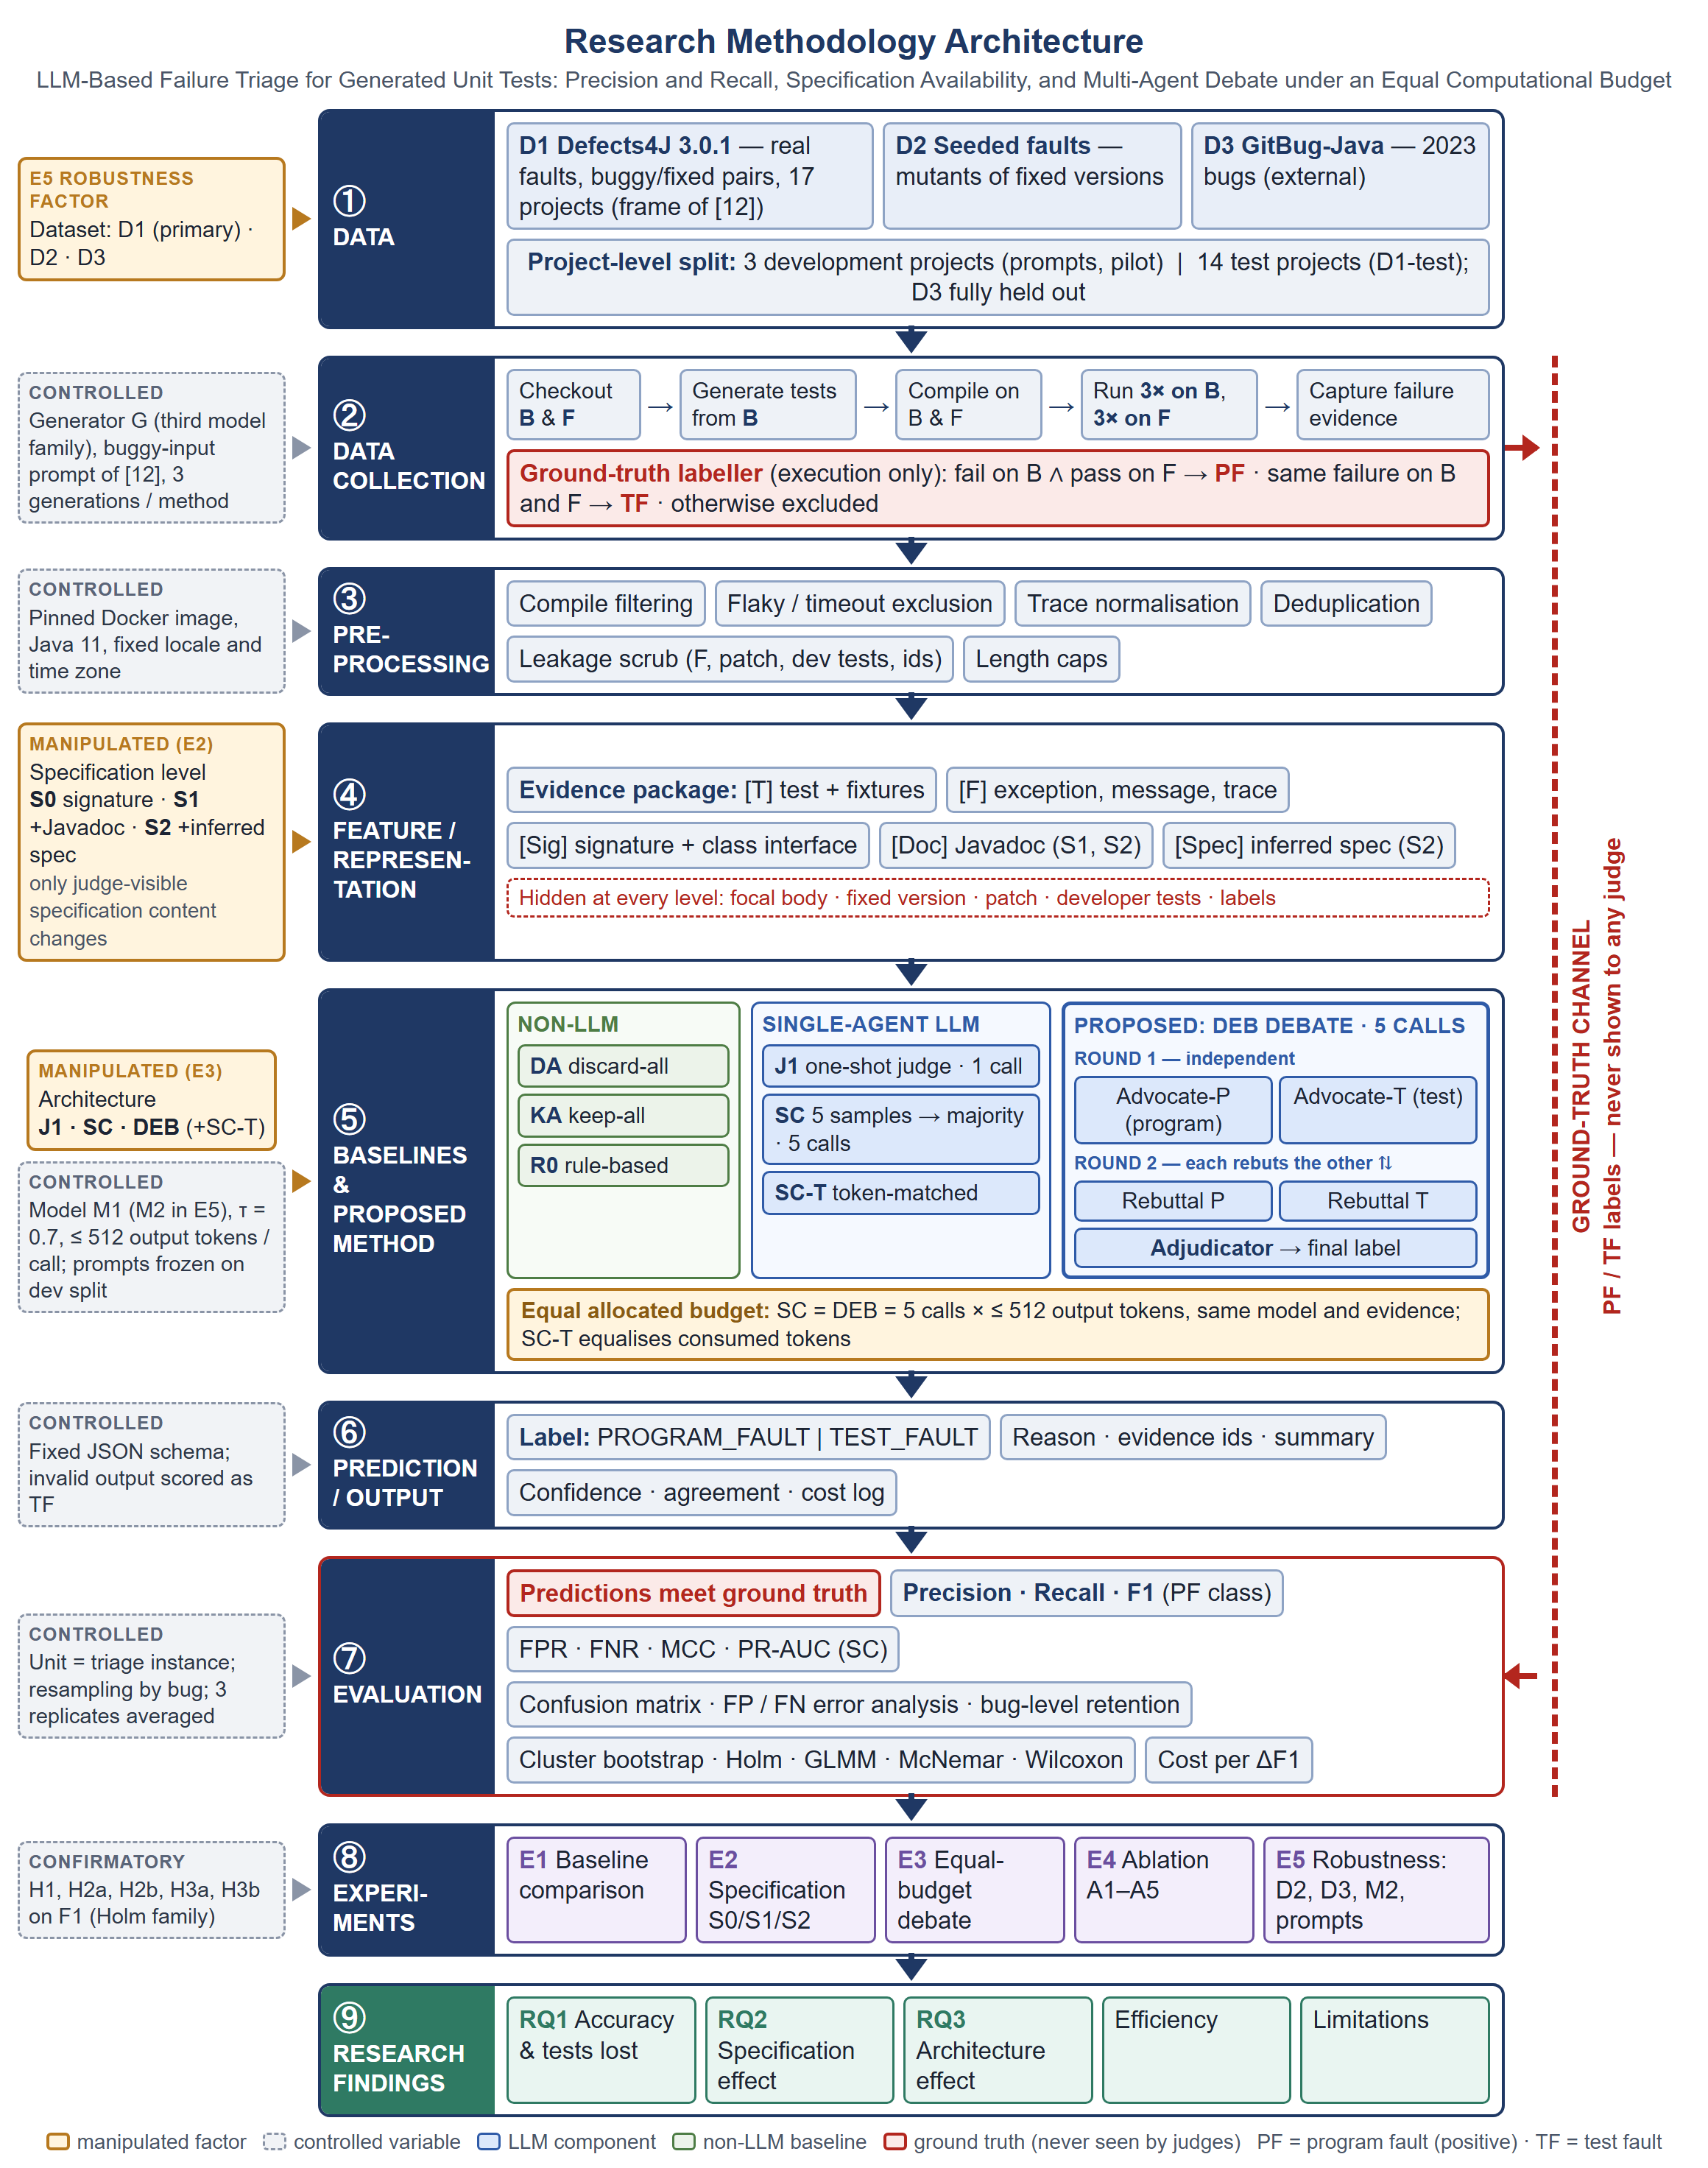
\includegraphics[width=\textwidth,height=0.74\textheight,keepaspectratio]{figures/fig_architecture_phase2.png}
\caption{Research architecture. The central spine is the pipeline; the left lane shows where each factor enters; the right lane is the ground-truth channel, which bypasses every LLM and joins only at evaluation.}\label{fig:arch}
\end{figure*}

\subsection{Ground truth}
Each generated test method is compiled against both versions, in its own copy of the test class, and executed three times on each, every run in a fresh JVM with a timeout. The failure signature $\sigma(t,V)$ on version $V$ is the triple of outcome type, exception class and the test line where the failure surfaced; an outcome is deterministic when all three runs share $\sigma$. Table~\ref{tab:labels} gives the labelling rule. Labels are computed before any judge runs and are stored where no judging module can read them.

\begin{table}[t]
\caption{Ground-truth labelling rule; outcomes must be deterministic over three runs (precedence NC $>$ TIMEOUT $>$ ENV $>$ FLAKY $>$ other rows).}\label{tab:labels}
\footnotesize
\begin{tabularx}{\columnwidth}{@{}l l Y@{}}
\toprule
On $P_B$ & On $P_F$ & Label and use \\
\midrule
fail & pass & \PF{} --- positive class \\
fail & fail, $\sigma_B=\sigma_F$ & \TF{} --- negative class \\
fail & fail, $\sigma_B\neq\sigma_F$ & AMB --- sensitivity analysis only \\
pass & fail or pass & not a triage instance \\
other & --- & FLAKY, TIMEOUT, ENV, NC --- excluded \\
\bottomrule
\end{tabularx}
\end{table}

\subsection{Evidence package and specification levels}
The context builder produces a fixed-format package in which every item carries an identifier that outputs must cite: test lines $[T_i]$, failure items $[F_1]$ (outcome and exception), $[F_2]$ (message with expected/actual values), $[F_3]$ (failing test line) and $[F_{4\ldots}]$ (normalised stack frames), interface items $[\mathit{Sig}_i]$, Javadoc $[\mathit{Doc}_i]$ and specification fields $[\mathit{Spec}_i]$. The levels are nested: S0 $=[T]+[F]+[\mathit{Sig}]$, S1 adds the Javadoc of $P_B$, and S2 adds a specification inferred once per focal method from the signature, Javadoc, call sites and sibling documentation, with lines changed by the fix removed. The focal implementation, the fixed version, the patch, developer tests, bug identifiers and labels are never shown. A leakage guard checks every package against per-instance forbidden strings (bug identifiers, fixed-only lines, focal-body lines, paths) and blocks the call on a match.

\subsection{Triage arms}
All LLM arms use the same model, decoding parameters and evidence package (Table~\ref{tab:arms}). Self-consistency takes the majority of independent samples with ties resolved to \TF; its vote share $v=\#\PF/k$ is kept as a score. The adversarial debate uses exactly five calls (Algorithm~\ref{alg:deb}).

\begin{table}[t]
\caption{Baselines and LLM arms.}\label{tab:arms}
\footnotesize
\begin{tabularx}{\columnwidth}{@{}l c X@{}}
\toprule
Arm & Calls & Decision \\
\midrule
DA & 0 & policy: \TF{} for every instance (discard-all, the practice of repair-first generators) \\
KA & 0 & policy: \PF{} for every instance (keep-all) \\
R0 & 0 & rule: \PF{} iff the failure is not an assertion failure and the deepest project frame is in main code \\
J1 & 1 & one agent: one neutral judgement \\
SC & 5 & one agent: majority of five samples of the J1 prompt \\
SC-T & $k_T$ & one agent: majority of $k_T$ independent samples; $k_T$ = smallest odd $k$ whose consumed tokens reach DEB's on the development split \\
DEB & 5 & multi-agent: adjudicator decision after two rounds of adversarial argument \\
\bottomrule
\end{tabularx}
\end{table}

\begin{algorithm}[t]
\caption{Adversarial debate (DEB) for one instance}\label{alg:deb}
\begin{algorithmic}[1]
\Require evidence package $x$, replicate $r$
\State $a_P^{(1)} \gets \mathrm{LLM}(\textsc{AdvocateP}(x))$; \quad $a_T^{(1)} \gets \mathrm{LLM}(\textsc{AdvocateT}(x))$ \Comment{independent}
\State $a_P^{(2)} \gets \mathrm{LLM}(\textsc{Rebut}(x, a_P^{(1)}, a_T^{(1)}))$; \quad $a_T^{(2)} \gets \mathrm{LLM}(\textsc{Rebut}(x, a_T^{(1)}, a_P^{(1)}))$
\State $\pi \gets$ seeded random order of the two sides, renamed ``Analyst X/Y''
\State $d \gets \mathrm{LLM}(\textsc{Adjudicate}(x, \pi))$ \Comment{decide from cited evidence only}
\State \Return label of $d$ (\textsc{invalid} if $d$ fails schema validation); log position bias and uncited decisions
\end{algorithmic}
\end{algorithm}

\paragraph{Budget accounting and output.} SC and DEB share an allocated budget of five calls; DEB necessarily consumes more input, because Round~2 forwards arguments and the adjudicator reads four. SC-T tests whether a debate advantage survives equal consumed tokens. Every arm emits a JSON record with label, reason category, cited evidence ids, a short summary and a descriptive confidence; one deterministic repair parse is attempted, and outputs that remain invalid are scored as \TF{} in the primary analysis and excluded in a sensitivity analysis. KUU and the cascade (Section~\ref{sec:cascade}) keep a test on an invalid vote, since only positive evidence of a test fault may discard it; scoring the single-judge arms that way changed their balanced accuracy by at most \V{der:inv keep max dBA@3} (Appendix~\ref{app:revision}).

\subsection{Keep-unless-unanimous with disagreement escalation}\label{sec:cascade}
The measured arms lose bug-revealing tests, so we add a triage rule built on three principles. \emph{Keep by default}: a missed bug costs more than a false alarm. \emph{Discard only on cross-family agreement}: judges from different model families should err on different instances, so their unanimity is stronger evidence than repeated samples of one model (we measure this \emph{error diversity} in Section~\ref{sec:kuu}). \emph{Escalate disagreement}: pay for a stronger judge only where the cheap ones disagree. Tier~1 takes one J1 vote from each of M1, M2 and M3 (Ministral~3 14B, a third family); unanimous \TF{} discards and unanimous \PF{} keeps. Tier~2 sends any disagreement, including an invalid vote, to the frontier judge's DEB (Sonnet~5.5, Appendix~\ref{app:post}), whose valid label decides; a missing or invalid answer keeps the test. Tier~1 alone, discarding only on unanimous \TF{}, is KUU. KUU has no tuned parameter: debate's confidence-100 rule set its threshold on the development split, while nothing in KUU was fitted to data. It is a safety rule, not a better classifier. The cascade applies the deferral and selective-prediction patterns~\cite{chen2023frugalgpt,geifman2017selective} to failure triage and is local-first: only escalated failures leave the machine, so for every other failure the source code, failing test, stack trace and message stay on the developer's machine, which matters where code may not be sent to a third-party service. Local compute is not free; it is reported in GPU-seconds and not priced. JSTestCraft also asks three LLMs~\cite{liu2026jstestcraft}, but there a majority out-votes a dissenting judge; unanimity treats dissent as a reason to keep. KUU also requires different families, counts every call in its budget and is scored against execution labels. The cascade and its hypotheses were fixed in advance in the version-controlled decision log before any frontier call on D2, so its D2 result is a test fixed in advance (not externally registered) and its D1 result is post hoc.

%% =====================================================================================
\section{Experimental Setup}\label{sec:setup}

\paragraph{Data and splits.} \textbf{D1 (real faults).} Defects4J~3.0.1 provides, for each real fault, a buggy and a fixed revision~\cite{just2014defects4j,defects4j301}. The sampling frame follows Zhao et al.~\cite{zhao2026misguidance}: methods changed by the fix that exist in both versions, are public or protected and are invoked by a bug-triggering developer test. Their final list is not distributed, so the frame was reconstructed by re-running their selection rule with their replication package~\cite{zhao2026replication}: \V{split:candidates} candidate methods were screened and \V{split:frame_methods} focal methods from \V{split:frame_bugs} defects were kept (the original reports \V{split:reference_frame_zhao:methods} from \V{split:reference_frame_zhao:bugs}). A per-project cap of \V{split:per_project:Lang:sampled} methods leaves \V{split:sampled_methods} focal methods from \V{split:sampled_bugs} defects. A seeded draw, made before any test was generated, placed three projects (\V{der:dev methods} methods) in the development split and \V{der:n test projects} projects (\V{der:test methods} methods) in the held-out split. \textbf{D2 (seeded faults)}, a contamination control, applies one killed mutant inside a held-out focal method of the fixed version: \V{d2rep:before_cap:d2_units_total} mutants yielded \V{d2rep:before_cap:labelled_instances:PF} \PF, \V{d2rep:before_cap:labelled_instances:TF} \TF{} and \V{d2rep:before_cap:labelled_instances:AMB} AMB instances. \textbf{D3} (GitBug-Java~\cite{silva2024gitbug}) was not run, because its build reproduction requires Docker, which was unavailable.

\paragraph{Generation and labels.} The generator produced three generations per focal method from the buggy context. Across both D1 splits, \V{ds1:executed_methods} generated test methods were executed; \V{ds1:exclusions:PASS} passed on the buggy version, \V{ds1:exclusions:MISGUIDED} were misguided (pass on $P_B$, fail on $P_F$) and \V{ds1:exclusions:NC} did not compile on one version. The held-out split yielded \V{der:d1 test PF labelled} \PF, \V{der:d1 test TF labelled} \TF{} and \V{der:d1 test AMB labelled} AMB instances.

\paragraph{Evaluation sample.} Every \PF{} instance is kept and \TF{} instances are sampled at random, stratified by project, so that the sample holds twice as many \TF{} as \PF{} over the split, with inverse-probability weights for prevalence-adjusted precision (the original design did not say whether the ratio holds within projects or overall; the overall reading was fixed before any held-out data existed). The judged D1 sample has \V{sum:prevalence:judged_sample_prevalence_by_dataset:D1:PF} \PF, \V{sum:prevalence:judged_sample_prevalence_by_dataset:D1:TF} \TF{} and \V{sum:prevalence:judged_sample_prevalence_by_dataset:D1:AMB} AMB instances. The D2 sample follows the same rule, capped at \V{d2rep:judged_sample:cap} judged instances: \V{sum2:prevalence:judged_sample_prevalence_by_dataset:D2:PF} \PF, \V{sum2:prevalence:judged_sample_prevalence_by_dataset:D2:TF} \TF{} and \V{sum2:prevalence:judged_sample_prevalence_by_dataset:D2:AMB} AMB; because D2 has fewer \TF{} than twice its \PF, its scored-set \PF{} prevalence (AMB and leakage aborts excluded) is \V{sum2:prevalence:pf_prevalence} against \V{sum:prevalence:pf_prevalence} on D1. The leakage guard aborted \V{sum:leakage_abort_exclusions:counts_labelled:S1|full:instances} D1 instances at S1; following a rule fixed before any result was computed, an instance aborted at a level is excluded from every arm at that level, leaving \V{sum:leakage_abort_exclusions:n_per_level:S1} scored instances at S1 and \V{d2:DEB|S1:n_instances} on D2.

\paragraph{Model selection and configuration.} All models were open-weight and served locally by Ollama~\V{frozen:runtime:version}~\cite{ollama04013} on one laptop GPU (\V{frozen:hardware:name}, \V{frozen:hardware:mem_total_mib@0}\,MiB; \V{frozen:hardware:ram_total_gib@0}\,GB RAM), so no API cost was incurred. They replace the API-served models of the original design (a DeepSeek-V3-family judge, a Qwen3-family judge and GPT-4.1), which were withdrawn before any paid call. Every choice used the development split only. The generator G, Gemma~4 26B-A4B~\cite{gemma4} (\texttt{\V{frozen:roles:G}}, Q4\_K\_M), was selected by criteria fixed in advance: compile-and-execute reliability \V{gsel:C1} (95\% CI \V{gsel:C1_ci95}), fixed-version assertion validity \V{gsel:C2} and program-fault yield \V{gsel:P1@pct}, above the original design's yield floor of \V{gsel:thresholds:P1@pct0}. The primary judge M1 is the candidate from the other family, Qwen3.5 9B~\cite{qwen35_9b} (\texttt{\V{frozen:roles:M1}}); the robustness judge M2 is Gemma~4 12B (\texttt{\V{frozen:roles:M2}}), which shares a family with G. On a \V{devgate:n_instances}-instance, \V{devgate:n_bugs}-bug development pilot, M1 passed the output-validity and evidence-citation gates but \emph{failed} the gate requiring its one-shot F1 to exceed both trivial baselines: F1 \V{devgate:G_d_detail:J1_f1} (MCC \V{devgate:G_d_detail:J1_mcc}) against \V{devgate:G_d_detail:R0_f1} (MCC \V{devgate:G_d_detail:R0_mcc}) for R0. The failure persisted over five prompt rounds, an 8-bit quantisation and the other family, and an audit found no pipeline defect, so M1 was kept and the failure is reported. M2, M3 and the fourth-family judge of Section~\ref{sec:kuu} failed the same gate (Appendix~\ref{app:revision}): every local judge in this study is below its own development gate, so a null result here describes these judges, not the architectures or specifications in general. Thinking modes were disabled. All judge calls used temperature \V{frozen:frozen_models:M1:temperature:judges@1}, top-$p$ \V{frozen:frozen_models:M1:top_p@1}, a context of \V{frozen:frozen_models:M1:num_ctx@int} tokens, at most \V{frozen:frozen_models:M1:num_predict:judge_roles} output tokens and a per-call seed; the specification inferencer used temperature \V{frozen:frozen_models:M1:temperature:spec_inferencer@0}. Repeating \V{nondet:n} development judgements with identical seeds flipped \V{nondet:T0.7:label_flip_rate@pct0} of labels. Runtime, digests, server settings, decoding, seeds and prompt hashes were frozen in one file before any held-out call; $k_T$ was fixed at \V{frozen:decoding:k_T} on the development split, so SC-T uses SC's configuration with independently drawn samples.

\paragraph{Experiments.} E1--E3 (all arms, S0--S2, \V{frozen:decoding:replicates} replicates, SC-T at S1) use M1 on D1-test; E4 (ablations, one replicate) uses M1 on D1-test; E5 adds D2 with M1 (all arms and levels, one replicate), M2 on D1-test and D2 (J1, SC, DEB at S1, one replicate), and an exploratory larger judge (Section~\ref{sec:robust}). Builds and executions ran on Ubuntu~22.04.5 under WSL2 with OpenJDK~11 and Defects4J~3.0.1; analysis used Python with NumPy, SciPy and statsmodels~\cite{seabold2010statsmodels}. \TODO{public repository URL and archived artefact DOI.}

\paragraph{Metrics and statistics.} Precision, recall and F1 of the \PF{} class, MCC~\cite{chicco2020mcc}, the \PF{}-retention rate TPR $=\mathrm{TP}/(\mathrm{TP}+\mathrm{FN})$, the \TF{}-removal rate TNR $=\mathrm{TN}/(\mathrm{TN}+\mathrm{FP})$ and balanced accuracy (TPR+TNR)/2, which, unlike F1 and MCC, do not move with the \PF{}:\TF{} mix, FPR, confusion matrices, \PF{} tests lost, precision at the natural prevalence (inverse sampling weights), and invalid-output rate. Metrics are computed per replicate and averaged; 95\% CIs come from a 10{,}000-resample bug-level cluster bootstrap~\cite{efron1993bootstrap}, with identical resamples for paired differences; a bootstrap $p$ is two-sided, twice the smaller share of resampled differences on either side of zero (+1 corrected). These intervals hold the replicate mean fixed, so decoding noise is not in them (Table~\ref{tab:noise} gives M1's run-to-run range). The five confirmatory F1 tests (H1: J1 vs R0; H2a: S1 vs S0 on methods with Javadoc; H2b: S2 vs S1; H3a: DEB vs SC; H3b: SC vs J1; at S1 unless stated) are Holm-corrected~\cite{holm1979}, with recall and precision as a secondary Holm family; equivalence is declared when the 90\% CI lies within $\pm0.05$ F1~\cite{lakens2017equivalence}. McNemar's exact test~\cite{dietterich1998tests}, per-project Wilcoxon tests~\cite{wilcoxon1945} and leave-one-project-out re-estimation are sensitivity analyses~\cite{arcuri2011guide}. A hypothesis described as fixed in advance was written into the version-controlled decision log before its calls; that is internal provenance, not an external, time-stamped preregistration. Analyses added in response to review are post hoc or exploratory (Appendix~\ref{app:revision}).

%% =====================================================================================
\section{Results and Analysis}\label{sec:results}

\subsection{RQ1: triage accuracy against ground truth (E1)}
Table~\ref{tab:e1} (Figure~\ref{fig:prf} in Appendix~\ref{app:extra}) reports all arms at S1 on the \V{sum:leakage_abort_exclusions:n_per_level:S1} scored D1-test instances (\PF{} prevalence \V{sum:prevalence:pf_prevalence}). Keep-all reaches F1 \V{d1:KA:f1} with MCC \V{d1:KA:mcc}, so F1 alone would rank a constant answer level with the best LLM arm. Every LLM arm has a positive MCC, the rule baseline a negative one (\V{d1:R0:mcc}). DEB has the highest F1 (\V{d1:DEB|S1:f1}) and MCC (\V{d1:DEB|S1:mcc}) of the arms in Table~\ref{tab:e1}; its F1 exceeds keep-all's by only \V{der:d1 DEB-KA f1}, and its MCC interval excludes zero. Of the \V{sum:prevalence:PF} bug-revealing tests, DEB discards \V{d1:DEB|S1:pf_lost@0} and SC \V{d1:SC|S1:pf_lost@0} per replicate (DEB recall \V{d1:DEB|S1:recall}), R0 \V{d1:R0:pf_lost@0} and discard-all all \V{d1:DA:pf_lost@0}. At the natural prevalence, DEB's precision falls to \V{d1:DEB|S1:precision_prev_adj}: most kept tests would still be test faults. Invalid outputs were rare (at most \V{d1:J1|S1:invalid_rate@pct} for J1).

\begin{table*}[t]
\caption{E1: baselines and LLM arms at S1, D1-test, judge M1 (mean of \V{frozen:decoding:replicates} replicates for LLM arms). $P_\mathrm{adj}$: precision at the natural prevalence. Lost: \PF{} tests classified \TF. Inv.: invalid-output rate. CIs: bug-level cluster bootstrap.}\label{tab:e1}
\footnotesize\setlength{\tabcolsep}{3.5pt}
\begin{tabular}{@{}l c c c c c c c@{}}
\toprule
Arm & F1 [95\% CI] & MCC [95\% CI] & P & R & $P_\mathrm{adj}$ & Lost & Inv. \\
\midrule
DA & \V{d1:DA:f1} & \V{d1:DA:mcc} & n/a & \V{d1:DA:recall} & n/a & \V{d1:DA:pf_lost} & -- \\
KA & \V{d1:KA:f1} \V{d1:KA:f1_ci95} & \V{d1:KA:mcc} & \V{d1:KA:precision} & \V{d1:KA:recall} & \V{d1:KA:precision_prev_adj} & \V{d1:KA:pf_lost} & -- \\
R0 & \V{d1:R0:f1} \V{d1:R0:f1_ci95} & \V{d1:R0:mcc} \V{d1:R0:mcc_ci95} & \V{d1:R0:precision} & \V{d1:R0:recall} & \V{d1:R0:precision_prev_adj} & \V{d1:R0:pf_lost} & -- \\
J1 & \V{d1:J1|S1:f1} \V{d1:J1|S1:f1_ci95} & \V{d1:J1|S1:mcc} \V{d1:J1|S1:mcc_ci95} & \V{d1:J1|S1:precision} & \V{d1:J1|S1:recall} & \V{d1:J1|S1:precision_prev_adj} & \V{d1:J1|S1:pf_lost@1} & \V{d1:J1|S1:invalid_rate@pct} \\
SC & \V{d1:SC|S1:f1} \V{d1:SC|S1:f1_ci95} & \V{d1:SC|S1:mcc} \V{d1:SC|S1:mcc_ci95} & \V{d1:SC|S1:precision} & \V{d1:SC|S1:recall} & \V{d1:SC|S1:precision_prev_adj} & \V{d1:SC|S1:pf_lost@1} & \V{d1:SC|S1:invalid_rate@pct} \\
SC-T & \V{d1:SC-T|S1:f1} \V{d1:SC-T|S1:f1_ci95} & \V{d1:SC-T|S1:mcc} \V{d1:SC-T|S1:mcc_ci95} & \V{d1:SC-T|S1:precision} & \V{d1:SC-T|S1:recall} & \V{d1:SC-T|S1:precision_prev_adj} & \V{d1:SC-T|S1:pf_lost@1} & \V{d1:SC-T|S1:invalid_rate@pct} \\
DEB & \V{d1:DEB|S1:f1} \V{d1:DEB|S1:f1_ci95} & \V{d1:DEB|S1:mcc} \V{d1:DEB|S1:mcc_ci95} & \V{d1:DEB|S1:precision} & \V{d1:DEB|S1:recall} & \V{d1:DEB|S1:precision_prev_adj} & \V{d1:DEB|S1:pf_lost@1} & \V{d1:DEB|S1:invalid_rate@pct} \\
\bottomrule
\end{tabular}
\end{table*}


H1 (J1 vs R0) gives $\Delta$F1 \V{conf:f1:H1:delta} (95\% CI \V{conf:f1:H1:ci95}), $p$ \V{conf:f1:H1:p} and $p_\mathrm{Holm}$ \V{conf:f1:H1:p_holm}; the 95\% interval just includes zero and the 90\% interval (\V{conf:f1:H1:ci90}) does not, so the result is inconclusive at this sample size. McNemar's test agrees ($p$ \V{sum:mcnemar:H1:p}), and the per-project Wilcoxon test over the \V{sum:wilcoxon_projects:H1:n_projects} projects with both classes gives $p$ \V{sum:wilcoxon_projects:H1:p}.

\subsection{RQ2: specification availability (E2)}
Table~\ref{tab:e2} (Appendix~\ref{app:extra}) and Figure~\ref{fig:spec} (Appendix~\ref{app:explore}) show F1 by level. No arm improves from S0 to S1: adding Javadoc changed F1 by \V{der:d1 J1 S1-S0 f1} (J1), \V{der:d1 SC S1-S0 f1} (SC) and \V{der:d1 DEB S1-S0 f1} (DEB), and S0 gives the highest F1 and MCC for every arm. On the methods with Javadoc, H2a gives $\Delta$F1 \V{conf:f1:H2a:delta} (95\% CI \V{conf:f1:H2a:ci95}); the interval excludes zero before correction ($p$ \V{conf:f1:H2a:p}) but not after ($p_\mathrm{Holm}$ \V{conf:f1:H2a:p_holm}), and recall shows the same direction ($\Delta$ \V{conf:secondary:H2a~recall:delta}). The inferred specification did not help either: H2b gives $\Delta$F1 \V{conf:f1:H2b:delta} (\V{conf:f1:H2b:ci95}, $p_\mathrm{Holm}$ \V{conf:f1:H2b:p_holm}), and its precision difference (\V{conf:secondary:H2b~precision:delta}, 90\% CI \V{conf:secondary:H2b~precision:ci90}) is practically equivalent to zero. An exploratory mixed model finds no specification effect either (Appendix~\ref{app:explore}).


\subsection{RQ3: equal-budget architectures (E3)}
Table~\ref{tab:e3} (Appendix~\ref{app:extra}; Figure~\ref{fig:pareto}, Appendix~\ref{app:explore}) compares the arms at equal allocated budget. DEB's F1 exceeds SC's by \V{conf:f1:H3a:delta} (H3a, 95\% CI \V{conf:f1:H3a:ci95}, $p_\mathrm{Holm}$ \V{conf:f1:H3a:p_holm}) and SC-T's by \V{sum:sc_t_check:delta} (\V{sum:sc_t_check:ci95}); SC's differs from J1's by \V{conf:f1:H3b:delta} (H3b, \V{conf:f1:H3b:ci95}, $p_\mathrm{Holm}$ \V{conf:f1:H3b:p_holm}). The debate advantage is therefore consistent in direction but not significant, and five samples of the same judge did not improve on one. DEB consumed slightly fewer tokens per instance than SC (\V{d1:DEB|S1:consumed_tokens_per_instance@0} vs \V{d1:SC|S1:consumed_tokens_per_instance@0}), which is why the token-matched $k_T$ equalled SC's five samples, but it took longer (\V{d1:DEB|S1:latency_s_per_instance@1}\,s vs \V{d1:SC|S1:latency_s_per_instance@1}\,s) because its calls are sequential. The adjudicator sided with the analyst presented last in \V{d1:DEB|S1:position_bias_rate@pct} of decisions, and \V{d1:DEB|S1:no_evidence_rate@pct} of its decisions cited no evidence.


Measured from the call logs (Table~\ref{tab:cost}), DEB made \V{cost:arms:DEB:calls_per_instance@0} calls per instance against J1's \V{cost:arms:J1:calls_per_instance@0}, consumed \V{cost:deb_over_j1:tokens@1} times its tokens and \V{cost:deb_over_j1:median_wall@1} times its median wall time (\V{cost:arms:DEB:wall_s_median@1}\,s vs \V{cost:arms:J1:wall_s_median@1}\,s) for an F1 gain over J1 of \V{der:d1 DEB-J1 f1}, a difference no confirmatory test covers.

\subsection{Confirmatory tests}
Table~\ref{tab:conf} and Figure~\ref{fig:forest} (Appendix~\ref{app:extra}) summarise the confirmatory family; every difference and $p$ is given in the RQ subsections above. No hypothesis is supported after Holm correction, and none is shown to be practically equivalent; all five are inconclusive at this sample size. The secondary recall and precision family gives the same verdict.



\subsection{Robustness (E5)}\label{sec:robust}
Table~\ref{tab:robust} (Appendix~\ref{app:extra}) reports D2 and the second judge. \textbf{Seeded faults (D2).} D2's \PF{} prevalence is \V{sum2:prevalence:pf_prevalence}, so keep-all reaches F1 \V{d2:KA:f1} at MCC \V{d2:KA:mcc}; F1 is not comparable between D1 and D2, and MCC and prevalence-adjusted precision are the cross-dataset measures. Under M1, every LLM arm again has a positive MCC and beats R0 (MCC \V{d2:R0:mcc}); DEB has the highest MCC (\V{d2:DEB|S1:mcc}), but SC's F1 is higher than DEB's by \V{der:d2 SC-DEB f1}. DEB at S2 is the best thinking-disabled D2 cell (F1 \V{d2:DEB|S2:f1}, MCC \V{d2:DEB|S2:mcc}). None of the D2 contrasts that mirror the hypotheses is significant after Holm. In \V{der:d2 aborts mutated line} of the \V{der:d2 aborted instances} aborted D2 instances the guard's match was the injected mutated line itself, a genuine leak that the guard blocked.

\textbf{Second judge (M2).} On the same instances, M2 (12B) improved on M1 in every arm and dataset (DEB on D1-test by \V{r3:D1:m2_minus_m1:DEB:f1:delta}, 95\% CI \V{r3:D1:m2_minus_m1:DEB:f1:ci95}; detail in Appendix~\ref{app:post}); it shares the generator's family, so self-preference cannot be excluded.


\textbf{Further judges.} A 35B and a third-family judge, a three-family vote (one replicate each) and a frontier reference judge (Claude Sonnet~5.5: DEB F1 \V{e9:summary:DEB|S1|SON:f1}, run-to-run range \V{e9:deb_run_to_run_spread:sonnet:f1:range} against M1's \V{e9:deb_run_to_run_spread:m1:f1:range}) are in Appendix~\ref{app:post}; all are robustness evidence.

\subsection{RQ4: keep unless unanimous and disagreement escalation}\label{sec:kuu}
\begin{figure*}[t]
\centering
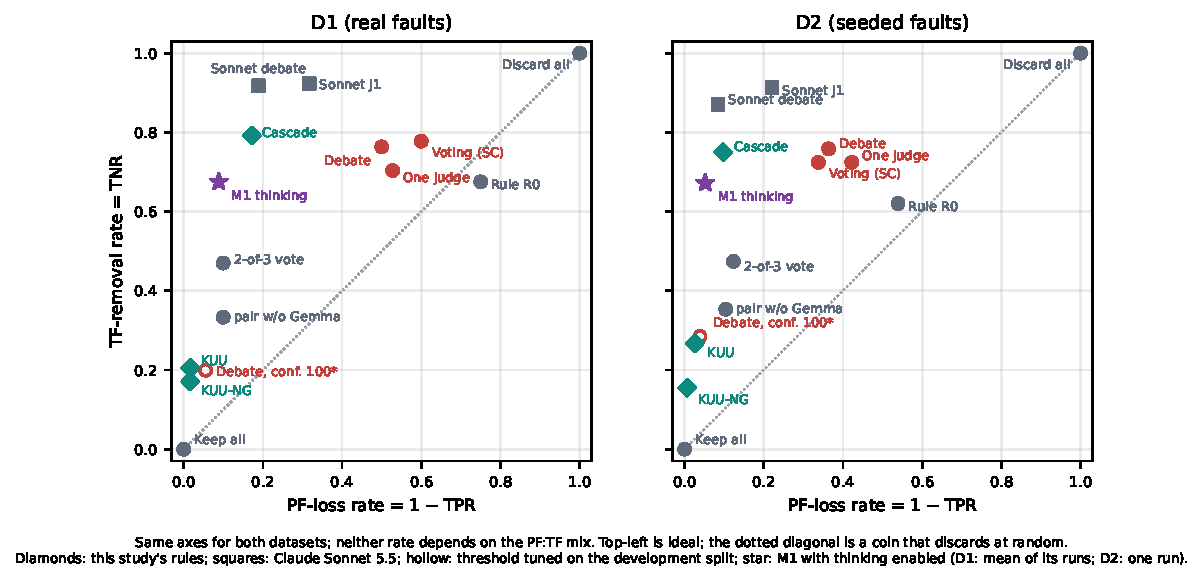
\includegraphics[width=0.66\textwidth]{figures/fig_tradeoff_rates.pdf}
\caption{Every rule on rates that do not depend on the \PF{}:\TF{} mix (post hoc, descriptive): \PF{}-loss rate (1 $-$ TPR) against \TF{}-removal rate (TNR), identical axes for D1-test and D2; top left is best. Diamonds: this study's rules; squares: the frontier judge; hollow: the one threshold tuned on the development split; star: M1's one-shot judge with thinking enabled (D1-test: mean of three runs; D2: the confirmation run; Table~\ref{tab:think}). Figure~\ref{fig:tradeoff} (Appendix~\ref{app:revision}) shows the share discarded against the share lost.}\label{fig:rates}
\end{figure*}
Single-judge arms with thinking disabled discard about half of the bug-revealing tests (DEB \V{d1:DEB|S1:pf_lost@0} of \V{sum:prevalence:PF}), while the cross-family vote lost far fewer. \textbf{KUU} is Tier~1 of Section~\ref{sec:cascade}: discard only on three unanimous \TF{} votes. KUU was defined after the D1 vote (post hoc on D1) and tested once on unseen D2 with its hypotheses fixed in advance. On D1 it lost \V{kuu1:summary:KUU|S1:pf_lost@0} of \V{sum:prevalence:PF} (F1 \V{kuu1:summary:KUU|S1:f1}); on D2, with fresh calls (\V{kuu2:n_instances} instances, \V{kuu2:n_bugs} bugs), it reached F1 \V{kuu2:summary:KUU|S1:f1} against keep-all's \V{kuu2:summary:KA:f1} ($\Delta$F1 \V{kuu2:hypotheses:H10-1:delta} \V{kuu2:hypotheses:H10-1:ci95}, $p_\mathrm{Holm}$ \V{kuu2:hypotheses:H10-1:p_holm}) and lost \V{kuu2:summary:KUU|S1:pf_lost@0} of \V{kuu2:pf_prevalence:PF} bug-revealing tests against DEB's \V{kuu2:summary:DEB|S1:pf_lost@0} (paired, $p_\mathrm{Holm}$ \V{kuu2:hypotheses:H10-2:p_holm}); both are supported, but its MCC (\V{kuu2:summary:KUU|S1:mcc}) is below DEB's (\V{kuu2:summary:DEB|S1:mcc}), so KUU alone is a conservative operating point, not a better classifier. In the discarded-versus-lost view (Figure~\ref{fig:tradeoff}, Appendix~\ref{app:revision}), on D2 KUU discards \V{pareto:D2:points:KUU|S1:share_discarded@pct0} of failures and loses \V{pareto:D2:points:KUU|S1:pf_lost@0} tests, where debate with a confidence-100 threshold, tuned on the development split, discards \V{pareto:D2:points:TAU|S1:share_discarded@pct0} and loses \V{pareto:D2:points:TAU|S1:pf_lost@0}; KUU reaches that point with no tuning. Against the thinking-enabled judge (Table~\ref{tab:think}), KUU still adds protection: of D2's bug-revealing tests, \V{tk:d2:kuu_vs_thinking:pf_lost_by_thinking_kept_by_kuu@int} lost by that judge are kept by KUU and \V{tk:d2:kuu_vs_thinking:pf_lost_by_kuu_kept_by_thinking@int} the reverse, at a cost of removing \V{tk:d2:descriptive:KUU:tnr@pct0} of test faults against its \V{tk:d2:descriptive:ThinkingM1J1:tnr@pct0}.

\textbf{Without the generator's family (KUU-NG).} Without M2, which shares the generator's family, the pair M1 + M3 loses \V{loo:D2:summary:M1_E6B|S1:pf_lost@0} tests rather than \V{kuu2:summary:KUU|S1:pf_lost@0} (Appendix~\ref{app:review}), so KUU's protection might rest on a judge reluctant to fault its sibling's tests. We replaced M2 with a fourth-family judge (Llama~3.1 8B, chosen on the development split by the rules that chose M3) and ran it once with fresh calls. On D2, KUU-NG lost \V{kuung:D2:summary:KUUNG|S1:pf_lost@0} bug-revealing test and no bug entirely, against \V{kuung:D2:summary:DEB|S1:bugs_lost@0} bugs for M1 DEB ($\Delta$ \V{kuung:D2:hypotheses:H13-2:delta@0} \V{kuung:D2:hypotheses:H13-2:ci95@ci0}, $p_\mathrm{Holm}$ \V{kuung:D2:hypotheses:H13-2:p_holm}), and its F1 (\V{kuung:D2:summary:KUUNG|S1:f1}) exceeded keep-all's ($\Delta$F1 \V{kuung:D2:hypotheses:H13-1:delta} \V{kuung:D2:hypotheses:H13-1:ci95}, $p_\mathrm{Holm}$ \V{kuung:D2:hypotheses:H13-1:p_holm}); both hypotheses fixed in advance are supported, and D1 agrees. The new judge is not lenient (\PF{} miss rate \V{kuungm:D2:kuung:NG:miss_rate_on_pf} against M2's \V{kuungm:D2:kuu:M2:miss_rate_on_pf}; post hoc), so the protection does not need a generator-family judge. KUU-NG discards less, though (\V{kuung:D2:summary:KUUNG|S1:share_discarded@pct0} of failures against \V{kuung:D2:summary:KUU|S1:share_discarded@pct0}), and its MCC (\V{kuung:D2:summary:KUUNG|S1:mcc}) is lower than KUU's, not significantly (Appendix~\ref{app:cascade}).

\textbf{Error diversity.} On D2 two families miss the same \PF{} test \V{ed:D2:comparison:mean_cross_family_lift@1} times as often as independence predicts and three samples of one model \V{ed:D2:comparison:mean_within_family_lift@1} times (difference \V{ed:D2:comparison:difference_ci95@ci2}); the diversity is partial, and on D1 (post hoc) the criterion fixed in advance is not met (Appendix~\ref{app:cascade}).

\textbf{Escalating disagreement (fixed in advance on D2).} The cascade sent \V{cas2:escalation:escalated@0} of \V{cas2:n_instances} instances (\V{cas2:escalation:share_escalated@pct0}) to Sonnet's DEB, so the other half of the failures never left the machine. Per instance its local tier used \V{pareto:D2:points:CAS|S1:local_gpu_s_per_instance@1} GPU-seconds on one laptop GPU and its frontier tier US\$\,\V{pareto:D2:points:CAS|S1:frontier_usd_per_instance@3}; Sonnet's DEB on every instance cost US\$\,\V{pareto:D2:points:DEB|S1|SON:frontier_usd_per_instance@3} and sends every failure off the machine. Its MCC rose to \V{cas2:summary:CAS|S1:mcc} from KUU's \V{cas2:summary:KUU|S1:mcc} ($\Delta$MCC \V{cas2:hypotheses:H12-1:delta} \V{cas2:hypotheses:H12-1:ci95}, $p_\mathrm{Holm}$ \V{cas2:hypotheses:H12-1:p_holm}, supported), but its F1 (\V{cas2:summary:CAS|S1:f1}) against Sonnet's DEB on every instance (\V{cas2:summary:DEB|S1|SON:f1}) gave $\Delta$ \V{cas2:hypotheses:H12-2:delta}, 95\% CI \V{cas2:hypotheses:H12-2:ci95}: non-inferiority at $-0.05$ is \emph{not} shown ($p_\mathrm{Holm}$ \V{cas2:hypotheses:H12-2:p_holm}). It lost \V{cas2:summary:CAS|S1:pf_lost@0} bug-revealing tests (KUU \V{cas2:summary:KUU|S1:pf_lost@0}, Sonnet \V{cas2:summary:DEB|S1|SON:pf_lost@0}). Escalation thus recovers most of the frontier judge's accuracy, not all of it, while keeping half of the evidence local; Sonnet J1 on every instance reaches a similar MCC but sends every failure off the machine and leaves more bugs uncovered (Appendix~\ref{app:review}). D1 (post hoc) agrees (Appendix~\ref{app:cascade}). \textbf{Fully local (post hoc).} With the thinking-enabled M1 judge as Tier~2, so that no failure leaves the machine, the cascade lost \V{lc:D2:runs:62:local_cascade:pf_lost@0} bug-revealing tests and \V{lc:D2:runs:62:local_cascade:bugs_lost@0} bugs on D2 against the Sonnet cascade's \V{lc:D2:comparators:Sonnetcascade:pf_lost@0} and \V{lc:D2:comparators:Sonnetcascade:bugs_lost@0}, but removed fewer test faults (balanced accuracy \V{lc:D2:runs:62:local_cascade:ba} against \V{lc:D2:comparators:Sonnetcascade:ba}); it was defined after D2 was seen and awaits fresh data (Table~\ref{tab:localcas}).

\textbf{Rates, ranking and trained baselines (post hoc).} On mix-independent rates (Figure~\ref{fig:rates}) KUU's balanced accuracy (\V{rv11:D2:rules:KUU|S1:ba}) is below debate's (\V{rv11:D2:rules:DEB|S1:ba}) and the cascade's (\V{rv11:D2:rules:CAS|S1:ba}); the held-out test faults, ranking and trained baselines are in Appendix~\ref{app:extra}.

%% =====================================================================================
\section{Comparison with Base Papers and State of the Art}\label{sec:comparison}

\paragraph{Summary.} Table~\ref{tab:base} (Appendix~\ref{app:extra}) summarises the ten base papers: authors and year, problem, method, data, metrics and reported results. All reported results are the original authors' (*).


\paragraph{Quantitative comparison.} Only JSTestCraft reports a triage metric (audited recall~\cite{liu2026jstestcraft}); JavaOracle reports a precision~\cite{fu2026javaoracle}. Table~\ref{tab:quant} (Appendix~\ref{app:extra}) lists both, marked *, beside our methods on identical D1-test instances: discard-all re-implements repair-first generators~\cite{gu2026testart,hayet2025chatassert}, R0 rule-based triage~\cite{maddila2026agentic,herzig2015alarms}, and VOTE3 a three-family majority vote in JSTestCraft's manner with local judges; SC is its single-model, equal-budget analogue.


\paragraph{Improvement analysis.} On identical instances DEB's F1 exceeds R0's, SC's and J1's, none significantly after Holm, and keep-all's by only \V{der:d1 DEB-KA f1}; the real gain over keep-all is in MCC (\V{d1:DEB|S1:mcc} vs \V{d1:KA:mcc}). No improvement over a base paper can be computed: none reports a triage result on this data, metric or label source, so the two published figures are context, not targets. The full comparison, why the numbers differ, the fairness of the comparison, re-implementation fidelity and the methodological comparison are in Appendix~\ref{app:extra}.

%% =====================================================================================
\section{Ablation Study}\label{sec:ablation}

Each ablation changes one component of a full arm and is compared with that parent on identical instances (Table~\ref{tab:abl} and Figure~\ref{fig:abl} in Appendix~\ref{app:extra}); debate ablations keep the five-call budget. Ablations are exploratory (one replicate, no multiplicity correction).



\textbf{Failure evidence (A4)} is the only component whose removal has a clear effect: without it, F1 drops for every arm, by \V{abl:SC|S1|noF-SC|S1:delta} for SC (95\% CI \V{abl:SC|S1|noF-SC|S1:ci95}) and \V{abl:J1|S1|noF-J1|S1:delta} for J1, and MCC falls to \V{d1:SC|S1|noF:mcc} (SC) and \V{d1:J1|S1|noF:mcc} (J1), i.e.\ chance; DEB's F1 also dropped (\V{abl:DEB|S1|noF-DEB|S1:delta}, 95\% CI \V{abl:DEB|S1|noF-DEB|S1:ci95}, $p$ \V{abl:DEB|S1|noF-DEB|S1:p}), though not significantly, and its MCC stayed at \V{d1:DEB|S1|noF:mcc}. The judge's signal therefore comes from the execution evidence, which also argues against decisions recalled from a memorised benchmark. \textbf{Debate components (A1, A2)} do not help: removing the exchange of arguments or the adversarial roles left F1 slightly higher (\V{abl:A1|S1-DEB|S1:delta}, \V{abl:A2|S1-DEB|S1:delta}), with intervals that include zero, so the debate's small advantage is not attributable to adversarial argument. \textbf{Aggregation (A3)}: lowering SC's threshold to two of five votes raised recall to \V{sum:A3:SC|S1|A3 v>=2/5:recall} and F1 to \V{sum:A3:SC|S1|A3 v>=2/5:f1}, above every full arm at S1; requiring four of five cut recall to \V{sum:A3:SC|S1|A3 v>=4/5:recall}. \textbf{Implementation (A5)}: showing the buggy body changed F1 by \V{abl:J1|S1|impl-J1|S1:delta} (J1) and \V{abl:DEB|S1|impl-DEB|S1:delta} (DEB), neither significant, and a body-derived specification by \V{abl:J1|S2|specprime-J1|S2:delta}.

%% =====================================================================================
\section{Discussion}\label{sec:discussion}

\paragraph{Failure evidence matters.} The clearest (exploratory) result is A4: without the failure section, J1 and SC fell to chance and DEB's F1 also dropped, though not significantly. Triage stages should pass the complete failure (message with expected and actual values, failing line, project frames) to the judge; it is also the cheapest part of the package to build.

\paragraph{Debate and Javadoc: inconclusive.} Among the thinking-disabled arms, DEB has the highest MCC in all four dataset--judge combinations (Table~\ref{tab:robust}), but H3a is not significant ($p_\mathrm{Holm}$ \V{conf:f1:H3a:p_holm}) and the ablations attribute none of it to adversarial argument. Javadoc lowered F1 for every arm, but H2a does not survive Holm and its interval includes zero once replicates are resampled (Appendix~\ref{app:review}). Both effects are inconclusive: differences smaller than the design's MDE cannot be excluded, and every local judge failed its own development gate, so these nulls describe weak judges, not the factors.

\paragraph{Test-time reasoning versus orchestration.} With thinking enabled, one M1 call beat M1's five-call debate on D2 ($\Delta$MCC \V{tk:d2:confirmatory:HT-1:delta} \V{tk:d2:confirmatory:HT-1:ci95}, $p_\mathrm{Holm}$ \V{tk:d2:confirmatory:HT-1:p_holm}; \V{tk:d2:confirmatory:HT-2:pf_lost_thinking@int} against \V{tk:d2:confirmatory:HT-2:pf_lost_deb@int} bug-revealing tests lost; the verdict holds whichever way the \V{tk:d2:capped@int} outputs cut off by the cap are scored) and every planned M1 arm on D1-test in each of three runs (balanced accuracy \V{tk:d1:summary:ba:min}--\V{tk:d1:summary:ba:max}), on fewer tokens per instance than debate (\V{tk:d1:summary:tokens_per_instance:mean@0} against \V{tk:deb_tokens_per_instance_D1@0}; not token-matched). For small judges, then, the gain RQ3 looked for in orchestration came instead from reasoning inside one call. It is not a validated judge: it failed its development gate on \V{tk:gate:n_instances@int} pilot instances (F1 \V{tk:gate:G_d_detail:J1_f1} against R0's \V{tk:gate:G_d_detail:R0_f1}; \V{tk:gate:G_a_valid_rate:J1@pct1} valid outputs against the 98\% required), the 12B M2's debate scored about as high on D1-test (MCC \V{d1m2:DEB|S1:mcc} against \V{tk:d1:summary:mcc:min}--\V{tk:d1:summary:mcc:max} over three runs), and it lost more bug-revealing tests than KUU, so it is a stronger classifier, not a safety rule (Table~\ref{tab:think}).

\paragraph{Practical value of KUU is limited.} Its F1 gain over keep-all is small (\V{kuu2:hypotheses:H10-1:delta}; KUU-NG \V{kuung:D2:hypotheses:H13-1:delta}), and at a 5\% \PF{} prevalence a developer would still read about \V{rv11:D2:rules:KUU|S1:at_prevalence:0.0500:false_alarms_per_kept_pf@0} test faults per bug-revealing test kept (\V{rv11:D2:rules:KA:at_prevalence:0.0500:false_alarms_per_kept_pf@0} untriaged). It suits settings where a lost bug costs far more than a false alarm; ranking with deferral may serve developers better (Appendix~\ref{app:revision}), and bugs still detected after triage and repair are not measured.








\paragraph{Were the gaps and objectives met?} G1: triage is measured against execution labels; the confirmatory effects are inconclusive at this size. G2: specifications gave no gain. G3: the equal-budget debate advantage is small and not significant. RQ4: KUU cut lost bug-revealing tests without lowering F1, with or without a generator-family judge; escalation recovered MCC but not the frontier judge's F1.

\subsection{Limitations, deviations and threats to validity}
\textit{Construct.} The fixed version is an operational reference, not proof of correctness~\cite{zhao2026misguidance}; AMB double failures are excluded, and including them as \PF{} or \TF{} moved DEB's F1 to \V{sum:sensitivity_f1:AMB_as_PF:DEB|S1:f1} or \V{sum:sensitivity_f1:AMB_as_TF:DEB|S1:f1}. A two-rater blind audit of \V{aud:n_items} development-split instances (all \V{aud:labels:PF} \PF{} and \V{aud:labels:TF} of \V{aud:dev_split_labels:TF} \TF{}, none held out) gave Cohen's $\kappa$~\cite{cohen1960kappa} \V{aud2:raters:kappa} between the raters (95\% bug-level CI \V{aud2:raters:kappa_ci95_bug_bootstrap}); their consensus matched the execution label on \V{aud2:consensus_vs_execution:agreement@pct1} of items ($\kappa$ \V{aud2:consensus_vs_execution:kappa_pf_tf}), and both mismatches were execution \TF{} that the raters judged \PF{}. The raters are the authors, saw the developer's fix and rated development-split instances only; the audit still tests the rule, which is mechanical and identical on both splits. A sealed LLM third rater agreed with the human consensus at $\kappa$ \V{aud2:llm_rater_secondary_D84:consensus_vs_C:kappa} (secondary). A test exposing a different real fault, one the fix does not touch, fails on both versions and is labelled \TF{}; relabelling up to 10\% of \TF{} assertion failures did not change the order of the rules (Appendix~\ref{app:revision}), but only an independent audit can measure the rate. F1 ignores the cost asymmetry of a lost bug and a false alarm, so recall, lost tests, MCC and prevalence-free rates are reported. \textit{Internal.} Defects4J may be in the models' training data~\cite{huang2026ult}; D2 and the A4 ablation address this for the local judges, D3 was not run. D2's single-line mutants may be recognisable from the changed line, so D2 controls contamination but does not replace fresh real faults; the guard removed the D2 instances showing the injected line (\V{rv110:guard:D2:aborted_matched_kind:themutatedline} of \V{rv110:guard:D2:aborted_at_S1_any_run} aborts). The frontier judge is the most exposed: its training data very likely include Defects4J and its fixes; on D2 its DEB MCC was not lower than on D1 (\V{e9b:sonnet_d1_minus_d2_mcc:DEB:mcc_d2} vs \V{e9b:sonnet_d1_minus_d2_mcc:DEB:mcc_d1}), so recall of the fixes does not explain it, though D2 cannot exclude knowledge of the original code. Prompts were frozen before any held-out call; leakage aborts and run-time defects are disclosed in Appendix~\ref{app:deviations}. \textit{Statistical conclusion.} The sample is small (\V{sum:prevalence:PF} \PF{} instances at S1), and ablations and E5 have one replicate; M1's run-to-run F1 range is \V{rn:noise:J1:f1:range} for J1 but \V{rn:noise:DEB:f1:range} for DEB, so every single-replicate DEB difference across judges lies within it (Table~\ref{tab:noise}); resampling replicates widens the confirmatory intervals by up to \V{rv:two_level_bootstrap:1:widening_factor@1}$\times$, and on MCC no confirmatory test survives Holm either (Appendix~\ref{app:review}). A post hoc sensitivity analysis (Table~\ref{tab:mde}; not observed power) puts the F1 difference detectable at \V{mde:power@pct0} power near \V{mde:tests:H2a:mde_alpha_005@2} for the specification contrasts and \V{mde:tests:H3a:mde_alpha_005@2} for DEB versus SC; every observed difference is smaller; detecting a debate advantage of 0.08 would need about \V{rv18:tests:H3a:by_mde:0.08:bugs_alpha_005} bugs rather than \V{rv18:tests:H3a:n0_bugs} (planning guidance, Appendix~\ref{app:revision}). RQ4 ends a sequence of follow-ups each chosen after earlier results; its tests were fixed before their calls but the choice of what to test was not, so it needs an externally registered replication on fresh data. \textit{External.} Open-source Java, one generator (two candidate second generators failed the development selection), small local judges; M2 shares the generator's family (cf.\ M3 and KUU-NG). \textit{Cost.} KUU used \V{pareto:D2:points:KUU|S1:local_gpu_s_per_instance@1} and M1's DEB \V{pareto:D2:points:DEB|S1:local_gpu_s_per_instance@1} GPU-seconds per D2 instance, which no dollar figure prices. \textit{Deviations.} Local open-weight models replace the planned API models, the frame was reconstructed (\V{split:frame_methods} vs \V{split:reference_frame_zhao:methods} methods), and executions ran in WSL2 rather than Docker; every local judge failed its development gate (Table~\ref{tab:gates}), so RQ2 and RQ3 describe judges below their own gate, and the frontier judge is reported beside them. All planned arms ran with thinking disabled, so the architecture and specification results describe thinking-disabled judges only; the thinking-enabled judge still failed the development gate (F1 \V{tk:gate:G_d_detail:J1_f1} against R0's \V{tk:gate:G_d_detail:R0_f1}; \V{tk:gate:G_a_valid_rate:J1@pct1} valid outputs) and was not token-matched to debate (Appendix~\ref{app:revision}). Appendix~\ref{app:deviations} lists every deviation; Appendix~\ref{app:post} discloses four harness faults.

%% =====================================================================================
\section{Conclusion and Future Work}\label{sec:conclusion}

Against execution-based buggy/fixed labels and with thinking disabled, the best planned arm at S1, DEB, reached F1 \V{d1:DEB|S1:f1} against keep-all's \V{d1:KA:f1}, and no confirmatory hypothesis survived correction, so those effects are inconclusive rather than absent; in exploratory ablations the failure evidence carried the signal. With thinking enabled, the same judge did better than all of its planned arms, and its advantage over debate was confirmed on D2 (MCC \V{tk:d2:descriptive:ThinkingM1J1:mcc} against debate's \V{tk:d2:descriptive:M1DEB:mcc}), though it failed its development gate. For RQ4, keep unless unanimous, with no tuned parameter, kept all but \V{kuu2:summary:KUU|S1:pf_lost@0} of \V{kuu2:pf_prevalence:PF} bug-revealing tests on D2 while raising F1 above keep-all, and all but \V{kuung:D2:summary:KUUNG|S1:pf_lost@0} without a generator-family judge; it is a safety rule, not a better classifier. Escalating disagreements raised MCC to \V{cas2:summary:CAS|S1:mcc} with half of the failures kept local, short of non-inferiority with the frontier judge. On prevalence-free rates KUU trades accuracy for safety (balanced accuracy \V{rv11:D2:rules:KUU|S1:ba} against debate's \V{rv11:D2:rules:DEB|S1:ba} on D2), so its practical value is limited to settings where a lost bug costs far more than a false alarm. Next: a judge that passes its development gate, an independent label audit, and an externally registered replication of RQ4 on fresh real faults.

%% =====================================================================================
\backmatter

\bmhead{Acknowledgements}
The authors thank the course instructor, Atif Saeed, for guidance on the research design. \TODO{authors to confirm or extend.}

\section*{Declarations}

\begin{itemize}
\item \textbf{Funding.} \TODO{authors to confirm: no external funding was received.}
\item \textbf{Conflict of interest.} \TODO{authors to confirm: the authors declare no competing interests.}
\item \textbf{Data availability.} Defects4J~3.0.1 and the replication package of~\cite{zhao2026misguidance} are public. The study's artefacts (generated tests, execution records, labels, evidence packages, prompts, model responses, call logs and analysis outputs) will be deposited with the final version. \TODO{archive location and DOI.}
\item \textbf{Code availability.} Implementation, frozen configuration and analysis scripts are in the authors' repository. \TODO{public URL.}
\item \textbf{Use of AI-assisted tools.} An AI assistant (Claude Opus~5.5, Anthropic) was used under the authors' direction to implement the experimental pipeline and tests, run the experiments and analysis scripts, verify references against Crossref and draft parts of this manuscript; every number in the text is generated from the committed analysis outputs. The open-weight models studied as judges and generator (Qwen3.5 9B, Gemma~4 12B and 26B, Ministral~3 14B, and the exploratory Qwen3.5 35B) are experimental subjects, not authoring tools. A separate, isolated Claude Opus~5.5 session (Claude Code \V{seal:cli_version}) acted as a blind third rater in the label audit, with access to the blind packets and the rubric only (D-84); its sheet was sealed until both human sheets were committed (D-108) and is reported only as LLM--human agreement, secondary to the human--human $\kappa$. The authors reviewed the code, outcomes, claims and text and take full responsibility for them. \TODO{authors to confirm wording against institutional policy.}
\end{itemize}

\begin{appendices}
% defined here so it floats to the top of the next page; numbered as the first table of Appendix B
{\renewcommand{\thetable}{B1}\renewcommand{\theHtable}{B1.qual}
\begin{table*}[t]
\caption{Qualitative examples (D1-test, S1, judge M1, DEB, replicate 0; the DEB label is the same in all three replicates). Truth: execution label; Cited: evidence ids the adjudicator cited. Summaries are quoted verbatim from the stored decisions; the instances and full decision records are in the replication package (\texttt{docs/paper/QUALITATIVE\_EXAMPLES.json}).}\label{tab:qual}
\scriptsize\setlength{\tabcolsep}{3pt}
\begin{tabularx}{\textwidth}{@{}>{\raggedright\arraybackslash}p{3.2cm} c >{\raggedright\arraybackslash}p{1.3cm} Y >{\raggedright\arraybackslash}p{3.9cm}@{}}
\toprule
Case & Truth / DEB & Cited & Judge summary (verbatim) & Why it is right or wrong \\
\midrule
\textbf{\QcaseA{}} \QbugA{}\newline \QidA{} & \QtruthA{} / \QdebA{} & \QevA{} & \QsumA{} & Right: the failure message [F2] reports the item count expected after removing the last element and the larger count observed; the fixed version passes the same test. \\
\textbf{\QcaseB{}} \QbugB{}\newline \QidB{} & \QtruthB{} / \QdebB{} & \QevB{} & \QsumB{} & Wrong: the fixed version parses the same field and the test passes there, so the rejection the judge accepted as the API contract is the fault itself. \\
\textbf{\QcaseC{}} \QbugC{}\newline \QidC{} & \QtruthC{} / \QdebC{} & \QevC{} & \QsumC{} & Wrong: the failing \texttt{assertFalse} [F3] shows the buggy method accepted the string; the summary states the opposite, and the fixed version rejects it. \\
\bottomrule
\end{tabularx}
\end{table*}
}
\section{Deviations from the original design}\label{app:deviations}
\footnotesize
\begin{itemize}
\item \textbf{Models (D-21, D-22--D-57).} Locally served open-weight models (G Gemma~4 26B-A4B, M1 Qwen3.5 9B, M2 Gemma~4 12B, all Q4\_K\_M) replace the API-served DeepSeek-V3-family judge, Qwen3-family judge and GPT-4.1 generator; the earlier OpenRouter pins (X-01, D-18) were never used for any study call.
\item \textbf{Development gate (D-23, D-48--D-52).} M1 failed the gate requiring its one-shot F1 to exceed both trivial baselines; after the fallback ladder fixed in advance and a defect audit it was kept and the failure reported.
\item \textbf{MCC beside F1 (D-54, D-74).} Added because positive-class F1 hides chance level; D2's prevalence is reported with KA's F1 and prevalence-adjusted precision.
\item \textbf{Sampling (X-07, D-53, D-64).} The 1:2 ratio is applied over the split with proportional, project-stratified \TF{} allocation; D2 is capped at \V{d2rep:judged_sample:cap} judged instances.
\item \textbf{Frame (X-03).} Reconstructed by re-running the published selection procedure (\V{split:frame_methods} methods / \V{split:frame_bugs} defects vs \V{split:reference_frame_zhao:methods} / \V{split:reference_frame_zhao:bugs}).
\item \textbf{Environment (X-04).} WSL2 with a recorded manifest instead of a Docker image; D3 (X-05) not run for the same reason.
\item \textbf{Analysis set (D-70).} An instance aborted by the leakage guard at a level is excluded from every arm at that level; ablations are compared with their parent on the intersection.
\item \textbf{Mixed model (X-02, X-06).} statsmodels variational Bayes instead of lme4~\cite{bates2015lme4,seabold2010statsmodels}; its intervals under-covered in simulation, so its odds ratios carry the planned bug-level cluster-bootstrap intervals, produced after the final analysis (D-79); lme4 and glmmTMB were not available, and a frequentist GEE sensitivity gives the same verdict (D-120, Appendix~\ref{app:revision}).
\item \textbf{Scope (D-59, D-61, D-66, D-71).} Replicates, SC-T, D2 and Tier~3 were restored or added by time-only rules fixed before the results they govern.
\item \textbf{Defects fixed during the run (D-65, D-68, D-69, D-72).} Each fixed with a regression test and a disclosed entry before the affected results were computed.
\item \textbf{Exploratory larger judge (D-55, D-67, D-76--D-78, D-88, D-89).} Run last, never fed back into any choice; its memory precondition was waived and replaced by a safety rule, which stopped it during DEB and, on completion (E6a), during SC; SC was not retried.
\item \textbf{Further experiments (D-82--D-91).} E6b chose its judge on the development split; a gate-script fault (D-86) and \V{q87:calls} unplanned calls by a non-selected candidate, quarantined unread (D-87), are disclosed in Appendix~\ref{app:post}; E8 uses fresh calls at replicate indices no committed run used (D-90).
\item \textbf{Instructor feedback on Phase~2.} \TODO{the instructor's verbal feedback on the Phase~2 presentation is not recorded in the project's feedback register; the authors must state it and what changed, or state that no change was requested.}
\end{itemize}

\section{Additional results}\label{app:extra}

\paragraph{Improvement analysis.} Against the re-implemented baselines on identical instances, DEB's F1 exceeds R0's by \V{der:d1 DEB-R0 f1} (relative \V{der:d1 DEB-R0 f1 rel@spct}) and its MCC by \V{der:d1 DEB-R0 mcc}; it exceeds SC's by \V{conf:f1:H3a:delta} (\V{der:d1 DEB-SC f1 rel@spct}) and J1's by \V{der:d1 DEB-J1 f1} (\V{der:d1 DEB-J1 f1 rel@spct}); none of these differences is significant after Holm. Against keep-all the F1 gain is \V{der:d1 DEB-KA f1} (\V{der:d1 DEB-KA f1 rel@spct}); the real gain over keep-all is in MCC (\V{d1:DEB|S1:mcc} vs \V{d1:KA:mcc}) and in the \V{d1:DEB|S1:TN@1} test faults per replicate that DEB correctly rejects. Discard-all loses all \V{d1:DA:pf_lost} bug-revealing tests. R0 keys only on the exception type and deepest frame (F1 \V{sum:per_project_f1:R0:Lang} on Lang); the LLM arms read the failure message and test together.

\paragraph{RQ4: rates, ranking and trained baselines (post hoc).} On mix-independent rates (Figure~\ref{fig:rates}), KUU keeps \V{rv11:D2:rules:KUU|S1:tpr@2} of D2's bug-revealing tests but removes only \V{rv11:D2:rules:KUU|S1:tnr@2} of its test faults, so its balanced accuracy (\V{rv11:D2:rules:KUU|S1:ba}) is below debate's (\V{rv11:D2:rules:DEB|S1:ba}) and the cascade's (\V{rv11:D2:rules:CAS|S1:ba}). Judging the \V{rv2:tf296:n_tf_judged} D1-test test faults that could be judged, not only the \V{sum:prevalence:judged_sample_prevalence_by_dataset:D1:TF} sampled, KUU removes \V{rv2:tf296:rules:KUU:all:tnr@2} of them (\V{rv2:tf296:rules:KUU:all:tnr_ci95@ci2}) and, at the natural prevalence, keeps \V{rv2:tf296:rules:KUU:all:false_alarms_per_kept_pf@1} test faults per bug-revealing test kept, against \V{rv2:tf296:rules:Keepall:all:false_alarms_per_kept_pf@1} with no triage. As a ranking, the panel's vote count (AUROC \V{rv13:D2:rules:KUU|S1:auroc}, D2) matches debate's confidence (\V{rv13:D2:rules:DEB|S1:auroc}); a logistic regression on cheap failure features, validated leaving one project out, barely beats chance (AUROC \V{rv14:lopo:features:auroc}), and learned vote weights move along the same trade-off (TPR \V{rv14:lopo:votes:tpr}, TNR \V{rv14:lopo:votes:tnr}).

\paragraph{Why the numbers differ from the base papers.} No improvement over a base paper can be computed: none reports a triage result on this data, metric or label source. Ours differ in language, label source (execution, not an audit), judge size (the frontier judge is a reference point), task and metric, and prevalence; where the designs meet they agree (Table~\ref{tab:gap}): the effective-test interval overlaps Zhao et al.'s range, a cross-family vote keeps recall high (\V{e8:summary:VOTE3|S1:recall}) as JSTestCraft's does, and debate trades away true positives as JavaOracle's does.

\paragraph{Fairness and limitations.} The two published figures come from other languages and data, from author audits rather than execution labels, from different prevalences (precision moves with prevalence) and from much larger models than the 9B judge used here, so they are context, not targets. The re-implemented baselines share this study's instances, labels and bootstrap. The original design planned API-served judges; the local judges are smaller, and the results characterise triage with locally deployable models only.

\paragraph{Re-implementation fidelity.} Table~\ref{tab:reimpl} (Appendix~\ref{app:extra}) states, for each arm, which base approach it stands for and where it departs from it. Its last row checks Zhao et al.'s effective-test share against our own generation records (\V{zhao:subsets:all_D1:effective} of \V{zhao:subsets:all_D1:generated_tests} tests).

\paragraph{Methodological comparison.} Execution labels, not author judgement, reference solutions or assertions~\cite{liu2026jstestcraft,taherkhani2026valtest,hayet2025chatassert}, make recall and lost tests measurable; specification is a manipulated factor~\cite{xu2026candor,li2026mitgen}; and arms are budget-matched, which MACO, CANDOR and JSTestCraft do not enforce~\cite{xie2026maco,xu2026candor,liu2026jstestcraft}.

\begin{table*}[!htb]
\caption{Confirmatory F1 contrasts at S1 (H2a: methods with Javadoc), D1-test, judge M1, with the secondary recall and precision differences. $p$: bootstrap, unadjusted; $p_\mathrm{H}$: Holm-adjusted.}\label{tab:conf}
\footnotesize\setlength{\tabcolsep}{3pt}
\begin{tabular}{@{}l l c c c c c c@{}}
\toprule
H & Contrast & $\Delta$F1 & 95\% CI & $p$ & $p_\mathrm{H}$ & $\Delta$R ($p_\mathrm{H}$) & $\Delta$P ($p_\mathrm{H}$) \\
\midrule
H1 & J1 -- R0 & \V{conf:f1:H1:delta} & \V{conf:f1:H1:ci95} & \V{conf:f1:H1:p} & \V{conf:f1:H1:p_holm} & \V{conf:secondary:H1~recall:delta} (\V{conf:secondary:H1~recall:p_holm}) & \V{conf:secondary:H1~precision:delta} (\V{conf:secondary:H1~precision:p_holm}) \\
H2a & S1 -- S0 & \V{conf:f1:H2a:delta} & \V{conf:f1:H2a:ci95} & \V{conf:f1:H2a:p} & \V{conf:f1:H2a:p_holm} & \V{conf:secondary:H2a~recall:delta} (\V{conf:secondary:H2a~recall:p_holm}) & \V{conf:secondary:H2a~precision:delta} (\V{conf:secondary:H2a~precision:p_holm}) \\
H2b & S2 -- S1 & \V{conf:f1:H2b:delta} & \V{conf:f1:H2b:ci95} & \V{conf:f1:H2b:p} & \V{conf:f1:H2b:p_holm} & \V{conf:secondary:H2b~recall:delta} (\V{conf:secondary:H2b~recall:p_holm}) & \V{conf:secondary:H2b~precision:delta} (\V{conf:secondary:H2b~precision:p_holm}) \\
H3a & DEB -- SC & \V{conf:f1:H3a:delta} & \V{conf:f1:H3a:ci95} & \V{conf:f1:H3a:p} & \V{conf:f1:H3a:p_holm} & \V{conf:secondary:H3a~recall:delta} (\V{conf:secondary:H3a~recall:p_holm}) & \V{conf:secondary:H3a~precision:delta} (\V{conf:secondary:H3a~precision:p_holm}) \\
H3b & SC -- J1 & \V{conf:f1:H3b:delta} & \V{conf:f1:H3b:ci95} & \V{conf:f1:H3b:p} & \V{conf:f1:H3b:p_holm} & \V{conf:secondary:H3b~recall:delta} (\V{conf:secondary:H3b~recall:p_holm}) & \V{conf:secondary:H3b~precision:delta} (\V{conf:secondary:H3b~precision:p_holm}) \\
\bottomrule
\end{tabular}
\end{table*}

\begin{table*}[!htb]
\caption{E4 ablations at S1 (A5b at S2), D1-test, judge M1. $\Delta$F1 = ablated $-$ parent on identical instances; $p$ unadjusted.}\label{tab:abl}
\footnotesize\setlength{\tabcolsep}{3pt}
\begin{tabularx}{\textwidth}{@{}l Y c c c c@{}}
\toprule
ID & Change (parent) & F1 (MCC) & $\Delta$F1 & 95\% CI & $p$ \\
\midrule
A1 & no argument exchange in Round 2 (DEB) & \V{d1:A1|S1:f1} (\V{d1:A1|S1:mcc}) & \V{abl:A1|S1-DEB|S1:delta} & \V{abl:A1|S1-DEB|S1:ci95} & \V{abl:A1|S1-DEB|S1:p} \\
A2 & neutral instead of adversarial debaters (DEB) & \V{d1:A2|S1:f1} (\V{d1:A2|S1:mcc}) & \V{abl:A2|S1-DEB|S1:delta} & \V{abl:A2|S1-DEB|S1:ci95} & \V{abl:A2|S1-DEB|S1:p} \\
A3 & SC threshold $v\ge2/5$ (SC) & \V{sum:A3:SC|S1|A3 v>=2/5:f1} (\V{sum:A3:SC|S1|A3 v>=2/5:mcc}) & -- & -- & -- \\
A3 & SC threshold $v\ge4/5$ (SC) & \V{sum:A3:SC|S1|A3 v>=4/5:f1} (\V{sum:A3:SC|S1|A3 v>=4/5:mcc}) & -- & -- & -- \\
A4 & failure evidence removed (J1) & \V{d1:J1|S1|noF:f1} (\V{d1:J1|S1|noF:mcc}) & \V{abl:J1|S1|noF-J1|S1:delta} & \V{abl:J1|S1|noF-J1|S1:ci95} & \V{abl:J1|S1|noF-J1|S1:p} \\
A4 & failure evidence removed (SC) & \V{d1:SC|S1|noF:f1} (\V{d1:SC|S1|noF:mcc}) & \V{abl:SC|S1|noF-SC|S1:delta} & \V{abl:SC|S1|noF-SC|S1:ci95} & \V{abl:SC|S1|noF-SC|S1:p} \\
A4 & failure evidence removed (DEB) & \V{d1:DEB|S1|noF:f1} (\V{d1:DEB|S1|noF:mcc}) & \V{abl:DEB|S1|noF-DEB|S1:delta} & \V{abl:DEB|S1|noF-DEB|S1:ci95} & \V{abl:DEB|S1|noF-DEB|S1:p} \\
A5a & buggy focal body shown (J1) & \V{d1:J1|S1|impl:f1} (\V{d1:J1|S1|impl:mcc}) & \V{abl:J1|S1|impl-J1|S1:delta} & \V{abl:J1|S1|impl-J1|S1:ci95} & \V{abl:J1|S1|impl-J1|S1:p} \\
A5a & buggy focal body shown (DEB) & \V{d1:DEB|S1|impl:f1} (\V{d1:DEB|S1|impl:mcc}) & \V{abl:DEB|S1|impl-DEB|S1:delta} & \V{abl:DEB|S1|impl-DEB|S1:ci95} & \V{abl:DEB|S1|impl-DEB|S1:p} \\
A5b & S2 specification inferred from the body (J1 at S2) & \V{d1:J1|S2|specprime:f1} (\V{d1:J1|S2|specprime:mcc}) & \V{abl:J1|S2|specprime-J1|S2:delta} & \V{abl:J1|S2|specprime-J1|S2:ci95} & \V{abl:J1|S2|specprime-J1|S2:p} \\
\bottomrule
\end{tabularx}
\end{table*}

\begin{table}[!htb]
\caption{E3: equal-budget arms at S1, D1-test, judge M1. Tokens and latency per instance; $\Delta$F1/1k: F1 gain over J1 per 1{,}000 additional consumed tokens.}\label{tab:e3}
\scriptsize\setlength{\tabcolsep}{2.5pt}
\begin{tabular}{@{}l c c c c c c@{}}
\toprule
Arm & Calls & Tokens & Lat.\,(s) & F1 & MCC & $\Delta$F1/1k \\
\midrule
J1 & \V{d1:J1|S1:calls_per_instance} & \V{d1:J1|S1:consumed_tokens_per_instance@0} & \V{d1:J1|S1:latency_s_per_instance@1} & \V{d1:J1|S1:f1} & \V{d1:J1|S1:mcc} & -- \\
SC & \V{d1:SC|S1:calls_per_instance} & \V{d1:SC|S1:consumed_tokens_per_instance@0} & \V{d1:SC|S1:latency_s_per_instance@1} & \V{d1:SC|S1:f1} & \V{d1:SC|S1:mcc} & \V{d1:SC|S1:delta_f1_vs_J1_per_1k_tokens@4} \\
SC-T & \V{d1:SC-T|S1:calls_per_instance} & \V{d1:SC-T|S1:consumed_tokens_per_instance@0} & \V{d1:SC-T|S1:latency_s_per_instance@1} & \V{d1:SC-T|S1:f1} & \V{d1:SC-T|S1:mcc} & \V{d1:SC-T|S1:delta_f1_vs_J1_per_1k_tokens@4} \\
DEB & \V{d1:DEB|S1:calls_per_instance} & \V{d1:DEB|S1:consumed_tokens_per_instance@0} & \V{d1:DEB|S1:latency_s_per_instance@1} & \V{d1:DEB|S1:f1} & \V{d1:DEB|S1:mcc} & \V{d1:DEB|S1:delta_f1_vs_J1_per_1k_tokens@4} \\
\bottomrule
\end{tabular}
\end{table}

\begin{table*}[!htb]
\caption{Quantitative comparison. Rows marked * are figures published by other studies, not measured here and not comparable (different language, data, label source and prevalence); all other rows are measured here on the same \V{sum:leakage_abort_exclusions:n_per_level:S1} D1-test instances at S1, with judge M1 or, for the three-family vote, one fresh J1 call each from M1, M2 and M3.}\label{tab:quant}
\footnotesize\setlength{\tabcolsep}{3.5pt}
\begin{tabular}{@{}l l c c c c@{}}
\toprule
Method & Source & P & R & F1 & MCC \\
\midrule
JSTestCraft triage vote~\cite{liu2026jstestcraft} & published elsewhere* (JS, manual audit) & n/r & \V{cit:jstestcraft recall}\%\cited & n/r & n/r \\
JavaOracle debate~\cite{fu2026javaoracle} & published elsewhere* (Java) & \V{cit:javaoracle precision}\cited & n/r & n/r & n/r \\
\midrule
Discard-all (DA) & re-implemented & n/a & \V{d1:DA:recall} & \V{d1:DA:f1} & \V{d1:DA:mcc} \\
Keep-all (KA) & re-implemented & \V{d1:KA:precision} & \V{d1:KA:recall} & \V{d1:KA:f1} & \V{d1:KA:mcc} \\
Rule-based (R0) & re-implemented & \V{d1:R0:precision} & \V{d1:R0:recall} & \V{d1:R0:f1} & \V{d1:R0:mcc} \\
Three-family vote (VOTE3) & re-implemented (local judges) & \V{e8:summary:VOTE3|S1:precision} & \V{e8:summary:VOTE3|S1:recall} & \V{e8:summary:VOTE3|S1:f1} & \V{e8:summary:VOTE3|S1:mcc} \\
Self-consistency (SC) & single-model vote & \V{d1:SC|S1:precision} & \V{d1:SC|S1:recall} & \V{d1:SC|S1:f1} & \V{d1:SC|S1:mcc} \\
One-shot judge (J1) & this work & \V{d1:J1|S1:precision} & \V{d1:J1|S1:recall} & \V{d1:J1|S1:f1} & \V{d1:J1|S1:mcc} \\
Debate (DEB) & this work & \V{d1:DEB|S1:precision} & \V{d1:DEB|S1:recall} & \V{d1:DEB|S1:f1} & \V{d1:DEB|S1:mcc} \\
\bottomrule
\end{tabular}
\end{table*}


\begin{figure}[!htb]
\centering
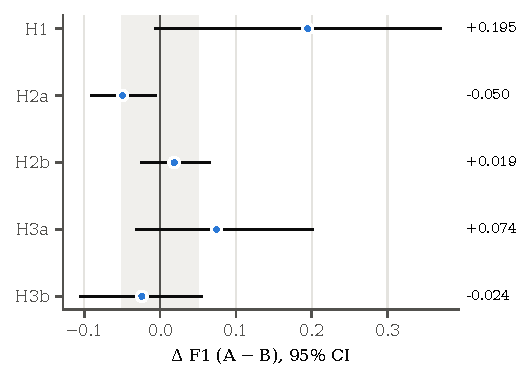
\includegraphics[width=\columnwidth]{figures/fig_confirmatory_D1.pdf}
\caption{Confirmatory F1 differences with 95\% CIs (D1-test, judge M1). Shaded band: the $\pm0.05$ equivalence margin.}\label{fig:forest}
\end{figure}

\begin{figure}[!htb]
\centering
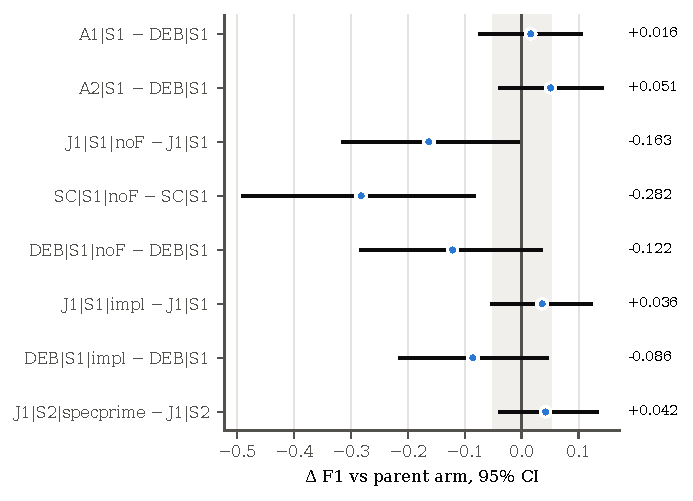
\includegraphics[width=\columnwidth]{figures/fig_e4_ablations_D1.pdf}
\caption{E4: F1 difference of each ablation from its parent arm with 95\% CIs (D1-test, judge M1). Shaded band: $\pm0.05$.}\label{fig:abl}
\end{figure}

\begin{figure*}[!htb]
\centering
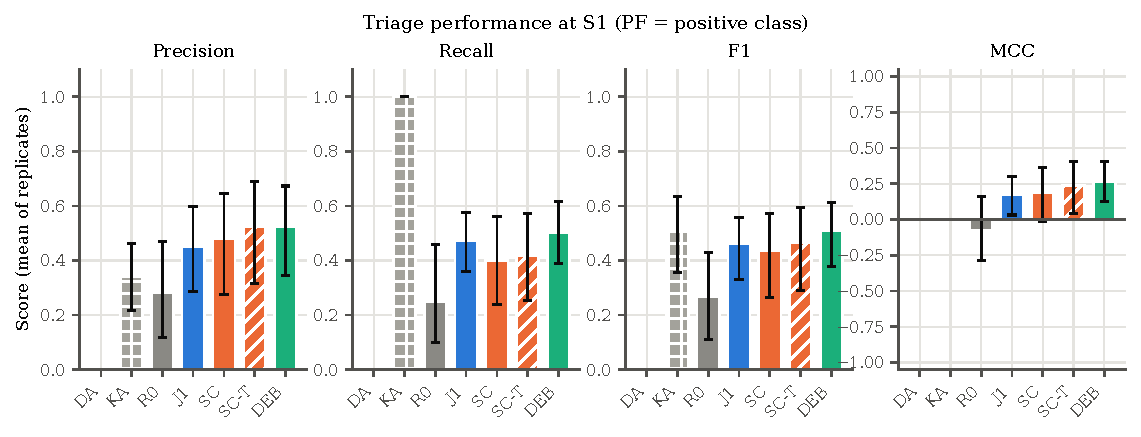
\includegraphics[width=\textwidth]{figures/fig_e1_prf_D1.pdf}
\caption{E1: precision, recall, F1 and MCC at S1 on D1-test (judge M1) with bug-level 95\% CIs. Hatched bars: keep-all (grid) and the token-matched SC-T arm.}\label{fig:prf}
\end{figure*}

\begin{table}[!htb]
\caption{E2: F1 (MCC) by specification level and arm, D1-test, judge M1, mean of \V{frozen:decoding:replicates} replicates. S0: signature; S1: + Javadoc; S2: + inferred specification.}\label{tab:e2}
\footnotesize\setlength{\tabcolsep}{3pt}
\begin{tabular}{@{}l c c c@{}}
\toprule
Level & J1 & SC & DEB \\
\midrule
S0 & \V{d1:J1|S0:f1} (\V{d1:J1|S0:mcc}) & \V{d1:SC|S0:f1} (\V{d1:SC|S0:mcc}) & \V{d1:DEB|S0:f1} (\V{d1:DEB|S0:mcc}) \\
S1 & \V{d1:J1|S1:f1} (\V{d1:J1|S1:mcc}) & \V{d1:SC|S1:f1} (\V{d1:SC|S1:mcc}) & \V{d1:DEB|S1:f1} (\V{d1:DEB|S1:mcc}) \\
S2 & \V{d1:J1|S2:f1} (\V{d1:J1|S2:mcc}) & \V{d1:SC|S2:f1} (\V{d1:SC|S2:mcc}) & \V{d1:DEB|S2:f1} (\V{d1:DEB|S2:mcc}) \\
\bottomrule
\end{tabular}
\end{table}


\begin{table*}[!htb]
\caption{Base papers. Reported results are taken from the original papers (*).}\label{tab:base}
\scriptsize\setlength{\tabcolsep}{3pt}
\begin{tabularx}{\textwidth}{@{}p{2.1cm} Y Y Y Y@{}}
\toprule
Paper (year) & Problem; method & Data; metric & Reported result (*) & Limitation for triage \\
\midrule
Xie et al., MACO (2026)~\cite{xie2026maco} & generation; cooperating agents with coverage feedback & \V{cit:maco methods} Java methods; line/branch coverage & \V{cit:maco line}\%, \V{cit:maco branch}\%\cited & current code only; budgets not aligned \\
Xu et al., CANDOR (2026)~\cite{xu2026candor} & generation and oracles; consensus panel & HumanEvalJava, LeetCodeJava; oracle correctness & \V{cit:candor lo}--\V{cit:candor hi}\cited & dependency-free methods \\
Liu et al., JSTestCraft (2026)~\cite{liu2026jstestcraft} & generation; context agents, three-LLM triage vote & \V{cit:jstestcraft repos} Node.js repositories; audited recall & triage recall \V{cit:jstestcraft recall}\%\cited & recall from one small audit \\
Gu et al., TestART (2026)~\cite{gu2026testart} & generation with template repair & Defects4J; pass rate & \V{cit:testart pass}\%\cited & rewrites assertions to observed values \\
Hayet et al., ChatAssert (2025)~\cite{hayet2025chatassert} & oracle generation with dynamic repair & TECO data; Acc@1 & +\V{cit:chatassert}\%\cited & match-based; presumes correct code \\
Taherkhani et al., VALTEST (2026)~\cite{taherkhani2026valtest} & test validity from semantic entropy & HumanEval, MBPP, LeetCode; validity & up to +\V{cit:valtest}\%\cited & validity from a reference solution \\
Walczak et al. (2026)~\cite{walczak2026context} & context levels for generation & \V{cit:walczak methods} custom methods; branch coverage & docstrings +\V{cit:walczak docstring} pp\cited & correct code only \\
Li et al., MitGen (2026)~\cite{li2026mitgen} & failing-test generation via reference implementations & EvoEval, ClassEval; failing-test recall & \V{cit:mitgen ours} vs \V{cit:mitgen base}\cited & single-statement faults \\
Yaraghi et al., TaRGET (2025)~\cite{yaraghi2025target} & test repair with fine-tuned code models & TaRBench; exact match & \V{cit:target em}\%\cited & assumes the test is wrong \\
Maddila et al. (2026)~\cite{maddila2026agentic} & agentic program repair after rule-based triage & Meta monorepo; solve rate & \V{cit:maddila solve}\%\cited & triage not evaluated \\
\bottomrule
\end{tabularx}
\end{table*}

\begin{table*}[!htb]
\caption{E5: F1 (MCC) at S1 by dataset and judge. Baselines do not depend on the judge. D2 F1 is not comparable with D1 F1 (different \PF{} prevalence).}\label{tab:robust}
\footnotesize
\begin{tabular}{@{}l c c c c@{}}
\toprule
 & \multicolumn{2}{c}{D1-test} & \multicolumn{2}{c}{D2 (seeded)} \\
\cmidrule(lr){2-3}\cmidrule(lr){4-5}
Arm & M1 (9B) & M2 (12B) & M1 (9B) & M2 (12B) \\
\midrule
\PF{} prevalence & \multicolumn{2}{c}{\V{sum:prevalence:pf_prevalence}} & \multicolumn{2}{c}{\V{sum2:prevalence:pf_prevalence}} \\
KA & \multicolumn{2}{c}{\V{d1:KA:f1} (\V{d1:KA:mcc})} & \multicolumn{2}{c}{\V{d2:KA:f1} (\V{d2:KA:mcc})} \\
R0 & \multicolumn{2}{c}{\V{d1:R0:f1} (\V{d1:R0:mcc})} & \multicolumn{2}{c}{\V{d2:R0:f1} (\V{d2:R0:mcc})} \\
J1 & \V{d1:J1|S1:f1} (\V{d1:J1|S1:mcc}) & \V{d1m2:J1|S1:f1} (\V{d1m2:J1|S1:mcc}) & \V{d2:J1|S1:f1} (\V{d2:J1|S1:mcc}) & \V{d2m2:J1|S1:f1} (\V{d2m2:J1|S1:mcc}) \\
SC & \V{d1:SC|S1:f1} (\V{d1:SC|S1:mcc}) & \V{d1m2:SC|S1:f1} (\V{d1m2:SC|S1:mcc}) & \V{d2:SC|S1:f1} (\V{d2:SC|S1:mcc}) & \V{d2m2:SC|S1:f1} (\V{d2m2:SC|S1:mcc}) \\
DEB & \V{d1:DEB|S1:f1} (\V{d1:DEB|S1:mcc}) & \V{d1m2:DEB|S1:f1} (\V{d1m2:DEB|S1:mcc}) & \V{d2:DEB|S1:f1} (\V{d2:DEB|S1:mcc}) & \V{d2m2:DEB|S1:f1} (\V{d2m2:DEB|S1:mcc}) \\
\bottomrule
\end{tabular}
\end{table*}


\begin{table*}[!htb]
\caption{How the arms here map to the base papers' approaches. All are re-implemented on this study's evidence package, labels and judge; none uses the original code.}\label{tab:reimpl}
\scriptsize\setlength{\tabcolsep}{2.5pt}
\begin{tabularx}{\textwidth}{@{}>{\raggedright\arraybackslash}p{1.45cm} >{\raggedright\arraybackslash}p{4.2cm} Y@{}}
\toprule
Arm & Original approach & Fidelity (matches / differs / why) \\
\midrule
DA & TestART~\cite{gu2026testart}, ChatAssert~\cite{hayet2025chatassert}, TaRGET~\cite{yaraghi2025target} & \emph{Matches} their premise that a failing test is wrong. \emph{Differs}: no repair step; DA is the limit case, since any repair of a program-fault test removes the bug evidence. \\
R0 & Maddila et al.~\cite{maddila2026agentic}; alarm triage~\cite{herzig2015alarms} & \emph{Matches} rule-based, model-free triage. \emph{Differs}: one rule on failure type and deepest project frame; no reproducibility checks or bisection. \\
DEB & JavaOracle debate~\cite{fu2026javaoracle} & \emph{Matches} adversarial agents and an adjudicator. \emph{Differs}: fixed five-call budget, anonymised random argument order, cited evidence, local 9B judge. \\
SC & JSTestCraft vote~\cite{liu2026jstestcraft}; self-consistency~\cite{wang2023selfconsistency} & \emph{Matches} majority voting. \emph{Differs}: five samples of one model, not three models. \\
VOTE3/5 & JSTestCraft three-LLM vote~\cite{liu2026jstestcraft} & \emph{Matches} a three-family majority. \emph{Differs}: local, budget-matched. E8: F1 \V{e8:summary:VOTE3|S1:f1} vs SC3 \V{e8:summary:SC3|S1:f1}, $\Delta$ \V{e8:hypotheses:H8-1:delta} \V{e8:hypotheses:H8-1:ci95}, $p_\mathrm{Holm}$ \V{e8:hypotheses:H8-1:p_holm}. \\
Zhao et al.\ finding & effective generated tests: \V{cit:zhao lo}--\V{cit:zhao hi}\%\cited{} over six models~\cite{zhao2026misguidance} & \emph{Not replicated} (rule fixed in advance): \V{zhao:subsets:all_D1:share_effective_pct@2}\% \V{zhao:subsets:all_D1:ci95_pct@ci2} effective; the interval overlaps their range, and the qualitative finding (about \V{zhao:subsets:all_D1:share_effective_pct@0}\% of generated tests reveal the bug) holds. \emph{Differs}: one generator vs their six, reconstructed frame, Defects4J~3.0.1. \\
\bottomrule
\end{tabularx}
\end{table*}

\begin{figure*}[t]
\centering
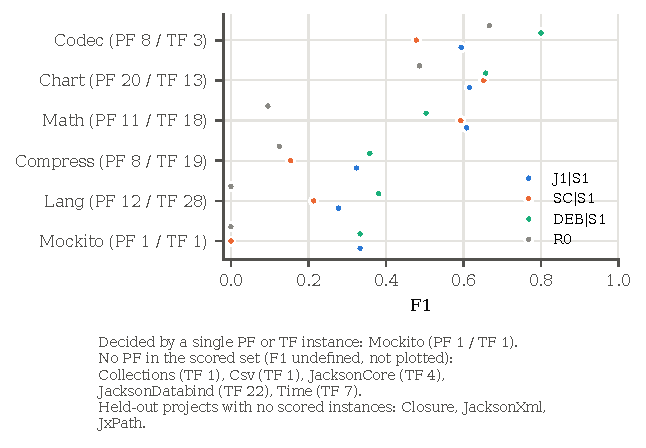
\includegraphics[width=0.8\textwidth]{figures/fig_r5_per_project_D1.pdf}
\caption{Per-project F1 at S1 on D1-test (judge M1), projects with both classes.}\label{fig:perproject}
\end{figure*}

% D-81: not a float, so it stays directly below the Appendix B heading (same numbering and caption style)
\par\medskip\noindent\begin{minipage}{\columnwidth}{\footnotesize\refstepcounter{table}\label{tab:sens}\textbf{Table~\thetable}\enspace Sensitivity of F1 (MCC) at S1, D1-test, judge M1: invalid outputs excluded instead of scored \TF; AMB counted as \PF{} or as \TF.\par}\smallskip
{\noindent \footnotesize
\begin{tabular}{@{}l c c c@{}}
\toprule
Arm & invalid excluded & AMB as \PF & AMB as \TF \\
\midrule
R0 & \V{sum:sensitivity_f1:invalid_excluded:R0:f1} (\V{sum:sensitivity_f1:invalid_excluded:R0:mcc}) & \V{sum:sensitivity_f1:AMB_as_PF:R0:f1} (\V{sum:sensitivity_f1:AMB_as_PF:R0:mcc}) & \V{sum:sensitivity_f1:AMB_as_TF:R0:f1} (\V{sum:sensitivity_f1:AMB_as_TF:R0:mcc}) \\
J1 & \V{sum:sensitivity_f1:invalid_excluded:J1|S1:f1} (\V{sum:sensitivity_f1:invalid_excluded:J1|S1:mcc}) & \V{sum:sensitivity_f1:AMB_as_PF:J1|S1:f1} (\V{sum:sensitivity_f1:AMB_as_PF:J1|S1:mcc}) & \V{sum:sensitivity_f1:AMB_as_TF:J1|S1:f1} (\V{sum:sensitivity_f1:AMB_as_TF:J1|S1:mcc}) \\
SC & \V{sum:sensitivity_f1:invalid_excluded:SC|S1:f1} (\V{sum:sensitivity_f1:invalid_excluded:SC|S1:mcc}) & \V{sum:sensitivity_f1:AMB_as_PF:SC|S1:f1} (\V{sum:sensitivity_f1:AMB_as_PF:SC|S1:mcc}) & \V{sum:sensitivity_f1:AMB_as_TF:SC|S1:f1} (\V{sum:sensitivity_f1:AMB_as_TF:SC|S1:mcc}) \\
DEB & \V{sum:sensitivity_f1:invalid_excluded:DEB|S1:f1} (\V{sum:sensitivity_f1:invalid_excluded:DEB|S1:mcc}) & \V{sum:sensitivity_f1:AMB_as_PF:DEB|S1:f1} (\V{sum:sensitivity_f1:AMB_as_PF:DEB|S1:mcc}) & \V{sum:sensitivity_f1:AMB_as_TF:DEB|S1:f1} (\V{sum:sensitivity_f1:AMB_as_TF:DEB|S1:mcc}) \\
\bottomrule
\end{tabular}
\par}\end{minipage}\par\medskip



% D-81: not a float, so it stays directly below the Appendix B heading (same numbering and caption style)
\par\medskip\noindent\begin{minipage}{\columnwidth}{\footnotesize\refstepcounter{table}\label{tab:cost}\textbf{Table~\thetable}\enspace Cost and latency per arm from the call logs, D1-test, S1, judge M1, \V{cost:scored_instances} scored instances $\times$ \V{cost:arms:DEB:replicates} replicates. Tokens: mean per instance; wall time per instance (calls run one at a time). API cost: zero.\par}\smallskip
{\noindent \footnotesize\setlength{\tabcolsep}{3.5pt}
\begin{tabular}{@{}l c c c c c@{}}
\toprule
Arm & Calls & In tokens & Out tokens & Median (s) & P90 (s) \\
\midrule
J1 & \V{cost:arms:J1:calls_per_instance@0} & \V{cost:arms:J1:input_tokens_per_instance@0} & \V{cost:arms:J1:output_tokens_per_instance@0} & \V{cost:arms:J1:wall_s_median@2} & \V{cost:arms:J1:wall_s_p90@2} \\
SC & \V{cost:arms:SC:calls_per_instance@0} & \V{cost:arms:SC:input_tokens_per_instance@0} & \V{cost:arms:SC:output_tokens_per_instance@0} & \V{cost:arms:SC:wall_s_median@2} & \V{cost:arms:SC:wall_s_p90@2} \\
SC-T & \V{cost:arms:SC-T:calls_per_instance@0} & \V{cost:arms:SC-T:input_tokens_per_instance@0} & \V{cost:arms:SC-T:output_tokens_per_instance@0} & \V{cost:arms:SC-T:wall_s_median@2} & \V{cost:arms:SC-T:wall_s_p90@2} \\
DEB & \V{cost:arms:DEB:calls_per_instance@0} & \V{cost:arms:DEB:input_tokens_per_instance@0} & \V{cost:arms:DEB:output_tokens_per_instance@0} & \V{cost:arms:DEB:wall_s_median@2} & \V{cost:arms:DEB:wall_s_p90@2} \\
\bottomrule
\end{tabular}
\par}\end{minipage}\par\medskip


\paragraph{Failure cases.} Per-project F1 (Appendix~\ref{app:extra}) is lowest on Compress and Lang for DEB (\V{sum:per_project_f1:DEB|S1:Compress} and \V{sum:per_project_f1:DEB|S1:Lang}); a project whose sample holds only test faults, such as JacksonDatabind (\V{sum:per_project_counts:JacksonDatabind:TF} \TF, \V{sum:per_project_counts:JacksonDatabind:PF} \PF), can contribute only false alarms. Of the three program faults in Table~\ref{tab:qual}, \QcaseA{} turns on the expected and actual values in the failure message (cf.\ A4), in \QcaseB{} the judge takes documented buggy behaviour as the contract (cf.\ H2a, A5a), and in \QcaseC{} it inverts the failure evidence, a limit of the small judge.

\section{Post hoc and exploratory analyses}\label{app:explore}
\setcounter{table}{0}\setcounter{figure}{0}% numbering restarts in each appendix
All analyses here are post hoc (D-80) or exploratory (D-82): their rules were fixed before they were computed, none is a confirmatory test, and none is corrected for multiplicity.

\paragraph{Specification mixed model.} An exploratory mixed model on \PF{} recall, with bug-level cluster-bootstrap intervals (\V{glmmb:B} refits), estimates odds ratios of \V{glmmb:models:PF_recall:terms:1:odds_ratio} \V{glmmb:models:PF_recall:terms:1:or_ci95_bootstrap} for S0 and \V{glmmb:models:PF_recall:terms:2:odds_ratio} \V{glmmb:models:PF_recall:terms:2:or_ci95_bootstrap} for S2 relative to S1; on \TF{} instances the S0 odds ratio is \V{glmmb:models:TF_specificity:terms:1:odds_ratio} \V{glmmb:models:TF_specificity:terms:1:or_ci95_bootstrap}. All three intervals include 1, so the model adds no evidence of a specification effect beyond the contrasts above. Its variational intervals under-covered in simulation, so it is reported only with bootstrap intervals; a population-averaged GEE with bugs as clusters and bias-reduced sandwich errors (sensitivity, D-120) gives \PF{}-recall odds ratios of \V{rv19:mixed_model:gee:PF_recall:terms:1:odds_ratio} \V{rv19:mixed_model:gee:PF_recall:terms:1:or_ci95_robust} for S0 and \V{rv19:mixed_model:gee:PF_recall:terms:2:odds_ratio} \V{rv19:mixed_model:gee:PF_recall:terms:2:or_ci95_robust} for S2, again including 1.

\paragraph{Summary.} The practical takeaway is the cost-ratio break-even: DEB beats keeping every failure only while a missed bug costs less than \V{xd:D1:DEB:breakeven_vs_KA@2} false alarms (\V{xd:D1:DEB:breakeven_vs_KA_natural@2} at the natural prevalence). The practical selective rule is DEB's at $\tau=\V{sel:arms:DEB:tau}$ (tuned on dev): it discards \V{sel:arms:DEB:share_discarded@pct} of failures, loses \V{sel:arms:DEB:pf_lost@1} of \V{sel:arms:DEB:pf_in_set} bugs per replicate and gains \V{sel:arms:DEB:delta_f1_vs_ka} F1 over keep-all (\V{sel:arms:DEB:delta_f1_vs_ka_ci95}); SC's rule at $\tau=\V{sel:arms:SC:tau}$ discards more but loses \V{sel:arms:SC:pf_lost@0} of \V{sel:arms:SC:pf_in_set} bugs (Table~\ref{tab:selka}). SC's rule did not transfer to the third-family judge (H6-3 \V{e6b:hypotheses:H6-3:delta}, not supported), and DEB's has been evaluated on M1 only. The judges are overconfident (DEB: stated confidence \V{xd:D2:calibration:DEB:mean_confidence@2}, accuracy \V{xd:D2:calibration:DEB:accuracy@2}), and escalating split SC votes to DEB did not beat DEB alone.

\paragraph{Development gate versus held-out result.} M1's one-shot F1 was far below R0's on the development pilot (\V{devgate:G_d_detail:J1_f1} vs \V{devgate:G_d_detail:R0_f1}; \V{devgate:n_instances} instances) and above it on the held-out split (\V{d1:J1|S1:f1} vs \V{d1:R0:f1}); with \V{devgate:n_bugs} bugs the pilot's interval, \V{devgate:G_d_detail:delta_ci95_bug_bootstrap}, spanned both, so the gate measured project composition more than judge quality.

\par\medskip\noindent\begin{minipage}{\columnwidth}{\footnotesize\refstepcounter{table}\label{tab:mde}\textbf{Table~\thetable}\enspace Post hoc sensitivity analysis (not observed power): minimum detectable $\Delta$F1 at \V{mde:power@pct0} power, $\mathrm{MDE}=(z_{1-\alpha/2}+z_{\V{mde:power@1}})\,\mathrm{SE}$, SE: standard deviation of the bug-level bootstrap $\Delta$F1, at $\alpha=\V{mde:alpha@2}$ and at the Holm $\alpha$ for the smallest $p$ (\V{mde:alpha_holm_smallest_p@2}).\par}\smallskip
{\noindent \footnotesize\setlength{\tabcolsep}{3.5pt}
\begin{tabular}{@{}l c c c c c@{}}
\toprule
H & $n$ (bugs) & $\Delta$F1 & SE & MDE$_{\V{mde:alpha@2}}$ & MDE$_{\V{mde:alpha_holm_smallest_p@2}}$ \\
\midrule
H1 & \V{mde:tests:H1:n_instances} (\V{mde:tests:H1:n_bugs}) & \V{mde:tests:H1:delta} & \V{mde:tests:H1:se_bootstrap} & \V{mde:tests:H1:mde_alpha_005} & \V{mde:tests:H1:mde_alpha_holm_min} \\
H2a & \V{mde:tests:H2a:n_instances} (\V{mde:tests:H2a:n_bugs}) & \V{mde:tests:H2a:delta} & \V{mde:tests:H2a:se_bootstrap} & \V{mde:tests:H2a:mde_alpha_005} & \V{mde:tests:H2a:mde_alpha_holm_min} \\
H2b & \V{mde:tests:H2b:n_instances} (\V{mde:tests:H2b:n_bugs}) & \V{mde:tests:H2b:delta} & \V{mde:tests:H2b:se_bootstrap} & \V{mde:tests:H2b:mde_alpha_005} & \V{mde:tests:H2b:mde_alpha_holm_min} \\
H3a & \V{mde:tests:H3a:n_instances} (\V{mde:tests:H3a:n_bugs}) & \V{mde:tests:H3a:delta} & \V{mde:tests:H3a:se_bootstrap} & \V{mde:tests:H3a:mde_alpha_005} & \V{mde:tests:H3a:mde_alpha_holm_min} \\
H3b & \V{mde:tests:H3b:n_instances} (\V{mde:tests:H3b:n_bugs}) & \V{mde:tests:H3b:delta} & \V{mde:tests:H3b:se_bootstrap} & \V{mde:tests:H3b:mde_alpha_005} & \V{mde:tests:H3b:mde_alpha_holm_min} \\
\bottomrule
\end{tabular}
\par}\end{minipage}\par\medskip
\par\medskip\noindent\begin{minipage}{\columnwidth}{\footnotesize\refstepcounter{figure}\label{fig:spec}\textbf{Fig.~\thefigure}\enspace E2: F1 by specification level for J1, SC and DEB on D1-test (judge M1), bug-level 95\% CIs.\par}\smallskip
{\noindent\centering 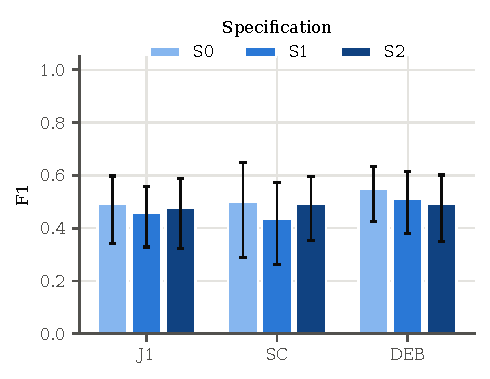
\includegraphics[width=0.8\columnwidth]{figures/fig_e2_spec_f1_D1.pdf}
\par}\end{minipage}\par\medskip
\par\medskip\noindent\begin{minipage}{\columnwidth}{\footnotesize\refstepcounter{figure}\label{fig:pareto}\textbf{Fig.~\thefigure}\enspace E3: F1 against consumed tokens per instance at S1 (D1-test, judge M1), bug-level 95\% CIs.\par}\smallskip
{\noindent\centering 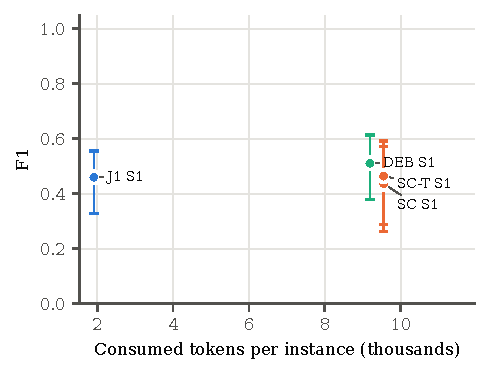
\includegraphics[width=0.85\columnwidth]{figures/fig_e3_pareto_D1.pdf}
\par}\end{minipage}\par\medskip
\par\medskip\noindent\begin{minipage}{\columnwidth}{\footnotesize\refstepcounter{table}\label{tab:explore}\textbf{Table~\thetable}\enspace Exploratory analyses (D-82), D1-test, S1, judge M1. $r$: cost of a missed bug in false alarms. $\tau$: confidence threshold tuned on the development pilot only. Bug-level 95\% CIs; no correction.\par}\smallskip
{\noindent\scriptsize\setlength{\tabcolsep}{2.5pt}
\begin{tabularx}{\columnwidth}{@{}Y >{\raggedright\arraybackslash}p{3.45cm}@{}}
\toprule
Quantity & Value \\
\midrule
Cost ratio: DEB cheaper than KA iff $r<$ & \V{xd:D1:DEB:breakeven_vs_KA@2} (natural \V{xd:D1:DEB:breakeven_vs_KA_natural@2}) \\
Cost ratio: DEB cheaper than DA iff $r>$ & \V{xd:D1:DEB:breakeven_vs_DA@2} (natural \V{xd:D1:DEB:breakeven_vs_DA_natural@2}) \\
Cost ratio: J1 / SC cheaper than KA iff $r<$ & \V{xd:D1:J1:breakeven_vs_KA@2} / \V{xd:D1:SC:breakeven_vs_KA@2} \\
ECE: J1 / SC / DEB & \V{xd:D2:calibration:J1:ece} / \V{xd:D2:calibration:SC:ece} / \V{xd:D2:calibration:DEB:ece} \\
DEB mean confidence vs accuracy & \V{xd:D2:calibration:DEB:mean_confidence} vs \V{xd:D2:calibration:DEB:accuracy} \\
Selective SC ($\tau$=\V{xd:D2:selective:SC:tau}): F1, $\Delta$F1 & \V{xd:D2:selective:SC:f1}, \V{xd:D2:selective:SC:delta_f1} \V{xd:D2:selective:SC:delta_f1_ci95} \\
Selective J1 ($\tau$=\V{xd:D2:selective:J1:tau}): F1, $\Delta$F1 & \V{xd:D2:selective:J1:f1}, \V{xd:D2:selective:J1:delta_f1} \V{xd:D2:selective:J1:delta_f1_ci95} \\
Selective DEB ($\tau$=\V{xd:D2:selective:DEB:tau}): F1, $\Delta$F1 & \V{xd:D2:selective:DEB:f1}, \V{xd:D2:selective:DEB:delta_f1} \V{xd:D2:selective:DEB:delta_f1_ci95} \\
SC$\to$DEB cascade: escalated / F1 & \V{xd:D3:escalation_rate@pct} / \V{xd:D3:f1} \\
Cascade $-$ SC; $-$ DEB ($\Delta$F1) & \V{xd:D3:vs_SC:delta} \V{xd:D3:vs_SC:ci95}; \V{xd:D3:vs_DEB:delta} \V{xd:D3:vs_DEB:ci95} \\
Cascade tokens (SC / DEB) & \V{xd:D3:tokens_per_instance@0} (\V{xd:D3:sc_tokens_per_instance@0} / \V{xd:D3:deb_tokens_per_instance@0}) \\
Concession rate, round 1 / 2 & \V{xd:D4:concession_rate_r1@pct} / \V{xd:D4:concession_rate_r2@pct} \\
Sided with last-presented ($p$ vs 0.5) & \V{xd:D4:last_presented_share@pct} (\V{xd:D4:last_presented_p}) \\
DEB differs from SC majority; DEB right then & \V{xd:D4:flip_rate_vs_sc_majority@pct}; \V{xd:D4:deb_correct_share_among_flips@pct} \\
\bottomrule
\end{tabularx}
\par}\end{minipage}\par\medskip
\par\medskip\noindent\begin{minipage}{\columnwidth}{\footnotesize\refstepcounter{table}\label{tab:selka}\textbf{Table~\thetable}\enspace Selective triage against keep-all (exploratory, D-82), D1-test, S1, judge M1: discard only a TF stated with confidence $\geq\tau$ ($\tau$ tuned on the development pilot). Lost: PF tests discarded per replicate, of the PF instances in the set. The arm's own MCC is shown on its own (keep-all's MCC is 0).\par}\smallskip
{\noindent\scriptsize\setlength{\tabcolsep}{2.5pt}
\resizebox{\columnwidth}{!}{\begin{tabular}{@{}l c c c c c@{}}
\toprule
Arm & $\tau$ & $\Delta$F1 vs KA [95\% CI] & Lost & Discarded & MCC [95\% CI] \\
\midrule
DEB & \V{sel:arms:DEB:tau} & \V{sel:arms:DEB:delta_f1_vs_ka} \V{sel:arms:DEB:delta_f1_vs_ka_ci95} & \V{sel:arms:DEB:pf_lost@1} / \V{sel:arms:DEB:pf_in_set} & \V{sel:arms:DEB:share_discarded@pct} & \V{sel:arms:DEB:mcc} \V{sel:arms:DEB:mcc_ci95} \\
J1 & \V{sel:arms:J1:tau} & \V{sel:arms:J1:delta_f1_vs_ka} \V{sel:arms:J1:delta_f1_vs_ka_ci95} & \V{sel:arms:J1:pf_lost@1} / \V{sel:arms:J1:pf_in_set} & \V{sel:arms:J1:share_discarded@pct} & \V{sel:arms:J1:mcc} \V{sel:arms:J1:mcc_ci95} \\
SC & \V{sel:arms:SC:tau} & \V{sel:arms:SC:delta_f1_vs_ka} \V{sel:arms:SC:delta_f1_vs_ka_ci95} & \V{sel:arms:SC:pf_lost@1} / \V{sel:arms:SC:pf_in_set} & \V{sel:arms:SC:share_discarded@pct} & \V{sel:arms:SC:mcc} \V{sel:arms:SC:mcc_ci95} \\
\bottomrule
\end{tabular}}
\par}\end{minipage}\par\medskip

\section{Further judges, the vote and a frontier reference (E6, E8, E9)}\label{app:post}
\setcounter{table}{0}\setcounter{figure}{0}% numbering restarts in each appendix

\noindent\textit{Second judge (M2), detail.} On the same instances, M2 (12B) improved on M1 in every arm and dataset: on D1-test by \V{r3:D1:m2_minus_m1:J1:f1:delta} (J1), \V{r3:D1:m2_minus_m1:SC:f1:delta} (SC) and \V{r3:D1:m2_minus_m1:DEB:f1:delta} (DEB, 95\% CI \V{r3:D1:m2_minus_m1:DEB:f1:ci95}), and on D2 by \V{r3:D2:m2_minus_m1:J1:f1:delta}, \V{r3:D2:m2_minus_m1:SC:f1:delta} and \V{r3:D2:m2_minus_m1:DEB:f1:delta}. DEB ranks first by F1 and MCC under M2 on both datasets. M2's samples were almost unanimous, so its SC reproduced J1's F1 on D1-test. M2 shares the generator's family, so self-preference cannot be excluded.

Run after the primary results under rules fixed before any call (D-82, D-83; builds D-85, D-88, D-90): D1-test, S1, frozen prompts and decoding, one replicate, bug-level 95\% CIs. E6b and E8 test hypotheses fixed in advance with Holm within each family; E6a is exploratory. The E6b judge (Ministral~3 14B, neither Qwen nor Gemma) was the first of four candidates fixed in advance to pass Step~1 and gates G-a/G-b on the development pilot. VOTE3 is a majority of one fresh J1 call each from M1, M2 and E6b; VOTE5 of 2+2+1 further calls; SC3 is the majority of the first three of M1's committed SC samples.

\par\medskip\noindent\begin{minipage}{\columnwidth}{\footnotesize\refstepcounter{table}\label{tab:post}\textbf{Table~\thetable}\enspace E6b, E6a and E8 on D1-test, S1 (\V{e6b:n_instances} instances, \V{e6b:n_bugs} bugs); one replicate (M1: three). $\Delta$: paired difference, bug-level 95\% CI; $p_\mathrm{H}$: Holm within E6b or E8; H6-3 at the frozen $\tau=\V{e6b:hypotheses:H6-3:tau}$.\par}\smallskip
{\noindent\scriptsize\setlength{\tabcolsep}{4pt}
\resizebox{\columnwidth}{!}{\begin{tabular}{@{}l l r@{}}
\toprule
Quantity & Estimate [95\% CI] & $p_\mathrm{H}$ \\
\midrule
E6b F1: J1 / SC / DEB & \V{e6b:summary:J1:f1} / \V{e6b:summary:SC:f1} / \V{e6b:summary:DEB:f1} &  \\
E6b MCC: J1 / SC / DEB & \V{e6b:summary:J1:mcc} / \V{e6b:summary:SC:mcc} / \V{e6b:summary:DEB:mcc} &  \\
H6-1 $\Delta$F1 DEB$-$SC & \V{e6b:hypotheses:H6-1:delta} \V{e6b:hypotheses:H6-1:ci95} & \V{e6b:hypotheses:H6-1:p_holm} \\
H6-2 MCC(DEB) & \V{e6b:hypotheses:H6-2:mcc} \V{e6b:hypotheses:H6-2:ci95} & \V{e6b:hypotheses:H6-2:p_holm} \\
H6-3 selective SC$-$SC & \V{e6b:hypotheses:H6-3:delta} \V{e6b:hypotheses:H6-3:ci95} & -- \\
DEB $\Delta$F1 E6b$-$M2 & \V{e6b:family_check:e6b_minus:DEB E6B-M2:f1:delta} \V{e6b:family_check:e6b_minus:DEB E6B-M2:f1:ci95} &  \\
DEB $\Delta$F1 E6b$-$M1 & \V{e6b:family_check:e6b_minus:DEB E6B-M1:f1:delta} \V{e6b:family_check:e6b_minus:DEB E6B-M1:f1:ci95} &  \\
E6a 35B F1: J1 / DEB & \V{e6a:summary:35B:J1:f1} / \V{e6a:summary:35B:DEB:f1} &  \\
E6a DEB $\Delta$F1 35B$-$M1 & \V{e6a:35b_minus:DEB 35B-M1:f1:delta} \V{e6a:35b_minus:DEB 35B-M1:f1:ci95} &  \\
E8 F1: VOTE3 / VOTE5 & \V{e8:summary:VOTE3|S1:f1} / \V{e8:summary:VOTE5|S1:f1} &  \\
E8 MCC: VOTE3 / VOTE5 & \V{e8:summary:VOTE3|S1:mcc} / \V{e8:summary:VOTE5|S1:mcc} &  \\
M1 F1: SC3 / SC / DEB & \V{e8:summary:SC3|S1:f1} / \V{e8:summary:SC|S1:f1} / \V{e8:summary:DEB|S1:f1} &  \\
H8-1 VOTE3$-$SC3 & \V{e8:hypotheses:H8-1:delta} \V{e8:hypotheses:H8-1:ci95} & \V{e8:hypotheses:H8-1:p_holm} \\
H8-2 VOTE5$-$SC & \V{e8:hypotheses:H8-2:delta} \V{e8:hypotheses:H8-2:ci95} & \V{e8:hypotheses:H8-2:p_holm} \\
H8-3 VOTE5$-$DEB & \V{e8:hypotheses:H8-3:delta} \V{e8:hypotheses:H8-3:ci95} & \V{e8:hypotheses:H8-3:p_holm} \\
PF lost: VOTE3 / 5, SC, DEB & \V{e8:summary:VOTE3|S1:pf_lost@0} / \V{e8:summary:VOTE5|S1:pf_lost@0}, \V{e8:summary:SC|S1:pf_lost@0}, \V{e8:summary:DEB|S1:pf_lost@0} of \V{e6b:pf_prevalence:PF} &  \\
\bottomrule
\end{tabular}}
\par}\end{minipage}\par\medskip


\par\medskip\noindent\begin{minipage}{\columnwidth}{\footnotesize\refstepcounter{table}\label{tab:noise}\textbf{Table~\thetable}\enspace Replicate noise (exploratory, D-94): M1's three replicates scored separately at S1 on the \V{rn:n_instances} D1-test instances, against the single-replicate cross-model differences. A difference is \emph{beyond} M1's spread when $|\Delta|$ exceeds the range of M1's replicates for the arm compared. No test.\par}\smallskip
{\noindent\scriptsize\setlength{\tabcolsep}{4pt}
\resizebox{\columnwidth}{!}{\begin{tabular}{@{}l l c c c@{}}
\toprule
M1 arm & F1 per replicate & F1 range & F1 SD & MCC range \\
\midrule
J1 & \V{rn:noise:J1:f1:per_replicate:0} / \V{rn:noise:J1:f1:per_replicate:1} / \V{rn:noise:J1:f1:per_replicate:2} & \V{rn:noise:J1:f1:range} & \V{rn:noise:J1:f1:sd} & \V{rn:noise:J1:mcc:range} \\
SC & \V{rn:noise:SC:f1:per_replicate:0} / \V{rn:noise:SC:f1:per_replicate:1} / \V{rn:noise:SC:f1:per_replicate:2} & \V{rn:noise:SC:f1:range} & \V{rn:noise:SC:f1:sd} & \V{rn:noise:SC:mcc:range} \\
SC-T & \V{rn:noise:SC-T:f1:per_replicate:0} / \V{rn:noise:SC-T:f1:per_replicate:1} / \V{rn:noise:SC-T:f1:per_replicate:2} & \V{rn:noise:SC-T:f1:range} & \V{rn:noise:SC-T:f1:sd} & \V{rn:noise:SC-T:mcc:range} \\
DEB & \V{rn:noise:DEB:f1:per_replicate:0} / \V{rn:noise:DEB:f1:per_replicate:1} / \V{rn:noise:DEB:f1:per_replicate:2} & \V{rn:noise:DEB:f1:range} & \V{rn:noise:DEB:f1:sd} & \V{rn:noise:DEB:mcc:range} \\
SC3 & \V{rn:noise:SC3:f1:per_replicate:0} / \V{rn:noise:SC3:f1:per_replicate:1} / \V{rn:noise:SC3:f1:per_replicate:2} & \V{rn:noise:SC3:f1:range} & \V{rn:noise:SC3:f1:sd} & \V{rn:noise:SC3:mcc:range} \\
\midrule
Difference (F1) & $\Delta$ & M1 range & & \\
\midrule
J1: M2$-$M1 & \V{rn:cross_model:0:delta} & \V{rn:cross_model:0:m1_range} & beyond & \\
SC: M2$-$M1 & \V{rn:cross_model:2:delta} & \V{rn:cross_model:2:m1_range} & beyond & \\
DEB: M2$-$M1 & \V{rn:cross_model:4:delta} & \V{rn:cross_model:4:m1_range} & within & \\
J1: E6b$-$M1 & \V{rn:cross_model:1:delta} & \V{rn:cross_model:1:m1_range} & beyond & \\
SC: E6b$-$M1 & \V{rn:cross_model:3:delta} & \V{rn:cross_model:3:m1_range} & beyond & \\
DEB: E6b$-$M1 & \V{rn:cross_model:5:delta} & \V{rn:cross_model:5:m1_range} & within & \\
J1: 35B$-$M1 & \V{rn:cross_model:6:delta} & \V{rn:cross_model:6:m1_range} & beyond & \\
DEB: 35B$-$M1 & \V{rn:cross_model:7:delta} & \V{rn:cross_model:7:m1_range} & within & \\
VOTE3$-$SC3 & \V{rn:cross_model:8:delta} & \V{rn:cross_model:8:m1_range} & beyond & \\
VOTE5$-$SC & \V{rn:cross_model:9:delta} & \V{rn:cross_model:9:m1_range} & beyond & \\
VOTE5$-$DEB & \V{rn:cross_model:10:delta} & \V{rn:cross_model:10:m1_range} & within & \\
\bottomrule
\end{tabular}}
\par}\end{minipage}\par\medskip


\par\medskip\noindent\begin{minipage}{\columnwidth}{\footnotesize\refstepcounter{table}\label{tab:gap}\textbf{Table~\thetable}\enspace Why our numbers differ from the base papers, and where they agree. * taken from the paper.\par}\smallskip
{\noindent\scriptsize\setlength{\tabcolsep}{2.5pt}
\begin{tabularx}{\columnwidth}{@{}>{\raggedright\arraybackslash}p{1.35cm} Y Y@{}}
\toprule
Paper & Differs from ours in & Agrees with ours on \\
\midrule
Zhao et al.~\cite{zhao2026misguidance} & six API generators vs one local; Defects4J~3.0 vs 3.0.1; reconstructed frame & effective-test share: \V{zhao:subsets:all_D1:share_effective_pct@2}\% \V{zhao:subsets:all_D1:ci95_pct@ci2} overlaps \V{cit:zhao lo}--\V{cit:zhao hi}\%\cited \\
JSTestCraft~\cite{liu2026jstestcraft} & JavaScript; recall from a small manual audit; API models; three-model vote inside generation & a cross-family vote keeps recall high: \V{e8:summary:VOTE3|S1:recall} vs \V{cit:jstestcraft recall}\%\cited \\
JavaOracle~\cite{fu2026javaoracle} & oracle generation, not triage; precision on its own labels; API models; debate ablated, not budget-matched & debate trades away true positives: DEB discards \V{d1:DEB|S1:pf_lost@0} of \V{sum:prevalence:PF}; theirs fall \V{cit:javaoracle tp before} to \V{cit:javaoracle tp after}\cited \\
MACO, TestART, CANDOR~\cite{xie2026maco,gu2026testart,xu2026candor} & generation metrics (coverage, pass rate, oracle correctness) on the current version; no prevalence of faults & none directly: no triage result \\
\bottomrule
\end{tabularx}
\par}\end{minipage}\par\medskip


\par\medskip\noindent\begin{minipage}{\columnwidth}{\footnotesize\refstepcounter{table}\label{tab:e9}\textbf{Table~\thetable}\enspace E9, frontier reference point, not a protocol replication (D-92, D-97): Claude Sonnet~5.5 through the Message Batches API on the \V{e9:n_instances} scored D1-test instances; J1 one replicate, DEB three; default sampling, no seeds, thinking off; spend US\$\,\V{e9:spend_usd@2}.\par}\smallskip
{\noindent\scriptsize\setlength{\tabcolsep}{4pt}
\resizebox{\columnwidth}{!}{\begin{tabular}{@{}l l r@{}}
\toprule
Quantity & Estimate [95\% CI] & $p_\mathrm{H}$ \\
\midrule
Sonnet F1: J1 / DEB & \V{e9:summary:J1|S1|SON:f1} / \V{e9:summary:DEB|S1|SON:f1} & \\
Sonnet MCC: J1 / DEB & \V{e9:summary:J1|S1|SON:mcc} / \V{e9:summary:DEB|S1|SON:mcc} & \\
H9-1 $\Delta$F1 DEB$-$J1 & \V{e9:hypotheses:H9-1:delta} \V{e9:hypotheses:H9-1:ci95} & \V{e9:hypotheses:H9-1:p_holm} \\
H9-2 MCC(DEB) & \V{e9:hypotheses:H9-2:mcc} \V{e9:hypotheses:H9-2:ci95} & \V{e9:hypotheses:H9-2:p_holm} \\
DEB $\Delta$F1 Sonnet$-$M1 & \V{e9:sonnet_minus_m1:DEB:f1:delta} \V{e9:sonnet_minus_m1:DEB:f1:ci95} & \\
J1 $\Delta$F1 Sonnet$-$M1 & \V{e9:sonnet_minus_m1:J1:f1:delta} \V{e9:sonnet_minus_m1:J1:f1:ci95} & \\
DEB F1 per replicate: Sonnet & \V{e9:deb_run_to_run_spread:sonnet:f1:per_replicate:0} / \V{e9:deb_run_to_run_spread:sonnet:f1:per_replicate:1} / \V{e9:deb_run_to_run_spread:sonnet:f1:per_replicate:2} & \\
DEB F1 per replicate: M1 & \V{e9:deb_run_to_run_spread:m1:f1:per_replicate:0} / \V{e9:deb_run_to_run_spread:m1:f1:per_replicate:1} / \V{e9:deb_run_to_run_spread:m1:f1:per_replicate:2} & \\
PF lost: Sonnet J1 / DEB; M1 DEB & \V{e9:summary:J1|S1|SON:pf_lost@0} / \V{e9:summary:DEB|S1|SON:pf_lost@1}; \V{e9:summary:DEB|S1:pf_lost@0} & \\
\bottomrule
\end{tabular}}
\par}\end{minipage}\par\medskip

\noindent\textit{Reading.} The third-family judge confirms that DEB is above chance (H6-2) but not that it beats SC (H6-1); the selective rule did not transfer (H6-3). M2, which shares the generator's family, scored above E6b in every arm, consistent with family affinity but confounded with model and size. The vote's gains over SC3 and SC were not significant after Holm, but it lost far fewer bug-revealing tests. The frontier judge is a reference point, not a replication: it shows how much of the gap to the base papers a larger model closes, and its three DEB replicates vary far less than M1's. Its training data very likely include Defects4J and its fixes, so its D1 score may be inflated by memorisation; E9b (D-104) judged the D2 seeded faults, whose fixes no model can have seen, and found no drop (Appendix~\ref{app:cascade}). \textit{Disclosures.} The E6b gate script first crashed on a leakage-abort bookkeeping gap and was fixed before any gate value was seen (D-86); a unit test made \V{q87:calls} unplanned calls by a non-selected candidate on D1-test, quarantined unread and excluded (D-87); E6a's SC was stopped by the memory rule after \V{x35o:decisions_by_arm:SC} decisions and not retried (D-89). A zero-call check found \V{gtr:signals:union} of \V{gtr:generations} generations (\V{gtr:union_share@pct}) cut off by length, so a larger generation context is not justified (D-91). The second-generator selection script crashed on \V{e7a:tried:1:unparseable_classes} generated classes with unbalanced braces and was fixed, counting them as generated but not executed, before that candidate's values were computed (D-102); neither candidate passed, so E7a was not run.
\section{Keep unless unanimous, KUU-NG, escalation and the memorisation check (D-95, D-104, D-105, D-109)}\label{app:cascade}
\setcounter{table}{0}\setcounter{figure}{0}% numbering restarts in each appendix

\noindent\textit{Error diversity, detail.} On D2 the judges' miss rates on \PF{} ranged from \V{ed:D2:miss_rate:M2:est} to \V{ed:D2:miss_rate:M1:est}. Two families miss the same \PF{} test \V{ed:D2:comparison:mean_cross_family_lift@1} times as often as independence predicts, but three samples of one model do so \V{ed:D2:comparison:mean_within_family_lift@1} times as often (difference \V{ed:D2:comparison:difference_ci95@ci2}); KUU lost \V{ed:D2:kuu_loss:observed@0} tests where unanimity among three samples of M1 or M2 would have lost \V{ed:D2:within_family:M1:unanimous_loss@0} and \V{ed:D2:within_family:M2:unanimous_loss@0}. The diversity is partial: independence would predict \V{ed:D2:kuu_loss:independence_prediction@2} losses. On D1 (post hoc) the criterion fixed in advance is not met, because KUU's single loss ties M2's within-family one; the contrast is model versus resample, not family versus family (Appendix~\ref{app:review}).


\noindent The cascade and the error-diversity analysis were fixed in advance in the version-controlled decision log (D-105) before any E9b call; E9b was fixed in D-104. D2 results are the reads fixed in advance; D1 results are post hoc (development evidence). The frontier tier is a frontier reference point, not a protocol replication.

\par\medskip\noindent\begin{minipage}{\columnwidth}{\footnotesize\refstepcounter{table}\label{tab:cascade}\textbf{Table~\thetable}\enspace D2 seeded faults (\V{cas2:n_instances} instances, \V{cas2:n_bugs} bugs, S1): the cascade against its parts. Sonnet arms one replicate (E9b, US\$\,\V{e9b:spend_usd@2}); M1 DEB is the committed D2 run.\par}\smallskip
{\noindent\scriptsize\setlength{\tabcolsep}{3pt}
\resizebox{\columnwidth}{!}{\begin{tabular}{@{}l r r r r r@{}}
\toprule
Rule & F1 & MCC & Precision & Recall & \PF{} lost \\
\midrule
Cascade (KUU + Sonnet DEB) & \V{cas2:summary:CAS|S1:f1} & \V{cas2:summary:CAS|S1:mcc} & \V{cas2:summary:CAS|S1:precision} & \V{cas2:summary:CAS|S1:recall} & \V{cas2:summary:CAS|S1:pf_lost@0} \\
Cascade to Sonnet J1 & \V{cas2:summary:CASJ1|S1:f1} & \V{cas2:summary:CASJ1|S1:mcc} & \V{cas2:summary:CASJ1|S1:precision} & \V{cas2:summary:CASJ1|S1:recall} & \V{cas2:summary:CASJ1|S1:pf_lost@0} \\
KUU (Tier 1 only) & \V{cas2:summary:KUU|S1:f1} & \V{cas2:summary:KUU|S1:mcc} & \V{cas2:summary:KUU|S1:precision} & \V{cas2:summary:KUU|S1:recall} & \V{cas2:summary:KUU|S1:pf_lost@0} \\
Sonnet DEB, every instance & \V{cas2:summary:DEB|S1|SON:f1} & \V{cas2:summary:DEB|S1|SON:mcc} & \V{cas2:summary:DEB|S1|SON:precision} & \V{cas2:summary:DEB|S1|SON:recall} & \V{cas2:summary:DEB|S1|SON:pf_lost@0} \\
Sonnet J1, every instance & \V{cas2:summary:J1|S1|SON:f1} & \V{cas2:summary:J1|S1|SON:mcc} & \V{cas2:summary:J1|S1|SON:precision} & \V{cas2:summary:J1|S1|SON:recall} & \V{cas2:summary:J1|S1|SON:pf_lost@0} \\
M1 DEB & \V{cas2:summary:DEB|S1:f1} & \V{cas2:summary:DEB|S1:mcc} & \V{cas2:summary:DEB|S1:precision} & \V{cas2:summary:DEB|S1:recall} & \V{cas2:summary:DEB|S1:pf_lost@0} \\
\midrule
\multicolumn{6}{@{}l}{Escalated \V{cas2:escalation:escalated@0} (\V{cas2:escalation:share_escalated@pct1}); Tier 1 discarded \V{cas2:escalation:tier1_discard@0}, kept \V{cas2:escalation:tier1_keep@0}; frontier calls \V{cas2:escalation:frontier_calls_cascade_per_replicate@0} vs \V{cas2:escalation:frontier_calls_all_per_replicate@0}.} \\
\multicolumn{6}{@{}l}{H12-1 $\Delta$MCC \V{cas2:hypotheses:H12-1:delta} \V{cas2:hypotheses:H12-1:ci95}, $p_\mathrm{H}$ \V{cas2:hypotheses:H12-1:p_holm}; H12-2 $\Delta$F1 \V{cas2:hypotheses:H12-2:delta}, 90\% CI \V{cas2:hypotheses:H12-2:ci90}, $p_\mathrm{H}$ \V{cas2:hypotheses:H12-2:p_holm}.} \\
\multicolumn{6}{@{}l}{D1 post hoc (E8 votes + E9 DEB, three replicates): F1 \V{cas1:summary:CAS|S1:f1}, MCC \V{cas1:summary:CAS|S1:mcc}, \PF{} lost \V{cas1:summary:CAS|S1:pf_lost@1}, escalated \V{cas1:escalation:share_escalated@pct0}.} \\
\bottomrule
\end{tabular}}
\par}\end{minipage}\par\medskip

\par\medskip\noindent\begin{minipage}{\columnwidth}{\footnotesize\refstepcounter{table}\label{tab:diversity}\textbf{Table~\thetable}\enspace Error diversity on \PF{} instances (D-105): miss rate per judge, lift = co-error over the independence prediction (mean over pairs), and three-vote unanimous losses. Within-family: the first three of each judge's five SC samples (no E6b SC run exists on D2).\par}\smallskip
{\noindent\scriptsize\setlength{\tabcolsep}{3pt}
\resizebox{\columnwidth}{!}{\begin{tabular}{@{}l r r@{}}
\toprule
Quantity & D2 (fixed in advance) & D1 (post hoc) \\
\midrule
Miss rate M1 / M2 / E6b & \V{ed:D2:miss_rate:M1:est} / \V{ed:D2:miss_rate:M2:est} / \V{ed:D2:miss_rate:E6B:est} & \V{ed:D1:miss_rate:M1:est} / \V{ed:D1:miss_rate:M2:est} / \V{ed:D1:miss_rate:E6B:est} \\
Lift, cross-family & \V{ed:D2:comparison:mean_cross_family_lift@2} & \V{ed:D1:comparison:mean_cross_family_lift@2} \\
Lift, within-family & \V{ed:D2:comparison:mean_within_family_lift@2} & \V{ed:D1:comparison:mean_within_family_lift@2} \\
Difference [95\% CI] & \V{ed:D2:comparison:difference@2} \V{ed:D2:comparison:difference_ci95@ci2} & \V{ed:D1:comparison:difference@2} \V{ed:D1:comparison:difference_ci95@ci2} \\
KUU loss (observed / independent) & \V{ed:D2:kuu_loss:observed@0} / \V{ed:D2:kuu_loss:independence_prediction@2} & \V{ed:D1:kuu_loss:observed@0} / \V{ed:D1:kuu_loss:independence_prediction@2} \\
Within-family unanimous loss M1 / M2 & \V{ed:D2:within_family:M1:unanimous_loss@0} / \V{ed:D2:within_family:M2:unanimous_loss@0} & \V{ed:D1:within_family:M1:unanimous_loss@0} / \V{ed:D1:within_family:M2:unanimous_loss@0} \\
\bottomrule
\end{tabular}}
\par}\end{minipage}\par\medskip

\par\medskip\noindent\begin{minipage}{\columnwidth}{\footnotesize\refstepcounter{table}\label{tab:kuung}\textbf{Table~\thetable}\enspace KUU-NG (D-109): M1, E6b and Llama~3.1 8B (\texttt{\V{kuungsel:selected}}) with fresh J1 calls at S1 (one replicate) against KUU, the M1 + E6b pair and M1 DEB on the same instances. Lost: \PF{} tests; bugs: bugs with no \PF{} test kept. D1 is the data the rule came from.\par}\smallskip
{\noindent\scriptsize\setlength{\tabcolsep}{3pt}
\resizebox{\columnwidth}{!}{\begin{tabular}{@{}l r r r r r r r r@{}}
\toprule
 & \multicolumn{4}{c}{D2 (\V{kuung:D2:n_instances} inst.)} & \multicolumn{4}{c}{D1-test (\V{kuung:D1:n_instances} inst.)} \\
Rule & F1 & MCC & Lost & Bugs & F1 & MCC & Lost & Bugs \\
\midrule
KUU-NG & \V{kuung:D2:summary:KUUNG|S1:f1} & \V{kuung:D2:summary:KUUNG|S1:mcc} & \V{kuung:D2:summary:KUUNG|S1:pf_lost@0} & \V{kuung:D2:summary:KUUNG|S1:bugs_lost@0} & \V{kuung:D1:summary:KUUNG|S1:f1} & \V{kuung:D1:summary:KUUNG|S1:mcc} & \V{kuung:D1:summary:KUUNG|S1:pf_lost@0} & \V{kuung:D1:summary:KUUNG|S1:bugs_lost@0} \\
KUU & \V{kuung:D2:summary:KUU|S1:f1} & \V{kuung:D2:summary:KUU|S1:mcc} & \V{kuung:D2:summary:KUU|S1:pf_lost@0} & \V{kuung:D2:summary:KUU|S1:bugs_lost@0} & \V{kuung:D1:summary:KUU|S1:f1} & \V{kuung:D1:summary:KUU|S1:mcc} & \V{kuung:D1:summary:KUU|S1:pf_lost@0} & \V{kuung:D1:summary:KUU|S1:bugs_lost@0} \\
Pair M1 + E6b & \V{kuung:D2:summary:PAIR_M1_E6B|S1:f1} & \V{kuung:D2:summary:PAIR_M1_E6B|S1:mcc} & \V{kuung:D2:summary:PAIR_M1_E6B|S1:pf_lost@0} & \V{kuung:D2:summary:PAIR_M1_E6B|S1:bugs_lost@0} & \V{kuung:D1:summary:PAIR_M1_E6B|S1:f1} & \V{kuung:D1:summary:PAIR_M1_E6B|S1:mcc} & \V{kuung:D1:summary:PAIR_M1_E6B|S1:pf_lost@0} & \V{kuung:D1:summary:PAIR_M1_E6B|S1:bugs_lost@0} \\
M1 DEB & \V{kuung:D2:summary:DEB|S1:f1} & \V{kuung:D2:summary:DEB|S1:mcc} & \V{kuung:D2:summary:DEB|S1:pf_lost@0} & \V{kuung:D2:summary:DEB|S1:bugs_lost@0} & \V{kuung:D1:summary:DEB|S1:f1} & \V{kuung:D1:summary:DEB|S1:mcc} & \V{kuung:D1:summary:DEB|S1:pf_lost@0} & \V{kuung:D1:summary:DEB|S1:bugs_lost@0} \\
Keep-all & \V{kuung:D2:summary:KA:f1} & \V{kuung:D2:summary:KA:mcc} & \V{kuung:D2:summary:KA:pf_lost@0} & 0 & \V{kuung:D1:summary:KA:f1} & \V{kuung:D1:summary:KA:mcc} & \V{kuung:D1:summary:KA:pf_lost@0} & 0 \\
\midrule
\multicolumn{9}{@{}l}{D2: H13-1 $\Delta$F1 \V{kuung:D2:hypotheses:H13-1:delta} \V{kuung:D2:hypotheses:H13-1:ci95}, $p_\mathrm{H}$ \V{kuung:D2:hypotheses:H13-1:p_holm}; H13-2 $\Delta$bugs \V{kuung:D2:hypotheses:H13-2:delta@0} \V{kuung:D2:hypotheses:H13-2:ci95@ci0}, $p_\mathrm{H}$ \V{kuung:D2:hypotheses:H13-2:p_holm}; both supported.} \\
\multicolumn{9}{@{}l}{D1: H13-1 $\Delta$F1 \V{kuung:D1:hypotheses:H13-1:delta} \V{kuung:D1:hypotheses:H13-1:ci95}, $p_\mathrm{H}$ \V{kuung:D1:hypotheses:H13-1:p_holm}; H13-2 $\Delta$bugs \V{kuung:D1:hypotheses:H13-2:delta@0} \V{kuung:D1:hypotheses:H13-2:ci95@ci0}, $p_\mathrm{H}$ \V{kuung:D1:hypotheses:H13-2:p_holm}; both supported.} \\
\multicolumn{9}{@{}l}{Discarded, D2: KUU-NG \V{kuung:D2:summary:KUUNG|S1:share_discarded@pct0}, KUU \V{kuung:D2:summary:KUU|S1:share_discarded@pct0}. MCC KUU-NG $-$ KUU: D2 \V{kuung:D2:kuung_minus_kuu_mcc:delta} \V{kuung:D2:kuung_minus_kuu_mcc:ci95}, D1 \V{kuung:D1:kuung_minus_kuu_mcc:delta} \V{kuung:D1:kuung_minus_kuu_mcc:ci95}.} \\
\multicolumn{9}{@{}l}{\PF{} miss rate, D2 (post hoc, D-111): M1 \V{kuungm:D2:kuung:M1:miss_rate_on_pf}, E6b \V{kuungm:D2:kuung:E6B:miss_rate_on_pf}, Llama \V{kuungm:D2:kuung:NG:miss_rate_on_pf}; M2 in KUU \V{kuungm:D2:kuu:M2:miss_rate_on_pf}.} \\
\bottomrule
\end{tabular}}
\par}\end{minipage}\par\medskip

\par\medskip\noindent\begin{minipage}{\columnwidth}{\footnotesize\refstepcounter{table}\label{tab:costpi}\textbf{Table~\thetable}\enspace Cost per D2 instance (D-110, descriptive): local GPU-seconds (logged wall time of local calls on one laptop GPU), frontier US\$ (logged), and the share of failures whose evidence leaves the machine.\par}\smallskip
{\noindent\scriptsize\setlength{\tabcolsep}{3pt}
\resizebox{\columnwidth}{!}{\begin{tabular}{@{}l r r r r r@{}}
\toprule
Rule & GPU-s & US\$ & Leaves & Discarded & \PF{} lost \\
\midrule
KUU & \V{pareto:D2:points:KUU|S1:local_gpu_s_per_instance@1} & 0 & 0 & \V{pareto:D2:points:KUU|S1:share_discarded@pct0} & \V{pareto:D2:points:KUU|S1:pf_lost@0} \\
KUU-NG & \V{pareto:D2:points:KUUNG|S1:local_gpu_s_per_instance@1} & 0 & 0 & \V{pareto:D2:points:KUUNG|S1:share_discarded@pct0} & \V{pareto:D2:points:KUUNG|S1:pf_lost@0} \\
M1 DEB & \V{pareto:D2:points:DEB|S1:local_gpu_s_per_instance@1} & 0 & 0 & \V{pareto:D2:points:DEB|S1:share_discarded@pct0} & \V{pareto:D2:points:DEB|S1:pf_lost@0} \\
M1 DEB, confidence 100 (tuned) & \V{pareto:D2:points:TAU|S1:local_gpu_s_per_instance@1} & 0 & 0 & \V{pareto:D2:points:TAU|S1:share_discarded@pct0} & \V{pareto:D2:points:TAU|S1:pf_lost@0} \\
Cascade & \V{pareto:D2:points:CAS|S1:local_gpu_s_per_instance@1} & \V{pareto:D2:points:CAS|S1:frontier_usd_per_instance@3} & \V{pareto:D2:points:CAS|S1:share_leaving_machine@pct0} & \V{pareto:D2:points:CAS|S1:share_discarded@pct0} & \V{pareto:D2:points:CAS|S1:pf_lost@0} \\
Sonnet DEB & -- & \V{pareto:D2:points:DEB|S1|SON:frontier_usd_per_instance@3} & 100\% & \V{pareto:D2:points:DEB|S1|SON:share_discarded@pct0} & \V{pareto:D2:points:DEB|S1|SON:pf_lost@0} \\
Sonnet J1 & -- & \V{pareto:D2:points:J1|S1|SON:frontier_usd_per_instance@3} & 100\% & \V{pareto:D2:points:J1|S1|SON:share_discarded@pct0} & \V{pareto:D2:points:J1|S1|SON:pf_lost@0} \\
\bottomrule
\end{tabular}}
\par}\end{minipage}\par\medskip

\noindent\textit{Memorisation check (E9b, D-104).} On the \V{e9b:n_instances} D2 instances, Sonnet's DEB reached F1 \V{e9b:summary:DEB|S1|SON:f1} and MCC \V{e9b:summary:DEB|S1|SON:mcc} (H11-1 MCC $>0$: CI \V{e9b:hypotheses:H11-1:ci95}, $p_\mathrm{Holm}$ \V{e9b:hypotheses:H11-1:p_holm}, supported) and exceeded M1's DEB by \V{e9b:hypotheses:H11-2:delta} MCC (\V{e9b:hypotheses:H11-2:ci95}, $p_\mathrm{Holm}$ \V{e9b:hypotheses:H11-2:p_holm}, supported). Its MCC was \V{e9b:sonnet_d1_minus_d2_mcc:DEB:mcc_d1} on D1 and \V{e9b:sonnet_d1_minus_d2_mcc:DEB:mcc_d2} on D2 (descriptive; different instances and prevalence), so the frontier result does not rest on recall of Defects4J's fixes. D2 mutates the fixed code, so a model that memorised the original source could still notice the mutated line; E9b does not exclude that.

\section{Sensitivity analyses (D-106)}\label{app:review}
\setcounter{table}{0}\setcounter{figure}{0}% numbering restarts in each appendix

\noindent The analyses below probe the robustness of the primary results. All were fixed in advance in the version-controlled decision log (D-106) before they were computed, which is internal provenance, not an external registration; they use zero model calls and are post hoc sensitivity analyses: none re-reads a confirmatory verdict.

\par\medskip\noindent\begin{minipage}{\columnwidth}{\footnotesize\refstepcounter{table}\label{tab:review}\textbf{Table~\thetable}\enspace Sensitivity of the confirmatory family, operating points on D2, the cost--quality frontier on D2, and precision at deployment prevalence.\par}\smallskip
{\noindent\scriptsize\setlength{\tabcolsep}{3pt}
\resizebox{\columnwidth}{!}{\begin{tabular}{@{}l r@{}}
\toprule
Quantity & Estimate \\
\midrule
\multicolumn{2}{@{}l}{\textit{(a) Confirmatory family on MCC (Holm over five)}} \\
H1 / H3a $\Delta$MCC, $p_\mathrm{H}$ & \V{rv:mcc_family:0:delta}, \V{rv:mcc_family:0:p_holm} / \V{rv:mcc_family:3:delta}, \V{rv:mcc_family:3:p_holm} \\
H2a $\Delta$MCC \V{rv:mcc_family:1:ci95}, $p_\mathrm{H}$ & \V{rv:mcc_family:1:p_holm} \\
\multicolumn{2}{@{}l}{\textit{(b) Two-level bootstrap (bugs $\times$ replicates): CI widening}} \\
H1 / H2a / H2b / H3a / H3b & \V{rv:two_level_bootstrap:0:widening_factor@2} / \V{rv:two_level_bootstrap:1:widening_factor@2} / \V{rv:two_level_bootstrap:2:widening_factor@2} / \V{rv:two_level_bootstrap:3:widening_factor@2} / \V{rv:two_level_bootstrap:4:widening_factor@2} \\
H2a two-level 95\% CI & \V{rv:two_level_bootstrap:1:ci95_two_level} \\
H3a two-level 95\% CI & \V{rv:two_level_bootstrap:3:ci95_two_level} \\
\multicolumn{2}{@{}l}{\textit{(c) D2 operating points: MCC, PF lost, share discarded}} \\
KUU (cross-family unanimity) & \V{rv:operating_points_d2:summary:KUU|S1:mcc}, \V{rv:operating_points_d2:summary:KUU|S1:pf_lost@0}, \V{rv:operating_points_d2:summary:KUU|S1:share_discarded@pct0} \\
Cross-family 2-of-3 majority & \V{rv:operating_points_d2:summary:MAJ3|S1:mcc}, \V{rv:operating_points_d2:summary:MAJ3|S1:pf_lost@0}, \V{rv:operating_points_d2:summary:MAJ3|S1:share_discarded@pct0} \\
M1, all five SC samples & \V{rv:operating_points_d2:summary:M1SC5U|S1:mcc}, \V{rv:operating_points_d2:summary:M1SC5U|S1:pf_lost@0}, \V{rv:operating_points_d2:summary:M1SC5U|S1:share_discarded@pct0} \\
M2, all five SC samples & \V{rv:operating_points_d2:summary:M2SC5U|S1:mcc}, \V{rv:operating_points_d2:summary:M2SC5U|S1:pf_lost@0}, \V{rv:operating_points_d2:summary:M2SC5U|S1:share_discarded@pct0} \\
M1 DEB at confidence 100 & \V{rv:operating_points_d2:summary:M1DEBtau100|S1:mcc}, \V{rv:operating_points_d2:summary:M1DEBtau100|S1:pf_lost@0}, \V{rv:operating_points_d2:summary:M1DEBtau100|S1:share_discarded@pct0} \\
\multicolumn{2}{@{}l}{\textit{(d) D2 frontier: frontier calls, US\$, MCC, bugs with no PF test kept}} \\
Sonnet J1, every instance & \V{rv:frontier_d2:rows:Sonnet J1, every instance:frontier_calls@0}, \V{rv:frontier_d2:rows:Sonnet J1, every instance:frontier_usd@2}, \V{rv:frontier_d2:rows:Sonnet J1, every instance:mcc}, \V{rv:frontier_d2:rows:Sonnet J1, every instance:bugs_with_no_pf_kept@0} \\
Sonnet DEB, every instance & \V{rv:frontier_d2:rows:Sonnet DEB, every instance:frontier_calls@0}, \V{rv:frontier_d2:rows:Sonnet DEB, every instance:frontier_usd@2}, \V{rv:frontier_d2:rows:Sonnet DEB, every instance:mcc}, \V{rv:frontier_d2:rows:Sonnet DEB, every instance:bugs_with_no_pf_kept@0} \\
Cascade to Sonnet J1 & \V{rv:frontier_d2:rows:Cascade to Sonnet J1:frontier_calls@0}, \V{rv:frontier_d2:rows:Cascade to Sonnet J1:frontier_usd@2}, \V{rv:frontier_d2:rows:Cascade to Sonnet J1:mcc}, \V{rv:frontier_d2:rows:Cascade to Sonnet J1:bugs_with_no_pf_kept@0} \\
Cascade to Sonnet DEB & \V{rv:frontier_d2:rows:Cascade to Sonnet DEB:frontier_calls@0}, \V{rv:frontier_d2:rows:Cascade to Sonnet DEB:frontier_usd@2}, \V{rv:frontier_d2:rows:Cascade to Sonnet DEB:mcc}, \V{rv:frontier_d2:rows:Cascade to Sonnet DEB:bugs_with_no_pf_kept@0} \\
\multicolumn{2}{@{}l}{\textit{(e) Precision at a deployment prevalence of 5\% (D2): KUU / cascade / Sonnet DEB / M1 DEB}} \\
 & \V{rv:deployment_precision:D2:rules:KUU|S1:precision_at_0.05} / \V{rv:deployment_precision:D2:rules:CAS|S1:precision_at_0.05} / \V{rv:deployment_precision:D2:rules:DEB|S1|SON:precision_at_0.05} / \V{rv:deployment_precision:D2:rules:DEB|S1:precision_at_0.05} \\
\multicolumn{2}{@{}l}{\textit{(f) Excess co-error (joint $-$ product of misses), cross $-$ within family}} \\
D2 / D1 & \V{rv:excess_coerror:D2:difference} \V{rv:excess_coerror:D2:difference_ci95} / \V{rv:excess_coerror:D1:difference} \V{rv:excess_coerror:D1:difference_ci95} \\
\multicolumn{2}{@{}l}{\textit{(g) Leave-one-project-out $\Delta$F1 (\V{rv:lopo:H1:projects@0} projects), min to max; no sign flips}} \\
H1 / H3a & \V{rv:lopo:H1:min} to \V{rv:lopo:H1:max} / \V{rv:lopo:H3a:min} to \V{rv:lopo:H3a:max} \\
\bottomrule
\end{tabular}}
\par}\end{minipage}\par\medskip

\noindent\textit{Reading.} The confirmatory verdict does not depend on F1: on MCC no test survives Holm either. Resampling replicates widens the intervals by up to \V{rv:two_level_bootstrap:1:widening_factor@1}$\times$, and H2a's interval then includes zero. At a matched discard rate a single judge's confidence rule loses nearly as few bug-revealing tests as KUU, so KUU's advantage at its operating point is small; single-model unanimity loses more but has a higher MCC. Sonnet J1 on every instance costs less than the cascade at a similar MCC but leaves more bugs without a kept bug-revealing test. At a realistic deployment prevalence every keep-heavy rule has low precision, so these rules suit settings where a missed bug costs far more than a false alarm. On the difference scale, cross-family co-error is below within-family co-error on D2; the D1 interval includes zero. The family contrast is model versus resample, not family versus family, since no same-family multi-model triple was run. Two clarifications: McNemar's test (Section~\ref{sec:results}) compares each instance's majority correctness over the three replicates, and the tests of MCC $>0$ (H6-2, H9-2, H11-1) are sanity checks that a judge is above chance, not evidence that one rule is better than another.

\par\medskip\noindent\begin{minipage}{\columnwidth}{\footnotesize\refstepcounter{table}\label{tab:loo}\textbf{Table~\thetable}\enspace Leave-one-judge-out sensitivity for KUU (D-107, post hoc): each pair discards only on two valid TF votes, from the same votes KUU uses. D2 \V{loo:D2:n_instances} instances; D1 \V{loo:D1:n_instances} (development evidence).\par}\smallskip
{\noindent\scriptsize\setlength{\tabcolsep}{3pt}
\resizebox{\columnwidth}{!}{\begin{tabular}{@{}l r r r r r@{}}
\toprule
 & \multicolumn{4}{c}{D2} & D1 \\
Rule & MCC & PF lost & Bugs lost & Discarded & PF lost \\
\midrule
KUU (M1, M2, E6b) & \V{loo:D2:summary:KUU|S1:mcc} & \V{loo:D2:summary:KUU|S1:pf_lost@0} & \V{loo:D2:summary:KUU|S1:bugs_with_no_pf_kept@0} & \V{loo:D2:summary:KUU|S1:share_discarded@pct0} & \V{loo:D1:summary:KUU|S1:pf_lost@0} \\
M1 + E6b (no M2) & \V{loo:D2:summary:M1_E6B|S1:mcc} & \V{loo:D2:summary:M1_E6B|S1:pf_lost@0} & \V{loo:D2:summary:M1_E6B|S1:bugs_with_no_pf_kept@0} & \V{loo:D2:summary:M1_E6B|S1:share_discarded@pct0} & \V{loo:D1:summary:M1_E6B|S1:pf_lost@0} \\
M1 + M2 & \V{loo:D2:summary:M1_M2|S1:mcc} & \V{loo:D2:summary:M1_M2|S1:pf_lost@0} & \V{loo:D2:summary:M1_M2|S1:bugs_with_no_pf_kept@0} & \V{loo:D2:summary:M1_M2|S1:share_discarded@pct0} & \V{loo:D1:summary:M1_M2|S1:pf_lost@0} \\
M2 + E6b & \V{loo:D2:summary:M2_E6B|S1:mcc} & \V{loo:D2:summary:M2_E6B|S1:pf_lost@0} & \V{loo:D2:summary:M2_E6B|S1:bugs_with_no_pf_kept@0} & \V{loo:D2:summary:M2_E6B|S1:share_discarded@pct0} & \V{loo:D1:summary:M2_E6B|S1:pf_lost@0} \\
M1 DEB & \V{loo:D2:summary:DEB|S1:mcc} & \V{loo:D2:summary:DEB|S1:pf_lost@0} & \V{loo:D2:summary:DEB|S1:bugs_with_no_pf_kept@0} & -- & \V{loo:D1:summary:DEB|S1:pf_lost@0} \\
\bottomrule
\end{tabular}}
\par}\end{minipage}\par\medskip

\noindent\textit{Reading.} Without M2, the pair M1 + E6b loses \V{loo:D2:summary:M1_E6B|S1:pf_lost@0} bug-revealing tests on D2 against KUU's \V{loo:D2:summary:KUU|S1:pf_lost@0}, and every pair that includes M2 loses almost as few as KUU: much of KUU's protection comes from M2's reluctance to call a test faulty, and M2 shares the generator's family. The M2-free pair still loses far fewer than M1's DEB (\V{loo:D2:summary:DEB|S1:pf_lost@0}).


\section{Analyses added in response to review (D-112 to D-132)}\label{app:revision}
\setcounter{table}{0}\setcounter{figure}{0}% numbering restarts in each appendix

\noindent Every analysis here was fixed in advance in the version-controlled decision log before it was computed (internal provenance, not an external registration) and is post hoc or exploratory: none joins a Holm family, none re-reads a confirmatory verdict, and none is corrected for multiplicity. The one exception is the thinking-judge D2 confirmation (Table~\ref{tab:think}), a separate two-test Holm family whose hypotheses were fixed in advance in the version-controlled decision log; it re-reads no earlier verdict. Intervals are bug-level cluster bootstrap (10{,}000 resamples, committed seed). TPR is the \PF{}-retention rate and TNR the \TF{}-removal rate; neither depends on the \PF{}:\TF{} mix, so they compare D1 and D2 on one scale (Figure~\ref{fig:rates}), although the datasets still differ in fault process and instances.

\begin{figure*}[!htb]
\centering
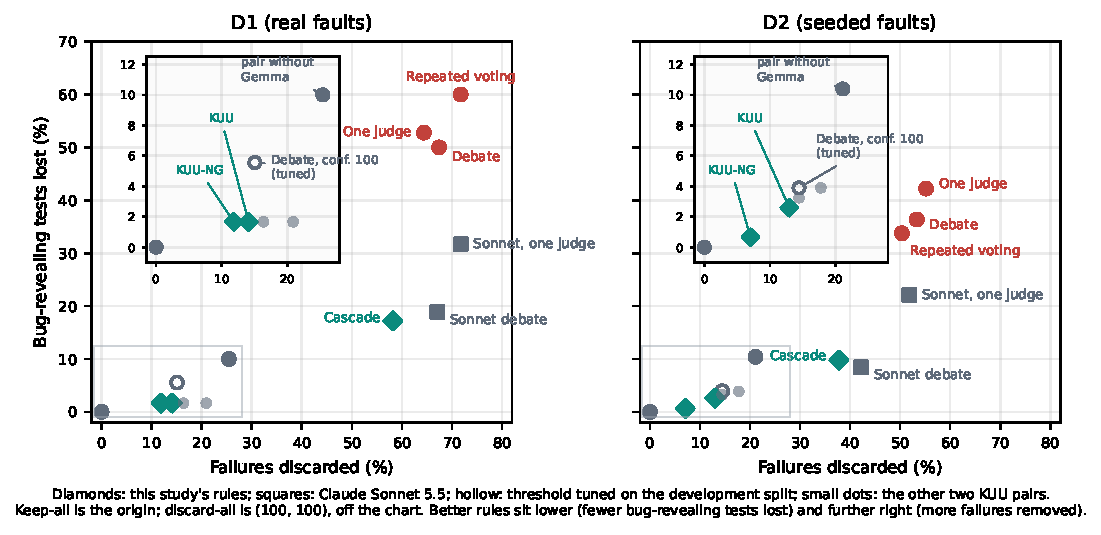
\includegraphics[width=0.8\textwidth]{figures/fig_pareto.pdf}
\caption{Share of failures each rule discards against the share of bug-revealing tests it loses (post hoc, descriptive). Insets enlarge the low-loss corner. Diamonds: this study's rules; squares: the frontier judge; the hollow point is the only rule with a threshold tuned on the development split.}\label{fig:tradeoff}
\end{figure*}

\par\medskip\noindent\begin{minipage}{\columnwidth}{\footnotesize\refstepcounter{table}\label{tab:rates}\textbf{Table~\thetable}\enspace Rates on a common scale (D-113), D-110's instance sets (D1-test \V{rv11:D1:n_instances}, D2 \V{rv11:D2:n_instances}). BA: balanced accuracy. FA: test faults kept per bug-revealing test kept at an assumed \PF{} prevalence of 5\%.\par}\smallskip
{\noindent\scriptsize\setlength{\tabcolsep}{2.5pt}
\resizebox{\columnwidth}{!}{\begin{tabular}{@{}l r r r r r r r@{}}
\toprule
 & \multicolumn{3}{c}{D1-test} & \multicolumn{3}{c}{D2} & \\
\cmidrule(lr){2-4}\cmidrule(lr){5-7}
Rule & TPR & TNR & BA & TPR & TNR & BA & FA$_{5\%}$ \\
\midrule
Keep-all & \V{rv11:D1:rules:KA:tpr} & \V{rv11:D1:rules:KA:tnr} & \V{rv11:D1:rules:KA:ba} & \V{rv11:D2:rules:KA:tpr} & \V{rv11:D2:rules:KA:tnr} & \V{rv11:D2:rules:KA:ba} & \V{rv11:D2:rules:KA:at_prevalence:0.0500:false_alarms_per_kept_pf@1} \\
R0 & \V{rv11:D1:rules:R0:tpr} & \V{rv11:D1:rules:R0:tnr} & \V{rv11:D1:rules:R0:ba} & \V{rv11:D2:rules:R0:tpr} & \V{rv11:D2:rules:R0:tnr} & \V{rv11:D2:rules:R0:ba} & \V{rv11:D2:rules:R0:at_prevalence:0.0500:false_alarms_per_kept_pf@1} \\
M1 J1 & \V{rv11:D1:rules:J1|S1:tpr} & \V{rv11:D1:rules:J1|S1:tnr} & \V{rv11:D1:rules:J1|S1:ba} & \V{rv11:D2:rules:J1|S1:tpr} & \V{rv11:D2:rules:J1|S1:tnr} & \V{rv11:D2:rules:J1|S1:ba} & \V{rv11:D2:rules:J1|S1:at_prevalence:0.0500:false_alarms_per_kept_pf@1} \\
M1 SC & \V{rv11:D1:rules:SC|S1:tpr} & \V{rv11:D1:rules:SC|S1:tnr} & \V{rv11:D1:rules:SC|S1:ba} & \V{rv11:D2:rules:SC|S1:tpr} & \V{rv11:D2:rules:SC|S1:tnr} & \V{rv11:D2:rules:SC|S1:ba} & \V{rv11:D2:rules:SC|S1:at_prevalence:0.0500:false_alarms_per_kept_pf@1} \\
M1 DEB & \V{rv11:D1:rules:DEB|S1:tpr} & \V{rv11:D1:rules:DEB|S1:tnr} & \V{rv11:D1:rules:DEB|S1:ba} & \V{rv11:D2:rules:DEB|S1:tpr} & \V{rv11:D2:rules:DEB|S1:tnr} & \V{rv11:D2:rules:DEB|S1:ba} & \V{rv11:D2:rules:DEB|S1:at_prevalence:0.0500:false_alarms_per_kept_pf@1} \\
M1 DEB, confidence 100 (tuned) & \V{rv11:D1:rules:TAU|S1:tpr} & \V{rv11:D1:rules:TAU|S1:tnr} & \V{rv11:D1:rules:TAU|S1:ba} & \V{rv11:D2:rules:TAU|S1:tpr} & \V{rv11:D2:rules:TAU|S1:tnr} & \V{rv11:D2:rules:TAU|S1:ba} & \V{rv11:D2:rules:TAU|S1:at_prevalence:0.0500:false_alarms_per_kept_pf@1} \\
Cross-family 2-of-3 & \V{rv11:D1:rules:MAJ3|S1:tpr} & \V{rv11:D1:rules:MAJ3|S1:tnr} & \V{rv11:D1:rules:MAJ3|S1:ba} & \V{rv11:D2:rules:MAJ3|S1:tpr} & \V{rv11:D2:rules:MAJ3|S1:tnr} & \V{rv11:D2:rules:MAJ3|S1:ba} & \V{rv11:D2:rules:MAJ3|S1:at_prevalence:0.0500:false_alarms_per_kept_pf@1} \\
KUU & \V{rv11:D1:rules:KUU|S1:tpr} & \V{rv11:D1:rules:KUU|S1:tnr} & \V{rv11:D1:rules:KUU|S1:ba} & \V{rv11:D2:rules:KUU|S1:tpr} & \V{rv11:D2:rules:KUU|S1:tnr} & \V{rv11:D2:rules:KUU|S1:ba} & \V{rv11:D2:rules:KUU|S1:at_prevalence:0.0500:false_alarms_per_kept_pf@1} \\
KUU-NG & \V{rv11:D1:rules:KUUNG|S1:tpr} & \V{rv11:D1:rules:KUUNG|S1:tnr} & \V{rv11:D1:rules:KUUNG|S1:ba} & \V{rv11:D2:rules:KUUNG|S1:tpr} & \V{rv11:D2:rules:KUUNG|S1:tnr} & \V{rv11:D2:rules:KUUNG|S1:ba} & \V{rv11:D2:rules:KUUNG|S1:at_prevalence:0.0500:false_alarms_per_kept_pf@1} \\
Cascade & \V{rv11:D1:rules:CAS|S1:tpr} & \V{rv11:D1:rules:CAS|S1:tnr} & \V{rv11:D1:rules:CAS|S1:ba} & \V{rv11:D2:rules:CAS|S1:tpr} & \V{rv11:D2:rules:CAS|S1:tnr} & \V{rv11:D2:rules:CAS|S1:ba} & \V{rv11:D2:rules:CAS|S1:at_prevalence:0.0500:false_alarms_per_kept_pf@1} \\
Sonnet J1 & \V{rv11:D1:rules:J1|S1|SON:tpr} & \V{rv11:D1:rules:J1|S1|SON:tnr} & \V{rv11:D1:rules:J1|S1|SON:ba} & \V{rv11:D2:rules:J1|S1|SON:tpr} & \V{rv11:D2:rules:J1|S1|SON:tnr} & \V{rv11:D2:rules:J1|S1|SON:ba} & \V{rv11:D2:rules:J1|S1|SON:at_prevalence:0.0500:false_alarms_per_kept_pf@1} \\
Sonnet DEB & \V{rv11:D1:rules:DEB|S1|SON:tpr} & \V{rv11:D1:rules:DEB|S1|SON:tnr} & \V{rv11:D1:rules:DEB|S1|SON:ba} & \V{rv11:D2:rules:DEB|S1|SON:tpr} & \V{rv11:D2:rules:DEB|S1|SON:tnr} & \V{rv11:D2:rules:DEB|S1|SON:ba} & \V{rv11:D2:rules:DEB|S1|SON:at_prevalence:0.0500:false_alarms_per_kept_pf@1} \\
\bottomrule
\end{tabular}}
\par}\end{minipage}\par\medskip

\noindent\textit{Reading.} KUU keeps almost every bug-revealing test but removes only a minority of test faults, so its balanced accuracy on D2 (\V{rv11:D2:rules:KUU|S1:ba}, 95\% CI \V{rv11:D2:rules:KUU|S1:ba_ci95}) is below M1 DEB's (\V{rv11:D2:rules:DEB|S1:ba}, \V{rv11:D2:rules:DEB|S1:ba_ci95}) and far below the cascade's (\V{rv11:D2:rules:CAS|S1:ba}, \V{rv11:D2:rules:CAS|S1:ba_ci95}). On D2, KUU-NG discards \V{rv11:reviewer_figures:kuung_share_discarded_D2@pct1} of failures, KUU \V{rv11:reviewer_figures:kuu_share_discarded_D2@pct1} and the cascade \V{rv11:reviewer_figures:cascade_share_discarded_D2@pct1}. At the D1-test labelled prevalence (\V{rv11:D1:population_pf_prevalence@3}) KUU keeps \V{rv11:D1:rules:KUU|S1:at_prevalence:0.1685:false_alarms_per_kept_pf@1} test faults per bug-revealing test kept, keep-all \V{rv11:D1:rules:KA:at_prevalence:0.1685:false_alarms_per_kept_pf@1}. Scoring invalid outputs as keep instead of \TF{} changes no single-judge arm's balanced accuracy by more than \V{der:inv keep max dBA@3}. Sonnet's DEB balanced accuracy on D1 minus D2 is \V{rv11:sonnet_e9_vs_e9b:DEB|S1|SON:ba:d1_minus_d2} (\V{rv11:sonnet_e9_vs_e9b:DEB|S1|SON:ba:d1_minus_d2_ci95}; unpaired, different instances and fault process, not a method effect).

\par\medskip\noindent\begin{minipage}{\columnwidth}{\footnotesize\refstepcounter{table}\label{tab:ranking}\textbf{Table~\thetable}\enspace Triage as ranking (D-114). Scores: stated confidence in the stated label for J1 and DEB, \PF{} vote share for SC, the number of non-\TF{} votes for the panels. Top 20\%: share of \PF{} tests (test) and of bugs with a \PF{} test (bug) found in the highest-scored 20\% of failures; random inspection finds 20\% of tests.\par}\smallskip
{\noindent\scriptsize\setlength{\tabcolsep}{2.5pt}
\resizebox{\columnwidth}{!}{\begin{tabular}{@{}l l l r r r r@{}}
\toprule
 & \multicolumn{2}{c}{AUROC [95\% CI]} & \multicolumn{2}{c}{D1 top 20\%} & \multicolumn{2}{c}{D2 top 20\%} \\
\cmidrule(lr){2-3}\cmidrule(lr){4-5}\cmidrule(lr){6-7}
Score & D1-test & D2 & test & bug & test & bug \\
\midrule
Keep-all & \V{rv13:D1:rules:KA:auroc} & \V{rv13:D2:rules:KA:auroc} & \V{rv13:D1:rules:KA:inspection:top20:recall@2} & \V{rv13:D1:rules:KA:inspection:top20:bug_recall@2} & \V{rv13:D2:rules:KA:inspection:top20:recall@2} & \V{rv13:D2:rules:KA:inspection:top20:bug_recall@2} \\
M1 J1 & \V{rv13:D1:rules:J1|S1:auroc} \V{rv13:D1:rules:J1|S1:auroc_ci95} & \V{rv13:D2:rules:J1|S1:auroc} \V{rv13:D2:rules:J1|S1:auroc_ci95} & \V{rv13:D1:rules:J1|S1:inspection:top20:recall@2} & \V{rv13:D1:rules:J1|S1:inspection:top20:bug_recall@2} & \V{rv13:D2:rules:J1|S1:inspection:top20:recall@2} & \V{rv13:D2:rules:J1|S1:inspection:top20:bug_recall@2} \\
M1 SC & \V{rv13:D1:rules:SC|S1:auroc} \V{rv13:D1:rules:SC|S1:auroc_ci95} & \V{rv13:D2:rules:SC|S1:auroc} \V{rv13:D2:rules:SC|S1:auroc_ci95} & \V{rv13:D1:rules:SC|S1:inspection:top20:recall@2} & \V{rv13:D1:rules:SC|S1:inspection:top20:bug_recall@2} & \V{rv13:D2:rules:SC|S1:inspection:top20:recall@2} & \V{rv13:D2:rules:SC|S1:inspection:top20:bug_recall@2} \\
M1 DEB & \V{rv13:D1:rules:DEB|S1:auroc} \V{rv13:D1:rules:DEB|S1:auroc_ci95} & \V{rv13:D2:rules:DEB|S1:auroc} \V{rv13:D2:rules:DEB|S1:auroc_ci95} & \V{rv13:D1:rules:DEB|S1:inspection:top20:recall@2} & \V{rv13:D1:rules:DEB|S1:inspection:top20:bug_recall@2} & \V{rv13:D2:rules:DEB|S1:inspection:top20:recall@2} & \V{rv13:D2:rules:DEB|S1:inspection:top20:bug_recall@2} \\
KUU panel votes & \V{rv13:D1:rules:KUU|S1:auroc} \V{rv13:D1:rules:KUU|S1:auroc_ci95} & \V{rv13:D2:rules:KUU|S1:auroc} \V{rv13:D2:rules:KUU|S1:auroc_ci95} & \V{rv13:D1:rules:KUU|S1:inspection:top20:recall@2} & \V{rv13:D1:rules:KUU|S1:inspection:top20:bug_recall@2} & \V{rv13:D2:rules:KUU|S1:inspection:top20:recall@2} & \V{rv13:D2:rules:KUU|S1:inspection:top20:bug_recall@2} \\
KUU-NG panel votes & \V{rv13:D1:rules:KUUNG|S1:auroc} \V{rv13:D1:rules:KUUNG|S1:auroc_ci95} & \V{rv13:D2:rules:KUUNG|S1:auroc} \V{rv13:D2:rules:KUUNG|S1:auroc_ci95} & \V{rv13:D1:rules:KUUNG|S1:inspection:top20:recall@2} & \V{rv13:D1:rules:KUUNG|S1:inspection:top20:bug_recall@2} & \V{rv13:D2:rules:KUUNG|S1:inspection:top20:recall@2} & \V{rv13:D2:rules:KUUNG|S1:inspection:top20:bug_recall@2} \\
Sonnet DEB & \V{rv13:D1:rules:DEB|S1|SON:auroc} \V{rv13:D1:rules:DEB|S1|SON:auroc_ci95} & \V{rv13:D2:rules:DEB|S1|SON:auroc} \V{rv13:D2:rules:DEB|S1|SON:auroc_ci95} & \V{rv13:D1:rules:DEB|S1|SON:inspection:top20:recall@2} & \V{rv13:D1:rules:DEB|S1|SON:inspection:top20:bug_recall@2} & \V{rv13:D2:rules:DEB|S1|SON:inspection:top20:recall@2} & \V{rv13:D2:rules:DEB|S1|SON:inspection:top20:bug_recall@2} \\
\bottomrule
\end{tabular}}
\par}\end{minipage}\par\medskip

\noindent\textit{Reading.} Confidence adds to the label for every judge (M1 DEB AUROC \V{rv13:D1:rules:DEB|S1:auroc} with confidence, \V{rv13:D1:rules:DEB|S1:auroc_label_only} from the label alone, D1). Test-level and bug-level recall need not agree: on D2 Sonnet's top 20\% are all \PF{} tests (precision \V{rv13:D2:rules:DEB|S1|SON:inspection:top20:precision@2}), yet they cover fewer bugs (\V{rv13:D2:rules:DEB|S1|SON:inspection:top20:bug_recall@2}) than random inspection (\V{rv13:D2:rules:KA:inspection:top20:bug_recall@2}), because its most confident \PF{} tests cluster in a few bugs. Reweighted to the D1-test labelled population (\PF{} share \V{rv13:D1:reweighting:weighted_pf_share@3}), the KUU panel's AUPRC is \V{rv13:D1:rules:KUU|S1:reweighted:auprc} against \V{rv13:D1:rules:KUU|S1:reweighted:auprc_random} for a random order and Sonnet DEB's \V{rv13:D1:rules:DEB|S1|SON:reweighted:auprc}; the reweighting assumes the sampled test faults represent their project's.

\par\medskip\noindent\begin{minipage}{\columnwidth}{\footnotesize\refstepcounter{table}\label{tab:learned}\textbf{Table~\thetable}\enspace Trained baselines (D-115, exploratory): logistic regression, leave-one-project-out on D1-test (pooled out-of-fold predictions, threshold 0.5 fixed in advance, nothing tuned), and one transfer to D2. Failure features: assertion or exception, exception family, deepest project frame, expected/actual values present. Votes: the KUU members' J1 votes.\par}\smallskip
{\noindent\scriptsize\setlength{\tabcolsep}{2.5pt}
\resizebox{\columnwidth}{!}{\begin{tabular}{@{}l r r l l r r@{}}
\toprule
 & \multicolumn{4}{c}{D1-test, leave one project out} & \multicolumn{2}{c}{D1 $\to$ D2} \\
\cmidrule(lr){2-5}\cmidrule(lr){6-7}
Model & TPR & TNR & BA [95\% CI] & AUROC [95\% CI] & BA & AUROC \\
\midrule
Failure features only (no LLM) & \V{rv14:lopo:features:tpr} & \V{rv14:lopo:features:tnr} & \V{rv14:lopo:features:ba} \V{rv14:lopo:features:ba_ci95} & \V{rv14:lopo:features:auroc} \V{rv14:lopo:features:auroc_ci95} & \V{rv14:transfer_D1_to_D2:features:ba} & \V{rv14:transfer_D1_to_D2:features:auroc} \\
Votes only & \V{rv14:lopo:votes:tpr} & \V{rv14:lopo:votes:tnr} & \V{rv14:lopo:votes:ba} \V{rv14:lopo:votes:ba_ci95} & \V{rv14:lopo:votes:auroc} \V{rv14:lopo:votes:auroc_ci95} & \V{rv14:transfer_D1_to_D2:votes:ba} & \V{rv14:transfer_D1_to_D2:votes:auroc} \\
Stacker (votes + features) & \V{rv14:lopo:stacker:tpr} & \V{rv14:lopo:stacker:tnr} & \V{rv14:lopo:stacker:ba} \V{rv14:lopo:stacker:ba_ci95} & \V{rv14:lopo:stacker:auroc} \V{rv14:lopo:stacker:auroc_ci95} & \V{rv14:transfer_D1_to_D2:stacker:ba} & \V{rv14:transfer_D1_to_D2:stacker:auroc} \\
Stacker + cross-generation & \V{rv14:lopo:stacker+cg:tpr} & \V{rv14:lopo:stacker+cg:tnr} & \V{rv14:lopo:stacker+cg:ba} \V{rv14:lopo:stacker+cg:ba_ci95} & \V{rv14:lopo:stacker+cg:auroc} \V{rv14:lopo:stacker+cg:auroc_ci95} & \V{rv14:transfer_D1_to_D2:stacker+cg:ba} & \V{rv14:transfer_D1_to_D2:stacker+cg:auroc} \\
KUU (no training) & \V{rv11:D1:rules:KUU|S1:tpr} & \V{rv11:D1:rules:KUU|S1:tnr} & \V{rv11:D1:rules:KUU|S1:ba} \V{rv11:D1:rules:KUU|S1:ba_ci95} & \V{rv13:D1:rules:KUU|S1:auroc} \V{rv13:D1:rules:KUU|S1:auroc_ci95} & \V{rv11:D2:rules:KUU|S1:ba} & \V{rv13:D2:rules:KUU|S1:auroc} \\
\bottomrule
\end{tabular}}
\par}\end{minipage}\par\medskip

\noindent\textit{Reading.} The failure features alone carry little signal across projects; a learned weighting of the three votes reaches a higher balanced accuracy than KUU but keeps fewer bug-revealing tests (TPR \V{rv14:lopo:votes:tpr} against \V{rv11:D1:rules:KUU|S1:tpr}), the trade-off a threshold moves along; the failure features and the cross-generation signal add nothing to the votes.

\par\medskip\noindent\begin{minipage}{\columnwidth}{\footnotesize\refstepcounter{table}\label{tab:kofn}\textbf{Table~\thetable}\enspace Discard when at least $k$ of three judges vote \TF{} (D-116): \PF{}-loss rate (1 $-$ TPR) / \TF{}-removal rate (TNR). $k=3$ of the KUU panel is KUU. Within-model: the first three of five SC samples.\par}\smallskip
{\noindent\scriptsize\setlength{\tabcolsep}{2.5pt}
\resizebox{\columnwidth}{!}{\begin{tabular}{@{}l l l l l l l@{}}
\toprule
 & \multicolumn{3}{c}{D1-test} & \multicolumn{3}{c}{D2} \\
\cmidrule(lr){2-4}\cmidrule(lr){5-7}
Triple & $k=1$ & $k=2$ & $k=3$ & $k=1$ & $k=2$ & $k=3$ \\
\midrule
KUU panel & \V{rv15:D1:triples:KUUpanel(M1,M2,E6b):k=1:pf_loss_rate@2}/\V{rv15:D1:triples:KUUpanel(M1,M2,E6b):k=1:tnr@2} & \V{rv15:D1:triples:KUUpanel(M1,M2,E6b):k=2:pf_loss_rate@2}/\V{rv15:D1:triples:KUUpanel(M1,M2,E6b):k=2:tnr@2} & \V{rv15:D1:triples:KUUpanel(M1,M2,E6b):k=3:pf_loss_rate@2}/\V{rv15:D1:triples:KUUpanel(M1,M2,E6b):k=3:tnr@2} & \V{rv15:D2:triples:KUUpanel(M1,M2,E6b):k=1:pf_loss_rate@2}/\V{rv15:D2:triples:KUUpanel(M1,M2,E6b):k=1:tnr@2} & \V{rv15:D2:triples:KUUpanel(M1,M2,E6b):k=2:pf_loss_rate@2}/\V{rv15:D2:triples:KUUpanel(M1,M2,E6b):k=2:tnr@2} & \V{rv15:D2:triples:KUUpanel(M1,M2,E6b):k=3:pf_loss_rate@2}/\V{rv15:D2:triples:KUUpanel(M1,M2,E6b):k=3:tnr@2} \\
KUU-NG panel & \V{rv15:D1:triples:KUU-NGpanel(M1,E6b,Llama):k=1:pf_loss_rate@2}/\V{rv15:D1:triples:KUU-NGpanel(M1,E6b,Llama):k=1:tnr@2} & \V{rv15:D1:triples:KUU-NGpanel(M1,E6b,Llama):k=2:pf_loss_rate@2}/\V{rv15:D1:triples:KUU-NGpanel(M1,E6b,Llama):k=2:tnr@2} & \V{rv15:D1:triples:KUU-NGpanel(M1,E6b,Llama):k=3:pf_loss_rate@2}/\V{rv15:D1:triples:KUU-NGpanel(M1,E6b,Llama):k=3:tnr@2} & \V{rv15:D2:triples:KUU-NGpanel(M1,E6b,Llama):k=1:pf_loss_rate@2}/\V{rv15:D2:triples:KUU-NGpanel(M1,E6b,Llama):k=1:tnr@2} & \V{rv15:D2:triples:KUU-NGpanel(M1,E6b,Llama):k=2:pf_loss_rate@2}/\V{rv15:D2:triples:KUU-NGpanel(M1,E6b,Llama):k=2:tnr@2} & \V{rv15:D2:triples:KUU-NGpanel(M1,E6b,Llama):k=3:pf_loss_rate@2}/\V{rv15:D2:triples:KUU-NGpanel(M1,E6b,Llama):k=3:tnr@2} \\
M1 within-model & \V{rv15:D1:triples:M1within-model(first3SCsamples):k=1:pf_loss_rate@2}/\V{rv15:D1:triples:M1within-model(first3SCsamples):k=1:tnr@2} & \V{rv15:D1:triples:M1within-model(first3SCsamples):k=2:pf_loss_rate@2}/\V{rv15:D1:triples:M1within-model(first3SCsamples):k=2:tnr@2} & \V{rv15:D1:triples:M1within-model(first3SCsamples):k=3:pf_loss_rate@2}/\V{rv15:D1:triples:M1within-model(first3SCsamples):k=3:tnr@2} & \V{rv15:D2:triples:M1within-model(first3SCsamples):k=1:pf_loss_rate@2}/\V{rv15:D2:triples:M1within-model(first3SCsamples):k=1:tnr@2} & \V{rv15:D2:triples:M1within-model(first3SCsamples):k=2:pf_loss_rate@2}/\V{rv15:D2:triples:M1within-model(first3SCsamples):k=2:tnr@2} & \V{rv15:D2:triples:M1within-model(first3SCsamples):k=3:pf_loss_rate@2}/\V{rv15:D2:triples:M1within-model(first3SCsamples):k=3:tnr@2} \\
M2 within-model & \V{rv15:D1:triples:M2within-model(first3SCsamples):k=1:pf_loss_rate@2}/\V{rv15:D1:triples:M2within-model(first3SCsamples):k=1:tnr@2} & \V{rv15:D1:triples:M2within-model(first3SCsamples):k=2:pf_loss_rate@2}/\V{rv15:D1:triples:M2within-model(first3SCsamples):k=2:tnr@2} & \V{rv15:D1:triples:M2within-model(first3SCsamples):k=3:pf_loss_rate@2}/\V{rv15:D1:triples:M2within-model(first3SCsamples):k=3:tnr@2} & \V{rv15:D2:triples:M2within-model(first3SCsamples):k=1:pf_loss_rate@2}/\V{rv15:D2:triples:M2within-model(first3SCsamples):k=1:tnr@2} & \V{rv15:D2:triples:M2within-model(first3SCsamples):k=2:pf_loss_rate@2}/\V{rv15:D2:triples:M2within-model(first3SCsamples):k=2:tnr@2} & \V{rv15:D2:triples:M2within-model(first3SCsamples):k=3:pf_loss_rate@2}/\V{rv15:D2:triples:M2within-model(first3SCsamples):k=3:tnr@2} \\
\bottomrule
\end{tabular}}
\par}\end{minipage}\par\medskip

\par\medskip\noindent\begin{minipage}{\columnwidth}{\footnotesize\refstepcounter{table}\label{tab:revmisc}\textbf{Table~\thetable}\enspace Risk-targeted threshold (D-117), cross-generation signal (D-118), sample-size planning (D-119), integrity checks (D-120), the leakage guard's selection (D-121) and label-noise sensitivity (D-121).\par}\smallskip
{\noindent\scriptsize\setlength{\tabcolsep}{3pt}
\resizebox{\columnwidth}{!}{\begin{tabular}{@{}l r@{}}
\toprule
Quantity & Value \\
\midrule
\multicolumn{2}{@{}l}{\textit{Risk-targeted threshold, $\alpha=0.05$ on \PF{} tests, calibrated on D1, evaluated on D2 (a heuristic: see text)}} \\
KUU panel + DEB confidence: D2 \PF{}-loss / \TF{}-removal & \V{rv16:panels:KUU:thresholds:tests_alpha0.05:D2_evaluation:pf_loss_rate} / \V{rv16:panels:KUU:thresholds:tests_alpha0.05:D2_evaluation:tnr} \\
KUU-NG panel + DEB confidence: D2 \PF{}-loss / \TF{}-removal & \V{rv16:panels:KUU-NG:thresholds:tests_alpha0.05:D2_evaluation:pf_loss_rate} / \V{rv16:panels:KUU-NG:thresholds:tests_alpha0.05:D2_evaluation:tnr} \\
\multicolumn{2}{@{}l}{\textit{Cross-generation agreement (buggy version only): AUROC}} \\
D1-test / D2 & \V{rv17:D1:auroc_cg} \V{rv17:D1:auroc_cg_ci95} / \V{rv17:D2:auroc_cg} \V{rv17:D2:auroc_cg_ci95} \\
\multicolumn{2}{@{}l}{\textit{Bugs needed for an MDE of 0.08 (0.05) at 80\% power, $\alpha=0.05$; now \V{rv18:tests:H3a:n0_bugs} bugs}} \\
H3a (DEB vs SC) & \V{rv18:tests:H3a:by_mde:0.08:bugs_alpha_005} (\V{rv18:tests:H3a:by_mde:0.05:bugs_alpha_005}), \V{rv18:tests:H3a:by_mde:0.08:multiplier_alpha_005@1}$\times$ \\
H2a (Javadoc) & \V{rv18:tests:H2a:by_mde:0.08:bugs_alpha_005} (\V{rv18:tests:H2a:by_mde:0.05:bugs_alpha_005}) \\
\multicolumn{2}{@{}l}{\textit{Integrity}} \\
Holm families reproduced from stored $p$ & \V{der:holm all match} \V{der:holm families} \\
\multicolumn{2}{@{}l}{\textit{Leakage-guard aborts among judged D2 instances}} \\
Aborted (\PF{}, matched the injected line) & \V{rv110:guard:D2:aborted_at_S1_any_run} of \V{rv110:guard:D2:judged} (\V{rv110:guard:D2:aborted_by_label:PF}, \V{rv110:guard:D2:aborted_matched_kind:themutatedline}) \\
Scored \PF{} prevalence with / without aborts & \V{rv110:guard:D2:judged_with_aborts:pf_prevalence_scored} / \V{rv110:guard:D2:judged_without_aborts:pf_prevalence_scored} \\
\multicolumn{2}{@{}l}{\textit{Label noise: execution-\TF{} assertion failures relabelled \PF{} (median BA over 1{,}000 draws)}} \\
D2 KUU: none / audit rate \V{rv110:noise_model:audit_rate:value@2} / 0.10 & \V{rv110:noise:D2:no_noise:KUU|S1:ba} / \V{rv110:noise:D2:rules:q=0.0400:KUU|S1:ba:median} / \V{rv110:noise:D2:rules:q=0.1000:KUU|S1:ba:median} \\
D1 Sonnet DEB: none / audit rate / 0.10 & \V{rv110:noise:D1:no_noise:DEB|S1|SON:ba} / \V{rv110:noise:D1:rules:q=0.0400:DEB|S1|SON:ba:median} / \V{rv110:noise:D1:rules:q=0.1000:DEB|S1|SON:ba:median} \\
\bottomrule
\end{tabular}}
\par}\end{minipage}\par\medskip

\noindent\textit{Reading.} The risk-targeted threshold is not a conformal guarantee: its calibration set (D1) is the data KUU was designed on and is not exchangeable with D2 (different fault process and prevalence). The two panels show why this matters: calibrated to the same target, one stays within it on D2 and the other does not. Cross-generation agreement is a signal for seeded faults but not for real ones. The planning numbers assume the bootstrap standard error falls as one over the square root of the number of bugs; they are guidance, not a power guarantee. Every interval in the paper resamples bugs (the label-audit $\kappa$ uses 2{,}000 resamples, as fixed in D-82). The guard removed the D2 instances whose evidence showed the injected line, so the scored D2 set under-represents faults visible in the test evidence. The label-noise model is hypothetical (the audit rate comes from development-split items rated by the authors); it moves no rule's balanced accuracy enough to change the order of the rules.

\par\medskip\noindent\begin{minipage}{\columnwidth}{\footnotesize\refstepcounter{table}\label{tab:gates}\textbf{Table~\thetable}\enspace Development gates of every local judge (dev pilot, \V{devgate:n_instances} instances): G-a output validity, G-b evidence citation, G-c, G-d one-shot F1 above both trivial baselines (R0: \V{rv2:gates:M1(Qwen3.59B):R0_f1_dev}). Sonnet and the 35B judge were not gated.\par}\smallskip
{\noindent\scriptsize\setlength{\tabcolsep}{4pt}
\resizebox{\columnwidth}{!}{\begin{tabular}{@{}l c c c c r@{}}
\toprule
Judge & G-a & G-b & G-c & G-d & J1 F1 (dev) \\
\midrule
M1 Qwen3.5 9B & \V{der:gate M1 G_a} & \V{der:gate M1 G_b} & \V{der:gate M1 G_c} & \V{der:gate M1 G_d} & \V{rv2:gates:M1(Qwen3.59B):J1_f1_dev} \\
M2 Gemma~4 12B & \V{der:gate M2 G_a} & \V{der:gate M2 G_b} & \V{der:gate M2 G_c} & \V{der:gate M2 G_d} & \V{rv2:gates:M2(Gemma412B):J1_f1_dev} \\
M3 Ministral~3 14B & \V{der:gate M3 G_a} & \V{der:gate M3 G_b} & \V{der:gate M3 G_c} & \V{der:gate M3 G_d} & \V{rv2:gates:E6b(Ministral314B):J1_f1_dev} \\
NG Llama~3.1 8B & \V{der:gate NG G_a} & \V{der:gate NG G_b} & \V{der:gate NG G_c} & \V{der:gate NG G_d} & \V{rv2:gates:NG(Llama3.18B):J1_f1_dev} \\
\bottomrule
\end{tabular}}
\par}\end{minipage}\par\medskip

\par\medskip\noindent\begin{minipage}{\columnwidth}{\footnotesize\refstepcounter{table}\label{tab:wp2}\textbf{Table~\thetable}\enspace Local runs added in response to review (D-123 to D-127, exploratory; own server, frozen prompts, the D-109 stopping rule). (a) The \V{der:tf176 n} D1-test test faults the 1:2 sample left out, judged by M1, M2, M3 and NG and pooled with the sampled ones; precision and false alarms are at the natural prevalence, with no weights. (b) M1's one-shot judge at temperature 0. (c) M1's one-shot judge with thinking enabled (context \V{cfgth:spec_patch:num_ctx@int} tokens, output cap \V{cfgth:max_tokens@int}, thinking included); Ollama caps total output, not thinking, so the run is not token-matched by construction. (d) M1 DEB, eight replicates (three committed, five new).\par}\smallskip
{\noindent\scriptsize\setlength{\tabcolsep}{3pt}
\resizebox{\columnwidth}{!}{\begin{tabular}{@{}l r@{}}
\toprule
Quantity & Value \\
\midrule
\multicolumn{2}{@{}l}{\textit{(a) All judgeable D1-test test faults: \V{rv2:tf296:n_tf_judged} of \V{der:d1 test TF labelled}, with the \V{rv2:tf296:n_pf} \PF{}}} \\
KUU: TNR all [95\% CI]; sampled / new & \V{rv2:tf296:rules:KUU:all:tnr} \V{rv2:tf296:rules:KUU:all:tnr_ci95}; \V{rv2:tf296:rules:KUU:tnr_original_sample} / \V{rv2:tf296:rules:KUU:tnr_new_176} \\
KUU-NG: TNR all; sampled / new & \V{rv2:tf296:rules:KUU-NG:all:tnr} \V{rv2:tf296:rules:KUU-NG:all:tnr_ci95}; \V{rv2:tf296:rules:KUU-NG:tnr_original_sample} / \V{rv2:tf296:rules:KUU-NG:tnr_new_176} \\
M1 J1: TNR all; sampled / new & \V{rv2:tf296:rules:M1J1:all:tnr} \V{rv2:tf296:rules:M1J1:all:tnr_ci95}; \V{rv2:tf296:rules:M1J1:tnr_original_sample} / \V{rv2:tf296:rules:M1J1:tnr_new_176} \\
Precision: keep-all / KUU / KUU-NG / M1 J1 & \V{rv2:tf296:rules:Keepall:all:precision} / \V{rv2:tf296:rules:KUU:all:precision} / \V{rv2:tf296:rules:KUU-NG:all:precision} / \V{rv2:tf296:rules:M1J1:all:precision} \\
Test faults per kept \PF{} test: keep-all / KUU / KUU-NG & \V{rv2:tf296:rules:Keepall:all:false_alarms_per_kept_pf@1} / \V{rv2:tf296:rules:KUU:all:false_alarms_per_kept_pf@1} / \V{rv2:tf296:rules:KUU-NG:all:false_alarms_per_kept_pf@1} \\
\multicolumn{2}{@{}l}{\textit{(b) Greedy one-shot judge, D1-test (\V{rv11:D1:n_instances} instances)}} \\
BA / F1 / MCC at temperature \V{cfgt0:temperature@1} & \V{rv2:greedy:temperature_0:50:ba} / \V{rv2:greedy:temperature_0:50:f1} / \V{rv2:greedy:temperature_0:50:mcc} \\
BA / F1 / MCC at \V{frozen:frozen_models:M1:temperature:judges@1} (three replicates) & \V{rv11:D1:rules:J1|S1:ba} / \V{rv11:D1:rules:J1|S1:f1} / \V{rv11:D1:rules:J1|S1:mcc} \\
\multicolumn{2}{@{}l}{\textit{(c) Thinking-enabled one-shot judge (M1, one run), D1-test (\V{rv2:think:heldout:60:n} instances)}} \\
BA / F1 / MCC & \V{rv2:think:heldout:60:ba} / \V{rv2:think:heldout:60:f1} / \V{rv2:think:heldout:60:mcc} \\
TPR / TNR; \PF{} tests lost; no answer (output cap) & \V{rv2:think:heldout:60:tpr} / \V{rv2:think:heldout:60:tnr}; \V{rv2:think:heldout:60:FN@0}; \V{rv2:think:heldout:60:invalid@0} \\
Consumed tokens per instance (M1 DEB \V{rv2:think:deb_consumed_tokens_per_instance_table@0}) & \V{rv2:think:heldout:60:consumed_tokens_per_instance@0} (\V{rv2:think:heldout:60:ratio_to_deb_tokens@2}$\times$; not token-matched) \\
BA of M1 DEB / SC-T (three runs, mean) & \V{rv11:D1:rules:DEB|S1:ba} / \V{rv11:D1:rules:SC-T|S1:ba} \\
\multicolumn{2}{@{}l}{\textit{(d) Debate replicates: \V{rv2:deb8:n_replicates} runs of M1 DEB on D1-test}} \\
F1 min--max (range, SD) & \V{rv2:deb8:spread:f1:min}--\V{rv2:deb8:spread:f1:max} (\V{rv2:deb8:spread:f1:range}, \V{rv2:deb8:spread:f1:sd}) \\
BA min--max (range) & \V{rv2:deb8:spread:ba:min}--\V{rv2:deb8:spread:ba:max} (\V{rv2:deb8:spread:ba:range}) \\
MCC min--max & \V{rv2:deb8:spread:mcc:min}--\V{rv2:deb8:spread:mcc:max} \\
\bottomrule
\end{tabular}}
\par}\end{minipage}\par\medskip

\par\medskip\noindent\begin{minipage}{\columnwidth}{\footnotesize\refstepcounter{table}\label{tab:think}\textbf{Table~\thetable}\enspace Thinking-enabled M1 one-shot judge, followed up as KUU was (D-130). Same configuration in every run (Table~\ref{tab:wp2}c); the development gate, the D2 hypotheses (one Holm family, paired bug-level bootstrap, 10{,}000 resamples) and the wording rule for this paper were fixed in advance in the version-controlled decision log. Primary coding: an output cut off by the cap scores \TF{}; the other codings are sensitivity only. Descriptive rows use D-110's common sets and are not tests. Tokens: Ollama prompt plus generated tokens, thinking included; not token-matched to debate.\par}\smallskip
{\noindent\scriptsize\setlength{\tabcolsep}{3pt}
\resizebox{\columnwidth}{!}{\begin{tabular}{@{}l r@{}}
\toprule
Quantity & Value \\
\midrule
\multicolumn{2}{@{}l}{\textit{(a) Development gate (dev pilot, \V{tk:gate:n_instances@int} labelled instances), as applied to M1}} \\
G-a valid outputs (needs $\geq$ 98\%) & \V{tk:gate:G_a_valid_rate:J1@pct1} (\V{tk:gate:G_a_runaway_D39:J1:invalid_length@int} cut off by the cap) \\
G-d J1 F1 vs best trivial rule (R0); thinking-disabled M1 & \V{tk:gate:G_d_detail:J1_f1} vs \V{tk:gate:G_d_detail:R0_f1}; \V{tk:gate:m1_original:J1_f1} \\
\multicolumn{2}{@{}l}{\textit{(b) D2 confirmation (\V{tk:d2:confirmatory:n_instances@int} instances, \V{tk:d2:confirmatory:n_bugs@int} bugs), thinking J1 vs M1 DEB}} \\
HT-1 $\Delta$MCC [95\% CI]; $p_\mathrm{Holm}$ & \V{tk:d2:confirmatory:HT-1:delta} \V{tk:d2:confirmatory:HT-1:ci95}; \V{tk:d2:confirmatory:HT-1:p_holm} \\
HT-2 $\Delta$\PF{} tests lost [95\% CI]; $p_\mathrm{Holm}$ & \V{tk:d2:confirmatory:HT-2:delta@int} \V{tk:d2:confirmatory:HT-2:ci95@ci0}; \V{tk:d2:confirmatory:HT-2:p_holm} \\
Cut off by the cap; HT-1 / HT-2 $\Delta$ if kept & \V{tk:d2:capped@int}; \V{tk:d2:policies:keep:hypotheses:HT-1:delta} / \V{tk:d2:policies:keep:hypotheses:HT-2:delta@int} \\
HT-1 / HT-2 $\Delta$ if excluded & \V{tk:d2:policies:exclude:hypotheses:HT-1:delta} / \V{tk:d2:policies:exclude:hypotheses:HT-2:delta@int} \\
\multicolumn{2}{@{}l}{\textit{(c) D2, descriptive: BA / TPR / TNR; \PF{} tests lost; bugs lost}} \\
Thinking M1 J1 & \V{tk:d2:descriptive:ThinkingM1J1:ba} / \V{tk:d2:descriptive:ThinkingM1J1:tpr} / \V{tk:d2:descriptive:ThinkingM1J1:tnr}; \V{tk:d2:descriptive:ThinkingM1J1:pf_lost@int}; \V{tk:d2:descriptive:ThinkingM1J1:bugs_lost@int} \\
M1 DEB & \V{tk:d2:descriptive:M1DEB:ba} / \V{tk:d2:descriptive:M1DEB:tpr} / \V{tk:d2:descriptive:M1DEB:tnr}; \V{tk:d2:descriptive:M1DEB:pf_lost@int}; \V{tk:d2:descriptive:M1DEB:bugs_lost@int} \\
KUU & \V{tk:d2:descriptive:KUU:ba} / \V{tk:d2:descriptive:KUU:tpr} / \V{tk:d2:descriptive:KUU:tnr}; \V{tk:d2:descriptive:KUU:pf_lost@int}; \V{tk:d2:descriptive:KUU:bugs_lost@int} \\
KUU-NG & \V{tk:d2:descriptive:KUU-NG:ba} / \V{tk:d2:descriptive:KUU-NG:tpr} / \V{tk:d2:descriptive:KUU-NG:tnr}; \V{tk:d2:descriptive:KUU-NG:pf_lost@int}; \V{tk:d2:descriptive:KUU-NG:bugs_lost@int} \\
Cascade & \V{tk:d2:descriptive:Cascade:ba} / \V{tk:d2:descriptive:Cascade:tpr} / \V{tk:d2:descriptive:Cascade:tnr}; \V{tk:d2:descriptive:Cascade:pf_lost@int}; \V{tk:d2:descriptive:Cascade:bugs_lost@int} \\
Sonnet DEB (frontier reference) & \V{tk:d2:descriptive:SonnetDEB:ba} / \V{tk:d2:descriptive:SonnetDEB:tpr} / \V{tk:d2:descriptive:SonnetDEB:tnr}; \V{tk:d2:descriptive:SonnetDEB:pf_lost@int}; \V{tk:d2:descriptive:SonnetDEB:bugs_lost@int} \\
\PF{} tests lost by thinking J1 but kept by KUU; the reverse & \V{tk:d2:kuu_vs_thinking:pf_lost_by_thinking_kept_by_kuu@int}; \V{tk:d2:kuu_vs_thinking:pf_lost_by_kuu_kept_by_thinking@int} \\
\multicolumn{2}{@{}l}{\textit{(d) D1-test, three runs (replicates 60, 63, 64; exploratory, found on these data)}} \\
BA per run & \V{tk:d1:runs:60:ba} / \V{tk:d1:runs:63:ba} / \V{tk:d1:runs:64:ba} \\
MCC per run & \V{tk:d1:runs:60:mcc} / \V{tk:d1:runs:63:mcc} / \V{tk:d1:runs:64:mcc} \\
F1 range (M1 DEB, eight runs) & \V{tk:d1:summary:f1:min}--\V{tk:d1:summary:f1:max} (\V{tk:d1:deb_eight_runs:f1:min}--\V{tk:d1:deb_eight_runs:f1:max}) \\
\PF{} tests lost per run (of \V{sum:prevalence:PF}); cut off by the cap & \V{tk:d1:runs:60:pf_lost@int} / \V{tk:d1:runs:63:pf_lost@int} / \V{tk:d1:runs:64:pf_lost@int}; \V{tk:d1:runs:60:capped@int} / \V{tk:d1:runs:63:capped@int} / \V{tk:d1:runs:64:capped@int} \\
Tokens per instance, D1 mean / D2 (M1 DEB on D1) & \V{tk:d1:summary:tokens_per_instance:mean@0} / \V{tk:d2:tokens_per_instance@0} (\V{tk:deb_tokens_per_instance_D1@0}) \\
\bottomrule
\end{tabular}}
\par}\end{minipage}\par\medskip

\par\medskip\noindent\begin{minipage}{\columnwidth}{\footnotesize\refstepcounter{table}\label{tab:localcas}\textbf{Table~\thetable}\enspace Fully local cascade (D-132, \emph{post hoc} on both sets, zero calls): KUU's unanimous votes decide; any disagreement goes to the logged thinking-enabled M1 J1 (Table~\ref{tab:think}), whose valid label decides, and an invalid or capped answer keeps the test. One rule, fixed in advance in the version-controlled decision log; no other variant was computed. Local minus Sonnet cascade on D2: $\Delta$BA \V{lc:D2:runs:62:local_minus_sonnet_cascade:ba:delta} \V{lc:D2:runs:62:local_minus_sonnet_cascade:ba:ci95}, $\Delta$MCC \V{lc:D2:runs:62:local_minus_sonnet_cascade:mcc:delta} \V{lc:D2:runs:62:local_minus_sonnet_cascade:mcc:ci95} (paired bug-level bootstrap, descriptive, no test). Lost: \PF{} tests lost; bugs: bugs with a \PF{} test and none kept; disc.: share of failures discarded. To be confirmed on fresh real faults (journal plan).\par}\smallskip
{\noindent\scriptsize\setlength{\tabcolsep}{2.5pt}
\resizebox{\columnwidth}{!}{\begin{tabular}{@{}l rrrrrrrr@{}}
\toprule
Rule & F1 & MCC & BA & TPR & TNR & Lost & Bugs & Disc. \\
\midrule
\multicolumn{9}{@{}l}{\textit{D2 (\V{lc:D2:n_instances@int} instances, \V{lc:D2:n_bugs@int} bugs; \V{lc:D2:share_escalated@pct0} reach Tier~2)}} \\
Fully local cascade & \V{lc:D2:runs:62:local_cascade:f1} & \V{lc:D2:runs:62:local_cascade:mcc} & \V{lc:D2:runs:62:local_cascade:ba} & \V{lc:D2:runs:62:local_cascade:tpr} & \V{lc:D2:runs:62:local_cascade:tnr} & \V{lc:D2:runs:62:local_cascade:pf_lost@0} & \V{lc:D2:runs:62:local_cascade:bugs_lost@0} & \V{lc:D2:runs:62:local_cascade:share_discarded@pct0} \\
Thinking M1 J1 alone & \V{lc:D2:runs:62:thinking_alone:f1} & \V{lc:D2:runs:62:thinking_alone:mcc} & \V{lc:D2:runs:62:thinking_alone:ba} & \V{lc:D2:runs:62:thinking_alone:tpr} & \V{lc:D2:runs:62:thinking_alone:tnr} & \V{lc:D2:runs:62:thinking_alone:pf_lost@0} & \V{lc:D2:runs:62:thinking_alone:bugs_lost@0} & \V{lc:D2:runs:62:thinking_alone:share_discarded@pct0} \\
KUU & \V{lc:D2:comparators:KUU:f1} & \V{lc:D2:comparators:KUU:mcc} & \V{lc:D2:comparators:KUU:ba} & \V{lc:D2:comparators:KUU:tpr} & \V{lc:D2:comparators:KUU:tnr} & \V{lc:D2:comparators:KUU:pf_lost@0} & \V{lc:D2:comparators:KUU:bugs_lost@0} & \V{lc:D2:comparators:KUU:share_discarded@pct0} \\
Sonnet cascade & \V{lc:D2:comparators:Sonnetcascade:f1} & \V{lc:D2:comparators:Sonnetcascade:mcc} & \V{lc:D2:comparators:Sonnetcascade:ba} & \V{lc:D2:comparators:Sonnetcascade:tpr} & \V{lc:D2:comparators:Sonnetcascade:tnr} & \V{lc:D2:comparators:Sonnetcascade:pf_lost@0} & \V{lc:D2:comparators:Sonnetcascade:bugs_lost@0} & \V{lc:D2:comparators:Sonnetcascade:share_discarded@pct0} \\
Sonnet DEB & \V{lc:D2:comparators:SonnetDEB:f1} & \V{lc:D2:comparators:SonnetDEB:mcc} & \V{lc:D2:comparators:SonnetDEB:ba} & \V{lc:D2:comparators:SonnetDEB:tpr} & \V{lc:D2:comparators:SonnetDEB:tnr} & \V{lc:D2:comparators:SonnetDEB:pf_lost@0} & \V{lc:D2:comparators:SonnetDEB:bugs_lost@0} & \V{lc:D2:comparators:SonnetDEB:share_discarded@pct0} \\
\multicolumn{9}{@{}l}{\textit{D1-test (\V{lc:D1:n_instances@int} instances; \V{lc:D1:share_escalated@pct0} reach Tier~2), one row per thinking run}} \\
Fully local, run 60 & \V{lc:D1:runs:60:local_cascade:f1} & \V{lc:D1:runs:60:local_cascade:mcc} & \V{lc:D1:runs:60:local_cascade:ba} & \V{lc:D1:runs:60:local_cascade:tpr} & \V{lc:D1:runs:60:local_cascade:tnr} & \V{lc:D1:runs:60:local_cascade:pf_lost@0} & \V{lc:D1:runs:60:local_cascade:bugs_lost@0} & \V{lc:D1:runs:60:local_cascade:share_discarded@pct0} \\
Fully local, run 63 & \V{lc:D1:runs:63:local_cascade:f1} & \V{lc:D1:runs:63:local_cascade:mcc} & \V{lc:D1:runs:63:local_cascade:ba} & \V{lc:D1:runs:63:local_cascade:tpr} & \V{lc:D1:runs:63:local_cascade:tnr} & \V{lc:D1:runs:63:local_cascade:pf_lost@0} & \V{lc:D1:runs:63:local_cascade:bugs_lost@0} & \V{lc:D1:runs:63:local_cascade:share_discarded@pct0} \\
Fully local, run 64 & \V{lc:D1:runs:64:local_cascade:f1} & \V{lc:D1:runs:64:local_cascade:mcc} & \V{lc:D1:runs:64:local_cascade:ba} & \V{lc:D1:runs:64:local_cascade:tpr} & \V{lc:D1:runs:64:local_cascade:tnr} & \V{lc:D1:runs:64:local_cascade:pf_lost@0} & \V{lc:D1:runs:64:local_cascade:bugs_lost@0} & \V{lc:D1:runs:64:local_cascade:share_discarded@pct0} \\
KUU & \V{lc:D1:comparators:KUU:f1} & \V{lc:D1:comparators:KUU:mcc} & \V{lc:D1:comparators:KUU:ba} & \V{lc:D1:comparators:KUU:tpr} & \V{lc:D1:comparators:KUU:tnr} & \V{lc:D1:comparators:KUU:pf_lost@0} & \V{lc:D1:comparators:KUU:bugs_lost@0} & \V{lc:D1:comparators:KUU:share_discarded@pct0} \\
Sonnet cascade (3 reps) & \V{lc:D1:comparators:Sonnetcascade:f1} & \V{lc:D1:comparators:Sonnetcascade:mcc} & \V{lc:D1:comparators:Sonnetcascade:ba} & \V{lc:D1:comparators:Sonnetcascade:tpr} & \V{lc:D1:comparators:Sonnetcascade:tnr} & \V{lc:D1:comparators:Sonnetcascade:pf_lost@1} & \V{lc:D1:comparators:Sonnetcascade:bugs_lost@1} & \V{lc:D1:comparators:Sonnetcascade:share_discarded@pct0} \\
Sonnet DEB (3 reps) & \V{lc:D1:comparators:SonnetDEB:f1} & \V{lc:D1:comparators:SonnetDEB:mcc} & \V{lc:D1:comparators:SonnetDEB:ba} & \V{lc:D1:comparators:SonnetDEB:tpr} & \V{lc:D1:comparators:SonnetDEB:tnr} & \V{lc:D1:comparators:SonnetDEB:pf_lost@1} & \V{lc:D1:comparators:SonnetDEB:bugs_lost@1} & \V{lc:D1:comparators:SonnetDEB:share_discarded@pct0} \\
\bottomrule
\end{tabular}}
\par}\end{minipage}\par\medskip

\section{Artifact traceability}\label{app:trace}
\setcounter{table}{0}\setcounter{figure}{0}% numbering restarts in each appendix

\noindent The decision log (\texttt{docs/tracking/DECISIONS.md}) records each rule before the result it governs, with git blob hashes of the scripts; it is internal provenance (git commits), not an external, time-stamped preregistration. Names used in the main text map to the repository as follows: M3 is the third-family judge called E6b in Appendices D--F and in the repository; NG is the fourth-family judge of KUU-NG; the frontier judge's runs are E9 (D1-test) and E9b (D2).

\par\medskip\noindent\begin{minipage}{\columnwidth}{\footnotesize\refstepcounter{table}\label{tab:trace}\textbf{Table~\thetable}\enspace Where each result comes from. Status: C confirmatory family of the approved design; F fixed in advance in the version-controlled decision log (not externally registered); P post hoc; X exploratory.\par}\smallskip
{\noindent\scriptsize\setlength{\tabcolsep}{2.5pt}
\begin{tabularx}{\columnwidth}{@{}>{\raggedright\arraybackslash}p{2.35cm} >{\raggedright\arraybackslash}p{1.25cm} c >{\raggedright\arraybackslash}X@{}}
\toprule
Paper element & Decisions & Status & Output \\
\midrule
Models, frozen protocol & D-21--D-57 & -- & \texttt{configs/\allowbreak{}local\_\allowbreak{}models.FROZEN.json} \\
Sample, aborts, labels & D-45, D-53, D-64, D-70 & -- & \texttt{data/\allowbreak{}processed/\allowbreak{}}, label store \\
RQ1--RQ3, H1--H3b & D-23, D-57, D-75 & C & \texttt{analysis\_\allowbreak{}final/\allowbreak{}D1\_\allowbreak{}M1/\allowbreak{}tables/\allowbreak{}confirmatory.json} \\
E4 ablations, E5 robustness & D-59--D-71 & X & \texttt{analysis\_\allowbreak{}final/\allowbreak{}*/\allowbreak{}} \\
E6a, E6b, E8 (H6, H8) & D-82--D-91 & F/X & \texttt{results/\allowbreak{}e6b}, \texttt{e8}, \texttt{expl\_\allowbreak{}35b} \\
Frontier E9, E9b (H9, H11) & D-92--D-99, D-104 & F & \texttt{results/\allowbreak{}e9}, \texttt{e9b} \\
KUU on D2 (H10) & D-95 & F (D1: P) & \texttt{results/\allowbreak{}kuu/\allowbreak{}analysis} \\
Cascade, error diversity (H12) & D-105 & F (D1: P) & \texttt{results/\allowbreak{}cascade}, \texttt{kuu/\allowbreak{}analysis} \\
KUU-NG (H13), members & D-109, D-111 & F, P & \texttt{results/\allowbreak{}kuung/\allowbreak{}analysis} \\
Sensitivity, judge-out, audit & D-106--D-108 & P & \texttt{review\_\allowbreak{}sensitivity.json}, \texttt{kuu\_\allowbreak{}loo.json}, \texttt{results/\allowbreak{}audit} \\
Trade-off figures & D-110, D-113 & P & \texttt{results/\allowbreak{}pareto}, \texttt{results/\allowbreak{}revision/\allowbreak{}wp11\_\allowbreak{}rates.json} \\
Appendix~\ref{app:revision} analyses & D-112--D-122 & P/X & \texttt{results/\allowbreak{}revision/\allowbreak{}} \\
Appendix~\ref{app:revision} local runs & D-123--D-132 & X/F/P & \texttt{results/\allowbreak{}revision/\allowbreak{}runs/\allowbreak{}} \\
\bottomrule
\end{tabularx}
\par}\end{minipage}\par\medskip

\end{appendices}

\bibliography{references}

\end{document}
